\documentclass[ % ドキュメントクラス
  9pt,
  lualatex, %luaLaTeXを使う
  a5paper,  %A5サイズにする
  papersize %紙のサイズがデフォルトと違う場合、PDFにうまく伝える
]{ltjsbook}

% pdf
\usepackage {pdfpages}

%% フォント関連
\usepackage{luatexja} % 日本語サポート
\usepackage{luatexja-fontspec} % 日本語フォントを扱う
\usepackage{newpxtext,newpxmath} % ローマンと数式の字体をPalatinoに基づいた新PXフォントで
\usepackage{zi4} %等幅フォントをInconsolataで
\usepackage{contour} % 縁取り用
\contourlength{0.7pt} % 縁の太さを設定
\usepackage{fontspec}

%% 各部表題用フォント
\usepackage{titlesec}
\titleformat{\part}
  {\fontsize{24pt}{30pt}\selectfont\filcenter} % 30pt の明朝体(中央寄せ)
  {\thepart}                                   % 「第1部」などの番号部分
  {1em}                                        % 番号とタイトルの間隔
  {}

%% タイトル用フォント
\newfontfamily\magicfont{Almendra SC}
\newjfontfamily\jatitle{IPAexMincho}

%% 背景画像
\usepackage{graphicx}
\usepackage{tikz}

%% 目次
\usepackage{tocloft}
% subsection まで出す
\setcounter{tocdepth}{2}
% chapter, section のフォント設定を明示的に指定
\renewcommand{\cftchapfont}{\large\bfseries}
\renewcommand{\cftsecfont}{\bfseries}
\renewcommand{\cftsubsecfont}{\small}
% ページ番号のフォント設定
\renewcommand{\cftchappagefont}{\large\bfseries}
\renewcommand{\cftsecpagefont}{\bfseries}
\renewcommand{\cftsubsecpagefont}{\small}
% 章番号の後に2emのスペース
\setlength{\cftchapnumwidth}{5em}
\renewcommand{\cftchapaftersnum}{\hspace{3em}}

%% 斜線フォント
\usepackage {cancel}

%% 囲み枠
\usepackage{tcolorbox}
\tcbuselibrary{breakable} % ページをまたいで分割できるように
\tcbuselibrary{skins}     % さまざまな skin を準備
\tcbuselibrary{theorems}  % 定理環境

%% 枠の定義
\newtcolorbox{summary}{
sharp corners,          % 角を丸くしない
boxrule=0pt,            % ボックスの罫線なし
colback=green!20!white, % ボックスの背景色
}

\newtcolorbox{note}[1]{
breakable,                           % ページをまたいでボックスを分割
before skip=20pt plus 2pt minus 2pt, % ボックスの前の空き
after skip=20pt plus 2pt minus 2pt,  % ボックスの後の空き
boxrule=0.4pt,                       % ボックスの罫線の太さ
colframe=black!95,                   % フレームの色
colback=white!95,                    % ボックスの背景色
fonttitle=\gtfamily\bfseries,        % タイトルのフォント
title=#1                             % タイトルのテキスト
}

%% エピグラフ
\usepackage{epigraph}
\setlength{\epigraphwidth}{.6\textwidth}

%% 註釈(本文中)
\providecommand{\tightlist}{%
  \setlength{\itemsep}{0pt}\setlength{\parskip}{0pt}}

%% 参考文献(末尾)
\usepackage[utf8]{inputenc}
\usepackage{biblatex} % 参考文献管理用パッケージ
\addbibresource{references.bib}
\renewcommand{\bibfont}{\footnotesize}
\DeclareSortingTemplate[locale=japanese]{}{
  \sort{
    \field{author}
    \field{title}
  }
}

%% 傍点(\bou)・圏点(\kenten)
\usepackage{luatexja-ruby} % \kenten{}
\usepackage{lltjext}       % \bou{}

%% 索引
\usepackage{imakeidx}
\makeindex

%% URL
\usepackage{hyperref}
\IfFileExists{xurl.sty}{\usepackage{xurl}}{} % add URL line breaks if available
\urlstyle{same}
\hypersetup{hidelinks}

\begin{document}


% 表紙
\begin{titlepage}
  \begin{tikzpicture}[remember picture, overlay]
    \node at (current page.center) {\includegraphics[angle=90,width=\paperwidth,height=\paperheight]{background.jpg}};
  \end{tikzpicture}
  \begin{center}
    \pdfliteral direct {2 Tr 0.2 w}
      \noindent\contour{white}{\jatitle{\fontsize{30pt}{30pt}\selectfont 飢えと戯れ}}\\
      \noindent\contour{white}{\magicfont{\fontsize{18pt}{18pt}\selectfont Cosmo-Psycho Nomicon}}\\
      \vspace{8mm}
      \noindent\contour{white}{\jatitle{\fontsize{15pt}{15pt}\selectfont -宇宙と精神を拘束する〈掟〉についての七章-}}\\
      \noindent\contour{white}{\magicfont{\fontsize{9pt}{9pt}\selectfont -Seven chapters on the Laws that binds the universe and the psyche-}}\\
      \vspace{15mm}
      \contour{white}{\jatitle{\fontsize{14pt}{14pt}\selectfont 矢野 蒼子}}\\
      \contour{white}{\magicfont{\fontsize{10pt}{10pt}\selectfont Aoko Yano}}
    \pdfliteral direct {0 Tr 0 w}
  \end{center}
  \vfill
\end{titlepage}

% 標題
\begin{titlepage}
  \begin{center}
    \noindent\contour{white}{\jatitle{\fontsize{30pt}{30pt}\selectfont 飢えと戯れ}}\\
    \noindent\contour{white}{\magicfont{\fontsize{18pt}{18pt}\selectfont Cosmo-Psycho Nomicon}}\\
    \vspace{8mm}
    \noindent\contour{white}{\jatitle{\fontsize{15pt}{15pt}\selectfont -宇宙と精神を拘束する〈掟〉についての七章-}}\\
    \noindent\contour{white}{\magicfont{\fontsize{9pt}{9pt}\selectfont -Seven chapters on the Laws that binds the universe and the psyche-}}\\
    \vspace{15mm}
    \contour{white}{\jatitle{\fontsize{14pt}{14pt}\selectfont 矢野 蒼子}}\\
    \contour{white}{\magicfont{\fontsize{10pt}{10pt}\selectfont Aoko Yano}}
  \end{center}
  \vfill
\end{titlepage}
% 標題終わり  


\frontmatter

\tableofcontents % 目次

\mainmatter

\part{この世界の構造について}

第一部において、「序論」が「問題設定とそれに対する答え方の構え」を示すものである一方で、この「緒言」は「第一部が書かれた時代の知の配置の中で、第一部がどのような位置づけの考察なのか」を示すものだ。第一部は、誰に何をもたらすのか。そして、それを可能にするために何をするのか。

第一部がまず念頭においている読者は、私たちを駆り立てるべくますます騒がしさを増してきつつある世の喧騒に対してうんざりしつつも、実際のところどのように生きるべきかについて思いめぐらせている人々だ。そうした人々にとって、第一部は静寂を取り戻す助けとなることだろう。第一部は、人々が混乱の中に沈むことを防ぐ小舟のような存在となるに違いない。その小舟の上からは、世の喧騒が如何に簡単な無理解に立脚したものであるかがすぐに分かるようになる。そして読者は、第一部を読むことで、本質的に未解決な問題については地道な探究を重ねるしかなく、そこに魔法のような解決があることは稀なのだと、腹の底から納得できるようになるだろう。

このようにして得られる静寂において、読者の前にはこの宇宙の中で、私たちが如何に小さな存在であるかが分かるようになる。そこでは宇宙が、古の人間が思い描いたであろうような意味に満ちたものではなく、茫漠とした無根拠と無意味として現れてくる。

しかし、それにもかかわらず、読者はそこでただ単にすべてから切り離された根無し草になるわけではない。読者はそこで、自身の身体に出会う。その身体とは、自身がそこでそのように感じ、そう欲する以外の仕方では欲することができないような「固着した飢え」である。

飢えは救いではないが、飢えを無視することは苦しみを生む。固着した飢えという立脚点を得て、その渇きを癒すために、幸運ならば、読者は第一部という知識の小舟から無知が渦巻く宇宙という大海へと最後は飛び込むだろう。第一部が提供する知識の体系は、その際に自身の身を混沌から守る一助にもなるだろう。第一部は、そのようなものだ。

そのような議論を、第一部はどのようにして可能にするのか。それは、第一部は複数の専門分野で発見された知識を相互に束縛させあい、接続させあうことによってだ。そうすることで、第一部は複数の専門分野を一つに繋ぎ合わせ、統合的な知の道筋を浮かび上がらせる。その際に、第一部は各専門分野の基本的な知識しか用いない。それは、第一部が示す道筋が、実は現代人の眼前に当然のごとく在り続けていたにもかかわらず、ほとんど誰にも顧みられなかったものだからだ。この意味で、第一部は特定の専門分野に直接寄与するものではないし、文学的なテクストによって人々の情動を揺さぶるものでもない。それらは第一部の目的ではないからだ。同様に、特定の専門分野への寄与や文学的なテクストを期待する読者に、第一部が与えられるものはない。それにもかかわらず、第一部が示す道筋は、現代人の知識を整理することによって、様々な専門分野や文学に従事する人々を含む幅広い層に寄与するだろう。

\newpage

\section{第一部の意義}\label{ux7b2cux4e00ux90e8ux306eux610fux7fa9}

\subsection{問題意識あるいは問いの設定}\label{ux554fux984cux610fux8b58ux3042ux308bux3044ux306fux554fux3044ux306eux8a2dux5b9a}

世界のすべてについて知ることができる立場が、広く人々に与えられたことはない。それゆえに、人々はこれまで常に無知を抱え、その無知ゆえに世界に翻弄され、困惑し、そして不安を抱えてきた。不条理な現実、耐えがたい受苦、取り返しのつかない過去の過ちへの後悔\ldots\ldots これらを浴びせられたときに、それが「無駄(umsonst)」であるなどとは、到底受け入れがたいものだ(註1)。人が不可解な自身の生について、「何も欲さない」でいることは至難の業である(註2)。人は、飢えているのだ。

そこで、人々は「無を欲する」ことにした(註3)。自身の知を超えた彼方に崇高なるものの存在を措定し、そこから惨めな己の生に救いの光を当てることにしたのだ。自然界の、血族の、国家の、人類の神性が信じられ、また超越的な神が信じられるようになった。それらが真に実在するかどうかなどは、人間には知るべくもない。しかし、信じるだけでも、そこに「意味」が与えられ、それによって人の心は救われるのだ。

だが、かつて信じられた物語の多くは、科学的営為の積み重ねによる人類の知の増加によって、寓話として捉えるのでもなければ、あまりにも迷信的なものに見えるようになってしまった。それでも、まだかつて人類が希望を失わない時代があった。

それは、「希望に満ちた未来」という物語が代わりに信じられるようになったからだ。新しく人々の前面に現れた資本主義という「欲求の体系(註4)」においては、貨幣などの通用力を持つ媒介を用いることで、人々の不満と生産力とがボトムアップで調整されながら、ますます人類の力が増していった。そこで必要なのは、暴力的な破壊や盗みを合理的な行動選択として成立させないための安全保障体制だけ、のはずだった。しかし、この動的な物語もまた、瓦解を始めることになった(=「大きな物語の終焉」(註5))。

まず第一に、20世紀後半になると、無尽蔵にも思われた地球の資源および環境が、人類の活動によって大いに攪乱されうるものであり、ナイーブにそれらを収奪し続けていては文明は維持できなくなるかもしれないのだということが分かってきた。人類の果てしない進歩を漫然と信じられる時代は終わってしまった。「存続するための十分な努力ができなければ、廃れ、やがては滅びるかもしれない」という未来が見えてきたのである。

続いて第二に、21世紀に入ると、科学技術は高度な教育なしではとても信じられないような水準に達するようになった。世界と社会のフロンティアは魔術的(註6)になり、そうしたフロンティアを理解するだけのリテラシーがない者は、わけもわからず時代の流れに振り回されるようになっていった。それは新たな「疎外」状況であり、その疎外の中で「社会から見捨てられた」と反感を溜め込む者たちも多く現れるようになった。

そして第三に、2010年代以降、玉石混交の情報がインターネットを通じて社会に氾濫するようになった。前世紀に比すれば世界は概ね豊かになった(註7)
ものの、世界各地の酸鼻極まる悲惨が事実として存在しており、人々はそうしさ悲惨についての情報を毎日のように浴びせられている。悲惨がなくならない以上、再びそこに「なぜ?」という問いが持ち上がる。そして、その問いに対しては「その悲惨の背後に邪悪な陰謀を張り巡らせる権力者がおり、説得など通じないならず者がおり、私服を肥やすことにしか関心のない悪徳商人がおり\ldots\ldots」といった物語が与えられることになるわけだ。もちろん、そうした物語りは気に食わない他者の信用を毀損するための偽情報にすぎない場合が少なくない(なお、本当にそうした陰謀や悪が実在する場合もある)のだが、そうした物語を魅力的に感じる人は後を絶たず、今日ではそうした偽情報の氾濫にまつわる混乱が社会問題となっている。しかも、そこでは混乱した状況に対して「もう何も分からん、とりあえず社会が変化するのは何やら恐ろしいからやめてくれ!」と判断させることを目標にしたメタな連中すらもいる始末だ(=「ディスインフォメーション」(註8))。

要するに、過去より存在する物語を信仰し続けるのには筋金入りの信心が必要であり、ナイーブに未来を信じるのには事態は差し迫りすぎており、真面目に社会を前進させるには人類の平均的知力は既に「落伍しないのがやっと」のレベルになっていて、かつ現に取りこぼされた人々が「救い」として縋りつくのは(世界に溢れる悲惨を直に引き受けるのでなければ)往々にして陰謀論的な「真実」であったりする\ldots\ldots という有様なのだ。

結局、人類は自身の不安と悲しみを慰撫するための新たな物語を渇望し続けている。人間の歴史とは、無を仰ぐ「ニヒリズム」の歴史であった。本論にて詳述するが、人類がさらに進化したとしても、おそらくこれからも―少なくとも当分は―そうだろう。

\begin{itemize}
\tightlist
\item
  (註1) ニーチェ(1974=1984:275-284)\cite{Nietzsche1}参照。
\item
  (註2) ニーチェ(1887=1940:271)\cite{Nietzsche2}参照。
\item
  (註3) ニーチェ(1887=1940:271)\cite{Nietzsche2}参照。
\item
  (註4) ヘーゲル(1821=2001)\cite{Hegel}参照。
\item
  (註5)
  言葉としての「大きな物語の終焉」はリオタール(1979=1989)\cite{Lyotard}で提唱された。その第一部における意味合いとしては松本(2018:15-16)\cite{Matsumoto}を参照。
\item
  (註6) 落合(2015)\cite{Ochiai}参照。
\item
  (註7)
  ロスリング/ロスリング/ロンランド(2018=2019)\cite{RoslingEtAl}参照
\item
  (註8)
  陰謀論とディスインフレーションについては、小泉/桒原/小宮山(2023)\cite{KoizumiEtAl}における記述と、津田(2024)\cite{Tsuda}における「これは権威主義国家でよく使われる手法なんですけど、ウソか本当か分らない情報を、ソーシャルメディアなどを使ってとにかく大量に流すんですね。すると人びとはどの情報を信じればよいかわからず、変化よりも現状維持を選ぶようになると。つまり、権力者が自分たちの体制を維持しようと思ったら、まじめに説得するより、訳のわからない情報を流して思考停止にさせた方が、人びとを楽にコントロールできるというわけです」という記述を参照。
\end{itemize}

\subsection{第一部の目的あるいは目論見}\label{ux7b2cux4e00ux90e8ux306eux76eeux7684ux3042ux308bux3044ux306fux76eeux8ad6ux898b}

第一部には、三つの目標がある。第一部はその三つの目標を達成することによって、先述したような状況の中で人々がより広く「満足」できる社会を構想することを目的としている。

第一の目標は、人類において不満と満足が現れるダイナミズムをモデル化して示すことだ。人はどのようなときに不満を覚え、どのようにして満足を得るのか。その仕組みのどこが必然的なものであり、どこがそうではないのか。それを科学的な知見に基づいて明らかにするのがこの第一の目標だ。そこでは、物語を信じることには不満を解消し満足を獲得する上での様々な有効性があり、それゆえに「信じるに値する物語を獲得すること」が効果的なのだということも説かれる。この目標が達成されることで、以下の第二の目標を目指すことができるようになる。

第二の目標は、同じく科学的な知見に基づいて「新しい物語が満たすべき基準としての『推奨ボーダーライン』」を引くことにある。そのボーダーラインには、二つの要件がある。一つ目の要件は、その物語が科学的な知見との整合性を持つことであり、二つ目の要件は、その物語が人間を「双数的」な関係ではなく「象徴的」あるいは「現実的」関係におくことである(これらの用語の意味は本論で説明する)。ここで、「推奨ボーダーライン」という歯切れの悪い表現をしているのには理由がある。「推奨」という語と「ボーダーライン」という語のそれぞれについて、その語を採用した二つの理由を以下で説明する。

まず第一に、「ボーダーライン」という語を選んだ意味についてだが、これは(少なくとも現時点における人類の)科学的知見は世界の全貌を解き明かすような水準には達していないため、その総体を集成してもそれで世界の全貌について説明してくれる物語が即座に生み出されるわけではないという事情から説明される。すなわち、科学的知見と整合的な物語を志向するにしても、第一部が提示しようとするボーダーラインはあくまでそうした物語の「必要条件」に留まることになるのだ。この必要条件を満たす物語を立ち上げるにしても、第一部が示すボーダーラインの範囲を超えた「肉付け」や「選択」の部分には相当な程度の自由度が残されており、その自由度の扱い方については読者に委ねられることになる。

そして第二に、「推奨」という語を選んだ意味についてだが、これは「そうしたボーダーラインを満たさないことが、直ちにその物語が間違っているということを意味するわけではない」という事情から説明される。科学的知見というのは科学者が発案したストーリーにすぎず、それが永遠普遍的に正しいものであるとは限らない。だから、第一部が提示するボーダーラインを満たさない物語を真理として信仰することは完全に可能なのだ。最初から科学的知見との整合性を度外視した物語であっても、それを真理として信仰するという行為に関しては、何の問題もなく成立する。第一部はこの点について、あくまで「科学的知見との整合性に難のある物語に基づいて生きていくと、そのために実生活上で様々な不都合や不満足が生じやすくなる結果、そこから生を肯定することがより困難な状況に追い込まれる可能性が考えられる」という観点から、それを積極的には推奨しないというだけのことだ。

第三の目標は、以上二つの目標を達成した結果を踏まえて、「社会において複数の世界観が作り出す生態系を如何に構成していくべきか」という問いを立て、この問いに答える必要性を説くことである。そこでは、社会の成員それぞれが選好性を示す生き方のタイプが異なることと、その生き方のいずれかが他の生き方に優越すると論じることはできないを踏まえて、「複数の世界観が、それぞれを選好する成員を包括した上で、相互に交流しつつ棲み分ける」ような一つの生態系が構築されることが望ましいと訴える。そうした生態系が成立することによって、単一の世界観が多様な成員に押し付けられる事態を避けながら、それぞれの世界観の間にある対立を緩和することが可能になる。そこでこそ、人々は自身が信じたいものを信じながら満足をより安心して追求できるようになるはずだ。

\subsection{第一部の構成および序論}\label{ux7b2cux4e00ux90e8ux306eux69cbux6210ux304aux3088ux3073ux5e8fux8ad6}

第一部はこの三つの目標を達成するために、生が持つ可能性を様々な角度から検討することした。そうした検討を行うために、具体的な方法論としては第一部は「専門細分化した諸学のそれぞれから生を検討した上で、それらの結果を統合的に要約する」ことにした。

そこで第一部は、この具体的な方法論に従い、生を検討する際に参照する学問領域ごとに一枚の図と章を切り出すことにした。そして、そのそれぞれの図&章の間に論理的な接続関係を引くことによって、諸学の統合を図ることにした。それぞれの図&章は、第一章から第三章までの三つの部分に分けられた上で、下記のように各学問領域と対応している。

なお、第一章では生命一般について人類という枠を超えて成立する知見を見ていき、生命の限界とその仕組みを理解した上で脳の振る舞いの中に「差異に開かれた弁証法」を見出す。続く第二章では、ラカン派精神分析の知見を見ていき、体験とシニフィアンとの間で形成される安定的な均衡状態としての四つのディスクールに論を進める。そして第三章では、四つのディスクールを軸に人間社会のダイナミズムを理解していく。

まず、図1&第一章第一節は「物理学・化学・生態学」に対応している。そこでは、この宇宙を支配する原則としての物理的なプロセスが提示され、その部分集合としての化学的なプロセスが提示される。そして、その化学的なプロセスに従って長大な時間的空間的スケールで描かれる生物圏(バイオスフィア)の中で、それぞれのニッチェの中に住まい、そしてそのニッチェと共に変化しておくものとして生物種を生態学的に描く。

図2&第一章第二節は「分子生物学」に対応している。分子生物学の知見を踏まえることで、図1&第一章で示した大局的=積分的な変化がどのような局所的=微分的な力学から生じるかを示す。そこでは、各個体の生存を保ちかつ種の進化を可能にするための仕組みとして、「遺伝情報の自己複製」と「遺伝子の発現制御」と「世代交代」の三つの機能が説明される。この章の記述を前提として、図3&第三章以降の記述が進められることとなる。

図3&第一章第三節では、近年注目を集めている脳科学の学説である「自由エネルギー原理」に基づいて生物の思考と行為が従う原則を説明する。そこで示される「予想」と「予想誤差」をめぐる簡潔な数式は、生物の思考と行為が持つ弁証法的なあり方を表現している。

この弁証法的なあり方を蝶番として、図4&第二章第一節と図5&第二章第二節では「ラカン派精神分析」を用いた自然科学的な世界説明から意味と生の観点からの世界説明へと移る。この架橋は、予想と予想誤差との関係が「シニフィアンの体系」と「(シニフィアンの体系による象徴化を逃れた)残余」との関係に対応していると解釈することによりなされる。続く図6&第二章第三節から図8&第二章第五節までは、ラカン派精神分析の諸概念を第一部の趣旨に関わる最低限のレベルで説明してある。具体的には、ラカン派精神分析における「神経症」と「精神病」の違いと、神経症的な心的構造が確立されるまでの「エディプス・コンプレックスの成立過程」と、神経症者の取る思考と行為のタイプ分けとしての「四つのディスクール」が順に説明される。

図9&第三章第一節では、ラカン派精神分析における四つのディスクールと広い意味でのエンジニアリングが接続される。この接続は「自然を制御する仕組みだけではなく文化や社会制度に至るまでの幅広い範囲の制作物が人間の認識に沿ったものであり、そして人間の認識は四つのディスクールの各局面が現れるのに伴って構築あるいは解体されるのだから、それらの制作物が生み出されたり廃棄されたりする過程もまた四つのディスクールによって記述される」という発想に基づいている(註1)。

図10&第三章第二節では「エンジニアリングの過程に伴い人間の認識と制作物が複雑に組み合わさっていくと、その前提的な役割を果たしている部分は容易には変えられなくなってしまう」ということを指摘した上で、その硬直が四つのディスクールの各局面にそれぞれ新たな効果を付与することを指摘する。この状態は、社会が「プレモダン(註2)」の段階に至ったことを意味している。そこでは、国家や宗教の権威が強力な力を持ち、人々は官僚主義的なヒエラルキーの中で生きていくことになる。

図11&第三章第三節では、このプレモダンの段階から、貨幣などの媒介によって権威が宙吊りにされて、「モダン(註3)」な資本主義に移行した後の社会について記述する。そこでは、「労働者」あるいは「資本家」が生産活動を通じて貨幣や資本を増大させようとする側面と、「消費者」の持つ不満が商品の購入によって速やかに解消される側面とが描かれる。また、この二つの側面が社会を秩序付ける主な力として台頭する過程でプレモダンな権威が相対的に力を失うことによって、人々が異質な他者に対して耐える力が弱まり、「レイシズム」などの差別が勃興してくることを指摘する。

ここまでの議論を踏まえ、「諸学の綜合」の章となる第四章では第一部の三つの目標を達成していく。すなわち、第一に人間の不満と満足が現れるダイナミズムをモデル化し、第二に「新しい物語が満たすべき基準としての『推奨ボーダーライン』」を示し、第三に(その新しい物語を含めた)多様な物語を社会の中で共存させる必要性について検討する。

\begin{itemize}
\tightlist
\item
  (註1) 市川(2021)\cite{Ichikawa}参照。
\item
  (註2) 浅田(1983)\cite{Asada}参照。
\item
  (註3) 浅田(1983)\cite{Asada}参照。
\end{itemize}

\newpage

\chapter{生命一般を縛る限界から脳を支配する弁証法へ}

\section{生命と環境}\label{ux751fux547dux3068ux74b0ux5883}

\subsection{議論の進め方と構図の取り方について}\label{ux8b70ux8ad6ux306eux9032ux3081ux65b9ux3068ux69cbux56f3ux306eux53d6ux308aux65b9ux306bux3064ux3044ux3066}

まずは、私たちが生きる宇宙がどのようにできているかを、物理化学的な観点からおさらいしていく。このように述べると、人によっては「宇宙や地球、あるいは生命について『理系』的な話をすることが、生き方や社会のあり方などを考えるという『文系』的な話にどう繋がるのかピンとこない」と思うかもしれないが、その疑問にはさし当たりこう答えておこう。すなわち、宇宙・地球・生命についての知見を追うことで、我々自身の生の輪郭やその将来の可能性、さらにはその限界を「大外から掘り出していく」ことが可能になるのだと。そして、この「大外から掘り出していく」スタンスによって、議論をクリアなものにすることができるのだと。

議論に宇宙・地球・生命についての知見を盛り込むことの意義はひとまず上記の通りだが、それでも議論をどこから始めるのかという点については選択の余地が残る。この点について第一部は、我々の生に直接与えられる所与から議論を始めるのではなく、先人たちの努力によって構築された客観的な世界についての説明を引き回すとことから議論を始める。それは「宇宙の中にいる我々が、宇宙を観測する」という構図を採用することで、議論をより平易にするためだ。我々の生に直接与えられる所与の観点から見た議論は、後の「04-体験とシニフィアン」以降で、「01-生命と環境」から「03-脳と\index{じゆうえねるぎーげんり@自由エネルギー原理}」までの議論と接続する形で行う。

\subsection{物質・物・生命}\label{ux7269ux8ceaux7269ux751fux547d}

さて、物理化学的な観点から見ると、宇宙は一つの「場」であり、その中には複数の「物質」がひしめき合っている(\#1.1)。物質の振る舞いは、他の物質との関係によって十分に規定される(物質以外の要素によって物質の振る舞いが左右されることはない)。物質の振る舞いを説明する際には、物質は他の物質に対して力を及ぼしているとされる。つまり、物質が他の物質に力を及ぼすことで、力を受けた側の物質は、受けた力に応じて振る舞いを変えるのだ。こうして物質が相互に力を及ぼし合うことで、一部の物質は相互に組み合わさって、一つの「物」としてまとまるようになる(\#1.2)。なお、「なぜ宇宙が存在するのか?」という問いに対して、宇宙を構成する場や物質を用いて回答することはできない(\#1.3)。なぜなら、宇宙を構成する場や物質を用いた回答は「(宇宙の中にある)Aは、B(という性質)だから」という形式しかとることはできないため、存在する理由を答えることはできないからだ。

\begin{note}{}
  \begin{itemize}
    \tightlist
    \item{\#1.1}複数の「物質」が一つの「場」の中で相互作用をしながら運動する。
    \item{\#1.2}一部の物質は相互に組み合わさり、一つの「物」としての挙動を示す。
    \item{\#1.3}なぜ物質や場が存在するのか(=「世界が存在する理由」)は、人間には回答できない。
  \end{itemize}
\end{note}

さて、物質が他の物質に力を及ぼすことができる度合いを「エネルギー量」と呼ぶ。力を及ぼした側の物質はその力の分だけエネルギーを失い、力を受けた側の物質はその力の分だけエネルギーを得る。宇宙の始まりにおいて、物質はそれぞれ異なるエネルギー量を持っていたが、相互に力を及ぼし合う中で物質が持つエネルギーは平準化されていく。これを「エントロピー(乱雑さ)の増大」という。例えば、一つの容器の中に一枚の仕切り板を入れ、その仕切りを隔てて暖かい水と冷たい水を入れておくとする。暖かい水はエネルギー量の多い水であり、冷たい水はエネルギー量の少ない水である。この状況下でこの仕切り板を外すと、暖かい水が持っていたエネルギーは冷たい水へと移り、全体がぬるい水になる。これがエントロピーの増大である。

物にとってのエントロピーの増大は、その構造の崩壊を最終的には意味している。ある物のエントロピーが最大となるのは、その物の中にある物質をすべて乱雑に混ぜ合わせ、そこで起こり得る化学反応(これも力のやり取りの一形態であり、エネルギーの平準化の一形態である)をすべて起こさせた場合だからだ。ここから翻って考えると、物の中に構造があるのは、その物のエントロピーがまだ最大になっていないからであり、その物のエントロピーを最大化させると、そこにある構造は崩壊する他ないのだと分かる。

宇宙のエントロピーは増大し続けているが、局所的に見た場合、ある物の中でエントロピーがそこまで増大しない(あるいは、減少する)ことがある。それは、その物が「自身を存続させる仕組み」を持っているからだ(\#1.4)。そうした物は、自身の外部からエネルギー量の多い物質を取り込み、自身の中でのエントロピーの増大を相殺するために取りこんんだ物質のエネルギーを使い、エネルギーを失った物質を自身の外に排出することができる。このような「自身を存続させる仕組み」を持つことが、生命の物理化学的な本質である(\#1.5)。例えば、人は食事により他の生物の死骸を取り込み、その死骸を消化液で分解することによって吸収可能な養分に変換した上で、養分を消化管から吸収する。吸収された養分の一部は、呼吸により得られた酸素と結びつくことで力を解放し、生体内の様々な化学反応に用いられるエネルギー通貨としてのATP(アデノシン三リン酸)という高エネルギー物質の合成に用いられる。また、吸収された養分の別の一部は、生体内の様々な化学反応に用いられる素材となる。こうして養分から取り出されたエネルギーと素材は、生体を動かす用途だけではなく、生体が負った傷を修復するためにも使われる。このような一連のプロセスを通じて構造を維持することで、生体はエントロピーを増大させることを避け、存続することができるわけだ。ここで、エネルギーを奪われた養分の残り滓や、生体内の化学反応の果てに生み出された不要な物は、生体外に排出されることになる。

\begin{note}{}
  \begin{itemize}
    \tightlist
    \item{\#1.4}物の中には、「自身を存続させる仕組み」を持つものがある。
    \item{\#1.5}自身を存続させる仕組みを持つことが、生命の本質である。
  \end{itemize}
\end{note}

もちろん、生命それ自体のエントロピーが少なく保たれている間も、生命が取り込んだ物と生命が排出した物とを勘定に入れると、それら全体でのエントロピーはしっかり増大している。それゆえに、生命は物理化学的な法則には何も矛盾していない。これは、エアコンを働かせると、部屋の中は外気温よりも涼しく保つことができる(つまり、エントロピーを低く保つことができる)一方で、エアコンを稼働させるための電気は発電所でタービンを回して作られるのと同様である。発電所でタービンが回される際には、水の落下や燃料の燃焼による水蒸気の発生などにより、必ずエントロピーの増大が起きているのだ。

\subsection{場・環境・ニッチェ}\label{ux5834ux74b0ux5883ux30cbux30c3ux30c1ux30a7}

ある場において、その中にある物が他の物と相互作用をしているとき、その場をその物にとっての「環境」と言い表そう(\#1.6)。そのとき、生命が「自身を存続させる仕組み」を作動させてエントロピーの増大に抗うことができるのは、「環境内に存在する多様な物が、相互作用を通じて形成する布置」の中の特定の場所に限られる(\#1.7)のだとわかる。例えば、地球上の生命はすべて地球という環境の中で生きてきたわけであり、通常はそれぞれの「生存に適した場所」でのみ生存し続けることができるわけだが、その「生存に適した場所」というのは環境内の他の生命などとの関係性から規定されるのだ。実際、人類は酸素濃度が20\%前後の1気圧程度の環境下でしか生き続けることができないが、大気中に酸素が持続的に存在し続けているのは植物などが光合成を通じて酸素を供給し続けているからにほかならない。

\begin{note}{}
  \begin{itemize}
    \tightlist
    \item{\#1.6}この場を「環境」ともいう。
    \item{\#1.7}自身を存続させる仕組みは、環境の中にある特定の「ニッチェ」の中で作動する。
  \end{itemize}
\end{note}

このような「ある環境において、様々な生命などが形成する布置の中に作られる、ある生命が持続的に存在し続けることを可能にする部分」のことを、その生命のその環境における「ニッチェ(=生態学的地位)」と呼ぼう(\#1.8)。すると、一つの環境は複数の生命のための複数のニッチェを持つことが可能だということがわかる(\#1.9)。例えば、地球という環境上にも様々な生命のための様々なニッチェがある。人類のニッチェには先ほど述べたような大気が存在することが必要であるが、一方で偏性嫌気性菌というタイプの生命は同程度の酸素に曝されると死んでしまうことから、偏性嫌気性菌のニッチェには酸素が乏しいことが必要なのだと分かる(なお、偏性嫌気性菌は珍しい存在ではない。事実、人類の腸内に棲息するビフィズス菌もまた、偏性嫌気性菌だ)。

\begin{note}{}
  \begin{itemize}
    \tightlist
    \item{\#1.8}ニッチェとは、その中の環境がほぼ同一の状況を保てるような環境の一部分のことである。
    \item{\#1.9}環境はニッチェを複数持つ。
  \end{itemize}
\end{note}

また、それぞれのニッチェの大きさや形や性質などは、環境がその内外から受ける様々な作用によって時間的に変化していく(\#1.10)。そうした作用の中には、地球惑星科学的なものだけでなく、生物学的なものもある(\#1.11)。まず、地球惑星科学的な作用がニッチェを変えた例としては「大規模な火山の噴火や隕石の衝突が地球の気候を大きく変動させ、様々な生命が生きてきたニッチェが失われたことでそれらを絶滅に追いやった一方で、それらの生命がいなくなった場所は残された生命が進出してニッチェとする新たな余地にもなった」という話を挙げることができる。また、生物学的な作用がニッチェを変えた例としては「地球上の酸素濃度は、地球誕生からしばらくのうちはゼロに近かったものの、光合成を行う生命がその活動範囲を拡大させることで現代の水準へと増加してきたことで、酸素呼吸を行なう生命が地球上の様々な場所でニッチェを獲得できるようになった」という話を挙げることができる。

\begin{note}{}
  \begin{itemize}
    \tightlist
    \item{\#1.10}環境の変動に合わせてニッチェも変化する。
    \item{\#1.11}生命の活動が、環境を変動させることを通じて、ニッチェを変化させることがある。
  \end{itemize}
\end{note}

\subsection{同一性の維持と変化}\label{ux540cux4e00ux6027ux306eux7dadux6301ux3068ux5909ux5316}

このように、生命が持つ「自身を存続させる仕組み」によって、生命はニッチェからエネルギーを取得して自身における同一性を維持してきたが(\#1.12)、その一方で、生命はニッチェの変動に応じて変化してもきた(\#1.13)。例えば、ガラパゴス諸島に棲息するダーウィンフィンチ類という鳥類は、他の島々を伝って200万年から300万年前ほどに絶海の孤島であるガラパゴス諸島に渡来したものが、環境中に新たなニッチェを獲得していったことで多様な形態へと分かれていったものだと考えられている(=「適応放散」)。ダーウィンフィンチ類は、食物とする生物に合わせて様々な嘴を持っているが、それらは系統的には近縁であることから、元は単一の形態であったものが複数の形態へと分かれていった結果だと考えられているのだ。ダーウィンフィンチ類の例に限らず、ある生命が絶滅して空いたニッチェへと進出してきた生命や、酸素濃度の増大によって行動範囲を広げた生命も、その新たなニッチェに合わせて様々にその姿を多様化していったのだと考えられている。

\begin{note}{}
  \begin{itemize}
    \tightlist
    \item{\#1.12}自身を存続させる仕組みは、ニッチェからエネルギーを取得し、自身における同一性の維持のために用いる。
    \item{\#1.13}生命は、ニッチェの変動の影響を受けて変化する。
  \end{itemize}
\end{note}

これはつまり、生命とニッチェは互いに相互作用を及ぼしあっており、どちらかが他方を一方的に規定するという関係にはないということだ。生命がニッチェを変え、ニッチェが生命を変える。両社は影響を及ぼしあいながら共に変化してきたのだ。

ここまでの議論を総括すると、生命は「同一性を維持」をしつつも「変化」しているということが分かる。地球の生命においては、この二つの相反する機能は、相互に絡み合った三つの仕組みによって実現されている(\#1.14)。次章では、その三つの仕組みについて見ていくことで、生命が持つ可塑性について具体的に掘り下げていく。

\begin{note}{}
  \begin{itemize}
    \tightlist
    \item{\#1.14}地球の生命は、「同一性の維持」と「変化」を両立させる仕組みを持つ。 これらを両立させる仕組みは、下記の三つに大別できる。
  \end{itemize}
\end{note}

\subsection{布石:地球上の生命の死・宇宙の終わり}\label{ux5e03ux77f3ux5730ux7403ux4e0aux306eux751fux547dux306eux6b7bux5b87ux5b99ux306eux7d42ux308fux308a}

次章からは同一性の維持と変化を成り立たせる三つの仕組みへと視点をズームインしていくが、その前に一度、視点をズームアウトして地球上の生命と宇宙が辿る運命について見ていこう。そうすることで、我々が置かれている「真の位置」に自覚的になることができ、そこから我々が答えなければならない問いが浮かび上がってくるからだ。その問いは、第一部が追い求めている「新しい物語」が答えなければならない問いである。

まず、地球上の環境は永遠に一定であるわけではない。地球上の環境は、主に太陽からのエネルギーを受け続けることで一定に保たれているのだが、そのエネルギーが一定ではないからだ(この他にも、地中からのエネルギー供給が一定ではないという現象や、地球の大気が少しずつ散逸しているという現象もあるのだが、その影響は太陽エネルギーの変化と比べてゆっくりとしか現れないため、ここでは無視する)。太陽からのエネルギーは、太陽がその中心核で起こしている核融合に源泉を持つ。その燃料は中心核に存在する水素なのだが、その水素の量が有限なのだ。中心核に存在する水素が減少すると、中心核が縮んで温度が上がり、核融合の出力が上がる。そのため、太陽は一億年に約1\%の割合で光量を増加させることになる。この影響は地球の表面温度に現れる。表面温度が上がった地球では二酸化炭素が岩石と化学反応を起こして吸着され、大気中の二酸化炭素濃度が減少する。それに伴って酸素光合成を行う植物が絶滅していき、約10億年後には大気中の酸素濃度がほぼゼロになる。その結果、酸素呼吸を行う生物はすべて絶滅することになる。酸素に依存しない単細胞生物は海底や岩石中などでも生存を続ける可能性が高いが、それらも太陽中心核から水素が尽きるよりもはるか先に高温によって絶滅することになる。

太陽中心核の水素が尽きるのは今から約60億年後だと考えられている。その後も太陽はわずかな期間にわたってヘリウムなどの核融合の産物を燃料とした核融合を起こすことになるが、それらの燃料も尽きると太陽は外層部のガスを放出して白色矮星という中心核の燃え滓を残すことになる。その後の太陽はただひたすら冷えていき、最後は光を発しない黒色矮星になる。

核融合の停止に伴うこのような変化は太陽以外の恒星でも起きていき、その恒星を形成していた物質の量の違いによって残るものが黒色矮星ではなく中性子星やブラックホールである場合もあるが、宇宙はやがてこれらの「コンパクト天体」ばかりが漂う空間になっていく。

そして、それらの天体を存在させている宇宙がひたすら加速度的に膨張していく中で、コンパクト天体も(衝突や合体などが起こる場合はあるかもしれないが、それでも)やがてはより小さな素粒子へと「蒸発」し、冷たく暗い闇の中に溶けていくと考えられている。これが「宇宙の終わり」だ。

たしかに、人類や人類に縁のある生命が太陽の死を超えて生きながらえる可能性は、現在の時点では否定できない。工学や生物学の分野において何が実現できるかの予測は、そこで予測される対象があまりに複雑であるがゆえに、少なくとも現在の技術では不可能だからだ。未来においては、物理法則に反しない限りで、様々なことが起こり得る。

だが、それでも宇宙の終わりから逃れることはできない。もちろん、現在の我々による未来予想が間違っており、宇宙に終わりがない可能性もありうる。だが、第一部では悲観的に「宇宙には終わり」があると前提した上で、それでも「人間の無知と不安に分かちがたく紐づいた、不可解で理不尽なこの現実の生」において「満足」を得る方途について考えていくことにしよう。

\subsection{この章のまとめ}\label{ux3053ux306eux7ae0ux306eux307eux3068ux3081}

エントロピーを増大させながら滅びに向かっていく宇宙の片隅で、エネルギーを取り込み続けることで生命は変化しつつも維持されていく。それゆえに生の系譜は有限である。これが、我々が置かれている「真の位置」だ。そこに、一体どのような(不満と)満足がありうるのか。これが、第一部は答えようとする問いだ。

\newpage
\includepdf[pages=-, scale=0.95, pagecommand={\thispagestyle{plain}}]{../figures/図1.pdf}

\section{同一性と変化}\label{ux540cux4e00ux6027ux3068ux5909ux5316}

\subsection{細胞・遺伝情報・セントラルドグマ}\label{ux7d30ux80deux907aux4f1dux60c5ux5831ux30bbux30f3ux30c8ux30e9ux30ebux30c9ux30b0ux30de}

地球上の生命の身体は、細胞という単位からできている。細胞は「DNA(デオキシリボ核酸)」という化学物質を中に持っているが、そのDNAは四種類の「ヌクレオチド」という単純な化学物質が並んで結合することでできている。その四種類のヌクレオチドの配列パターンによって、その細胞がどのように「自身を存続させる仕組み」を作動させるかの大枠が決まる。具体的には、DNAをもとに「RNA(リボ核酸)」という化学物質が生成され(=「転写」)、そのRNAを元にタンパク質が生成される(=「翻訳」)。タンパク質は約20種類のアミノ酸という単純な化学物質が並んで結合してできており、生体内の様々な化学反応において触媒として作用する。つまり、生体内の化学反応を司るタンパク質がどのようなアミノ酸の配列パターンを持つかが、元を正せばDNAにおけるヌクレオチドの配列パターンによって決まっているわけだ。その意味で、DNAは生体内の化学反応を規定している。

細胞は自己複製を行って増殖するが、このとき、DNAが持つ配列パターンも「複製」され、細胞の複製に伴って細胞が行う生体内の化学反応のあり方も複製されることになる。こうした事情から、DNAが持つ配列パターンは「遺伝情報」と呼ばれる。遺伝情報の総体を「ゲノム」と呼ぶが、これは通常、細胞内に含まれるすべてのDNA分子の配列パターンの総体のことを指している。このようにして行われる遺伝情報の複製が、第一章の最後に述べた「同一性の維持」のための仕組みだ(\#2.1)。

\begin{note}{}
  \begin{itemize}
    \tightlist
    \item{\#2.1}同一性の維持の仕組みは、「遺伝情報の複製」である。
  \end{itemize}
\end{note}

ここまで述べてきたような「DNA→RNA→タンパク質」というゲノムから生体内の化学反応に至るまでの情報の流れと、「DNA→DNA」というゲノム自体の複製の流れを合わせて、「分子生物学のセントラルドグマ」という。地球上の生命は、基本的にセントラルドグマに沿った仕方で「自身を存続させる仕組み」を作動させている。なお、セントラルドグマに沿わない化学反応も存在している。例えば、「RNAの配列パターンに従ってDNAが作り出され(=『逆転写』)、そのDNAがある生物のDNAの中に挿入される」という現象もある。生命はニッチェとの相互作用の中から場当たり的に変化して生まれてきたものなので、単純な原理原則から逸脱する例外に満ちている。

\subsection{遺伝子と発現制御}\label{ux907aux4f1dux5b50ux3068ux767aux73feux5236ux5fa1}

このように書いたものの、生体内で合成されるタンパク質を構成するアミノ酸の配列パターンに対応しているのは、ゲノム中の配列パターンのうちの一部にすぎない。ゲノム中のタンパク質の配列パターンを直接規定している部分のことを、特に「遺伝子」と呼ぶ。

ゲノム中の遺伝子ではない部分は何をしているのかの全貌はまだ分かっていないが、その少なくない部分が「どのような条件下で、どの遺伝子からタンパク質を合成するか」を規定している。遺伝子からタンパク質が合成されることを、その遺伝子が「発現する」と表示し、そのタイミングなどを制御することを遺伝子の「発現制御」という。この発現制御が、生命に「変化」をもたらす二つの仕組みの一つだ(\#2.2)。

\begin{note}{}
  \begin{itemize}
    \tightlist
    \item{\#2.2}変化の仕組みの一つ目は、遺伝子の「発現制御」である。
  \end{itemize}
\end{note}

遺伝子とその発現制御について理解すると、日常生活の様々なことについても納得しやすくなる。例えば、いわゆる「お酒に強いか否か」は、各個人がその細胞のうちに持つアルコールデヒドロゲナーゼというアルコールを分解するタンパク質に関わる遺伝子上の配列パターンに、その原因の大部分を求めることができると分かっている。また、「筋トレをすると筋肉量が増える」のは、筋トレにより細胞内でアクチンとミオシンという筋肉の伸縮に関わるタンパク質がより多く合成されるようになったり、筋繊維の外側に張り付いているサテライト細胞という細胞が増殖して筋繊維を増やすようになるからだということが分かってきている。

このように、遺伝子を含むゲノムだけで身体がどのようになるかが決まるわけではないし、育った環境だけでそれが決まるわけでもない。良く話題に上がる「生まれか育ちか」という議論の背後には、このような生物学的プロセスがある。

\subsection{突然変異と種}\label{ux7a81ux7136ux5909ux7570ux3068ux7a2e}

どの遺伝子がどのように発現するのかは細胞が置かれた状況によって規定されているわけだが、そもそも「アルコールデヒドロゲナーゼには、アルコールをよく分解できるものと、うまく分解できないものがある」といったDNAの配列パターンの多様性はどこから現れるのか。その原因は、DNAに損傷が入ったり、あるいはDNAが複製される際に正しく複製されなかったりすることで変異が入ること(=突然変異)に求められる(\#2.3)。これが、生命に「変化」をもたらす二つの仕組みのもう一つだ。

\begin{note}{}
  \begin{itemize}
    \tightlist
    \item{\#2.3}変化の仕組みの二つ目は、遺伝子の「突然変異」である。
  \end{itemize}
\end{note}

ところで、通常では突然変異はすぐに修復される(\#2.4)のだが、この突然変異が次の時代まで残留することもある。具体的には、細胞一つで「個体」として生きていくことが前提となっている単細胞生物(例えば、細菌)の場合では、ある個体に入った変異がそのまま分裂などによって多くの個体に増えていくことになるし、同一の遺伝情報を持った細胞が複数集まった状態で「個体」を形成して生きていくことが前提となっている多細胞生物(例えば、人類)の場合では、親個体に入った変異が子孫へと伝わっていくことになる。これらのプロセスを通じて、様々な遺伝情報を持つ個体が現れるようになる。

\begin{note}{}
  \begin{itemize}
    \tightlist
    \item{\#2.4}遺伝情報は、刺激により棄損されることがあるが、生命にはそれを修復する能力がある。
  \end{itemize}
\end{note}

個体間の遺伝情報の違いが大きくなると、それらは互いに似た形態をしなくなっていったり、似た生態をとらなくなっていったり、あるいは近しい個体間で成立する関係性が成立しなくなったりする。最後に挙げた「近しい個体間で成立する関係性」の代表的な例が、「交配して子孫を残せるか、生まれた子孫は親同様に他の近しい個体と交配してさらなる子孫を残すことができるか」というものだ。例えば、イヌとネコの間には子供はできないし、雄のロバと雌のウマから生まれるラバは子供を残すことができない一代限りの動物だ。このような、ある程度の違いの幅を持った複数の類似した個体の集合を「種」という。なお、地球上の生命一般に対して「何をもって同じ『種』とみなすか」を規定する明確な統一的な見解は存在しない。

ここまでの議論で、生命が持つ「同一性の維持」と「変化」のための三つの仕組みについて、その概略を説明できた。生命は、基本的には同一性を維持する仕組みに従って生存していく。だが、ある個体から受け継がれる遺伝情報は、突然変異による時間的な揺らぎを受けていく。その揺らぎの結果として、ある個体たちと他の個体たちとの間に種の違いという境界線が生じてくることになる。その上、各個体はその生の中で発現制御を通じて周囲の環境から影響を受け、変化していく。これらの仕組みによって、生命は、その生命が生きるニッチェと共に、揺れ動く環境の中で変化していくのだ。

この議論を前提として、次章からは、「ある人間個体に対して、遺伝子の発現制御によって後天的な変化を与える仕組み」の一つである「脳」の振る舞いへと議論の対象をズームインしていく。脳は、その発達を通じて環境への特に繊細な適応を可能にする。この脳の振る舞いを見ていくことで、人間の思考がどのような制限下にあるのかの輪郭を浮き上がらせることができるだろう。

\subsection{布石:種にとって寿命とは何か}\label{ux5e03ux77f3ux7a2eux306bux3068ux3063ux3066ux5bffux547dux3068ux306fux4f55ux304b}

だが、ここで第一章と同様に、視点を一度ズームアウトして「ある種にとって寿命とは何か」という問いについて考えておく。それは、そうすることが寿命を持つ種であるヒト(ホモ・サピエンス)を生きる私たちがいずれ死ぬ理由について考えることにもなるからだ(註1)。

「種にとって寿命とは何か」を考えるために、寿命がない種を想定してみよう。寿命とは誕生後の時間経過と共に細胞の機能が低下していくことだと言えるので、ここではそうした機能低下が存在しないと前提してみる。すると、その種の個体は事故や病気以外では死亡しないことになる。このように想定すると、ここでは時間経過による細胞の機能低下が存在しないと想定しているので、年齢の低い世代からだけでなく、年齢の高い世代からも子孫が生まれることになる。この想定では、新しい時代に形成された遺伝情報だけからではなく、古い時代に形成された遺伝情報からも、新しい世代の遺伝情報が形成されることになる。そのため、種に新たに供給される遺伝情報は、現実世界のものと比べて、全体としてはより「古い」遺伝情報に偏ることになる。

これだけだと特に大きな問題にはならなさそうだが、ここに「ニッチェが許容する個体数の上限」を考慮の対象に追加すると、どうだろうか。ニッチェには許容する個体数に上限がある。例えば、種に供給される食料は、捕食される他の生物の量によって律速される。したがって、ある特定の種の個体数の上限値は寿命の長さにかかわらずそれほど変えられないということがわかる。この点を加味すると、寿命がない種では、寿命で死ぬ個体数が存在しない分だけ新たに出生する個体数が減っていなければならないことになる。さもなくば、その種は飢餓に見舞われてしまうだろう。

寿命がある場合と比較して「出生数が減り、さらに出生する新しい世代の遺伝情報がより『古い』ものに偏っている」となると、その種が持つ遺伝情報にもたらされる変化のスピードはより遅くなってしまう。新しい世代を生むのが仮に集団内の若い世代に限られる場合(つまり、生殖能力だけは老化すると仮定した場合)では、上記の事情は「出生数が減る」というだけなるので緩和されるが、その場合でも寿命がある場合よりは種の遺伝情報が変化するスピードは遅くならざるを得ない。

種の遺伝情報の変化速度が低下するということは、その種に属する個体の身体が変わる上限速度も低下するということを意味している。これは、急激な環境変動などに対応して身体を変化させることがより難しくなるという点で、生存に不利になる可能性がある。

ある種に寿命が存在することに上記のような背景があるのだとすれば、ここから翻って「寿命」と「世代交代」が、種の遺伝情報に変化を繰り込む手段の一つなのだと考えることができる(\#2.5)。世代交代は新たな遺伝情報が種に組み込まれる機会なのであり(\#2.6)、寿命が古い世代を排除することで、古い世代の遺伝情報が種から排除され、それが新たな遺伝情報が種に入り込む余地になるのだ(\#2.7)。種の遺伝情報には流動性が繰り込まれており、その流動性が環境とニッチェの中での種の変形を可能にする。

\begin{note}{}
  \begin{itemize}
    \tightlist
    \item{\#2.5}「寿命」と「世代交代」は、種の遺伝情報に変化の機会を繰り込む手段の一つである。
    \item{\#2.6}世代交代により、新たな遺伝情報が種に繰り込まれる。
    \item{\#2.7}寿命により、古い世代の遺伝情報が種から排除される。
  \end{itemize}
\end{note}

人類が持つ寿命も、そうした種に流動性を繰り込む仕組みに起源を持つと考えられる。それゆえ、人類から寿命による死を遠ざけることには、ヒトという種の遺伝情報に変化を繰り込む機会を減少させることを意味するだろう。その場合、遺伝情報の変化という観点からみれば、ヒトはより硬直した、環境とニッチェの変化に対して脆弱な存在になる可能性が考えられる。

もちろん、「世界がどのようになっているか」という事実は「人がどのように生きるべきか」という当為を一切導かない。また、ここでも第一章と同様に、技術的な工夫が隘路を切り開く可能性は否定できない。それでも、この事実を認識することで、それに逆らうことにいかなる困難が伴うのかを明確に認識できるようになる。このような困難についての認識は、私たちが自らの生き方を構想し、また世界についての納得できる物語を作り上げる際に、野放図に空想が膨らむのを避ける役に立つことだろう。

\begin{itemize}
\tightlist
\item
  (註1)
  以下の議論については主に小林(2021)\cite{Kobayashi}を参考にした。
\end{itemize}

\subsection{この章のまとめ}\label{ux3053ux306eux7ae0ux306eux307eux3068ux3081}

環境の変化に合わせて生き方を変え続けるために、生命は自身に変化を繰り込む仕組みを持つ必要がある。そうした変化を繰り込む仕組みとして、ヒトは脳を持ち、寿命を持つ。こうして、ヒトの有限性に寿命という束縛が加わりつつも、脳が可能にする柔軟性も与えられる。第一部は、この条件を踏まえた上で探求される。

\newpage
\includepdf[pages=-, scale=0.95, pagecommand={\thispagestyle{plain}}]{../figures/図2.pdf}

\section{脳と自由エネルギー原理}\label{ux8133ux3068ux81eaux7531ux30a8ux30cdux30ebux30aeux30fcux539fux7406}

\subsection{脳・学習・最適化}\label{ux8133ux5b66ux7fd2ux6700ux9069ux5316}

多細胞生物の一部には、身体の様々な箇所で起きた出来事について、その情報をまとめた上でそこから全身を適切に動かすための「神経」がある。多くの神経が集まる場所には特に多くの情報が集まり、より統合的な情報処理が行われる。どれくらいの神経がどのように集まるかは生物によりさまざまだ。例えば、昆虫ではその頭部から尾部にかけて「はしご形」に神経が走っており、そのはしご形に走っている神経の頭部以外にも数か所、神経細胞が多く集まっている場所がある。

人類を含む一部の生物に備わるそうした神経細胞の集まりは「脳」と呼ばれる。脳は、外界からの入力に応じて行動を制御する神経網である(\#3.1)。例えば、人類の網膜は二次元上の視覚情報を受け取るが、その情報は脳で様々に分析され、目の前に何が存在しているかが判断される(註1)。そして、その判断はさらに脳での情報処理を経て、その後に取られる行動に影響を及ぼす。なお、すべての行動が脳による判断に従っているわけではない。実際、内部で水を沸騰させているやかんなどに手で触れてしまった場合、熱いものに触れたという情報が手から脊髄へと伝わるが、脊髄から脳へと情報が伝わるまでもなく、脊髄から腕へと筋肉を収縮されて手を引っ込めるための電気刺激による指令が出る。このような反射に用いられる脳を介さない神経の経路を「反射弓」という。

\begin{note}{}
  \begin{itemize}
    \tightlist
    \item{\#3.1}一部の生物には「脳」がある。脳は、外界からの入力に応じて行動を制御する神経網である。
  \end{itemize}
\end{note}

多くの「脳」は、環境との相互作用を通じて後天的かつ柔軟に変化する(\#3.2)。この後天的な変化は「学習」と呼ばれるが、脳を持つ生物は学習によって遺伝情報というハード面での変化を待つことなく身体の使い方というソフト面を変えることができる。それゆえに、学習は身体が許容する範囲で自らを取り巻く環境との関係性を素早く最適化することができるわけだ。

\begin{note}{}
  \begin{itemize}
    \tightlist
    \item{\#3.2}多くの「脳」は、環境との相互作用を通じて後天的かつ柔軟に変化する。
  \end{itemize}
\end{note}

人間が構築してきた思考や社会もそうした学習による最適化の産物だと言える。そのため、学習と最適化がどのようにして行われるのかを理解することで、人間の思考や社会の成り立ちや構造、そして限界を理解することができる。それゆえに、この章では脳の振る舞いを理解することで、学習や最適化の仕組みを理解することを目指す。

\begin{itemize}
\tightlist
\item
  (註1) 乾・坂口(2020: 1-3, 9-10)\cite{InuiAndSakaguchi}を参照。
\end{itemize}

\subsection{感覚信号・予測信号・予測誤差}\label{ux611fux899aux4fe1ux53f7ux4e88ux6e2cux4fe1ux53f7ux4e88ux6e2cux8aa4ux5dee}

第一部では、2006年頃からイギリスの研究者であるカール・フリストン(1959~)によって提唱されるようになった「\index{自由エネルギー原理}」(\#3.3)にしたがって、脳の振る舞いを説明していく(註1)。\index{自由エネルギー原理}において、「脳はヘルムホルツの自由エネルギーを最小化するように推論を行う」とされているが(註2)、これは具体的には脳が「予測誤差」を最小化するように動作することに等しい(\#3.4)(註3)。

\begin{note}{}
  \begin{itemize}
    \tightlist
    \item{\#3.3}脳の挙動は、「自由エネルギー原理」によって説明できる。
    \item{\#3.4}自由エネルギー原理において、脳は「予測誤差」を最小化するように動作する。
  \end{itemize}
\end{note}

まず、脳の仕事とは、脳が受け取った感覚信号 \(s\) から外界の真の状態
\(u\) を推論することである。そのために、脳は「外界が状態 \(u_i\)
を取っていると想定」した上で、「その想定が正しかった場合に外界から受け取るはずの予測信号
\(g(u_i)\) 」と計算する能力を持つ。こうすると、脳は感覚信号 \(s\)
と予測信号 \(g(u_i)\) の差分 \(s-g(u_i)\) から、自身の想定 \(u_i\)
がどれほど間違っていたかを測定することができる。この感覚信号 \(s\)
と予測信号 \(g(u_i)\) の差分 \(s-g(u_i)\)
が予測誤差だ(\#3.5)。脳の仕事は外界の真の状態 \(u\)
を求めることであるので、そのために脳は予測誤差 \(s-g(u_i)\)
をより少なくする新たな外界についての想定 \(u_{i+1}\)
を求めればよいことになる(註4)。

\begin{note}{}
  \begin{itemize}
    \tightlist
    \item{\#3.5}予測誤差は、「脳の外部としての環境(=「外界」)がとる真の状態 $u$」をめぐって、「そこから感覚器にもたらされる感覚信号の列 $s$」と「外界についての信念 $u_i$ から計算される予測信号 $g(u_i)$」との差分 $s-g(u_i)$ として定義される。
  \end{itemize}
\end{note}

なお、脳は予測誤差をどれだけ重大に捉えるか(=「精度」)を自主的に制御することができる。例えば、わずかな予測誤差であっても高い精度を求めて受け取るのであれば、それは重大な想定の欠陥を表すものであると認識されて想定を更新しなおすことになるのに対し、逆に大きな予測誤差であっても求める精度が低いのであれば、それは些細な誤差として想定の更新を引き起こさないことになる。この精度の制御が「注意」えある(\#3.6,
\#3.7)(註5)。

\begin{note}{}
  \begin{itemize}
    \tightlist
    \item{\#3.6}予測誤差をどれだけ重大に捉えるかを「精度」と呼ぶ。
    \item{\#3.7}精度は脳が自主的に変化させることができる。
      \begin{itemize}
        \tightlist
        \item (=「精度制御」)
        \item (=「注意」)
      \end{itemize}
  \end{itemize}
\end{note}

\begin{itemize}
\tightlist
\item
  (註1) 乾・坂口(2020: iv)\cite{InuiAndSakaguchi}を参照。
\item
  (註2) 乾・坂口(2020: 4)\cite{InuiAndSakaguchi}を参照。
\item
  (註3) 乾・坂口(2020: 16-24)\cite{InuiAndSakaguchi}を参照。
\item
  (註4) 乾・坂口(2020: 18)\cite{InuiAndSakaguchi}を参照。
\item
  (註5) 乾・坂口(2020: 25-33)\cite{InuiAndSakaguchi}を参照。
\end{itemize}

\subsection{自由エネルギー原理・ダイバージェンス}\label{ux81eaux7531ux30a8ux30cdux30ebux30aeux30fcux539fux7406ux30c0ux30a4ux30d0ux30fcux30b8ux30a7ux30f3ux30b9}

予測誤差の最小化は、下記の式の「変分自由エネルギー」の最小化と等価である(\#3.8)(註1)。変分自由エネルギーは、下記の式で表される:
\[
(変分自由エネルギー)=(ダイバージェンス)+(シャノンサプライズ)\tag{1}
\]

\begin{note}{}
  \begin{itemize}
    \tightlist
    \item{\#3.8}予測誤差の最小化は、下記の式の「変分自由エネルギー」の最小化と等価である。$$\begin{aligned}(変分自由エネルギー)&=(ダイバージェンス)\\ &+(シャノンサプライズ)\end{aligned}$$
  \end{itemize}
\end{note}

この式について説明するため、具体例として東京に2023年から住むようになり、あまりの暑さから東京での8月の最高気温を気にするようになった人のことを考える。なお、本節では議論の筋を分かりやすくするために、理解に役立つと思われた範囲で文字を\textbf{太字}にしている。

まず、この人は毎日晴れたり曇ったりする天候と共に、最高気温の高い日や低い日を経験する。このとき、この人は\textbf{毎日の最高気温を感覚信号の列
\(s\) として受け取っている}ということになる。

さて、この感覚信号の列 \(s\)
は、地球と宇宙の極めて複雑な依存関係によって生成されるわけだが、そのプロセスの全貌は不可知であり、かつ普通に生きる人にとっては(少なくとも当面は)関心の対象にならない(註2)。普通の人にとって関心があるのは、受け取った感覚信号の列
\(s\) を生成した外界の状態を正しく反映した式だ(註3)。つまり、その人は
\textbf{「東京の8月の最高気温は、 \(x_1\) \%で \(t_1\) 度、 \(x_2\) \%で
\(t_2\) 度\ldots\ldots{} \(x_n\) \%で \(t_n\)
度を取る」といったような、東京における8月の最高気温についての確率分布
\(p(u)\)} に関心があるわけだ。

その確率分布 \(p(u)\)
を求めるために、この人は最初に2023年8月の東京として表1のような感覚信号の列
\(s_0\)
を経験する。すると、2023年9月1日時点でのその人にとっての外界の状態を表す確率分布
\(p(u_0)\)
は(最初の年は極めて素朴に頻度からそのまま確率分布を考えたと前提すれば)表2のようになる。そして次の年、その人は2024年も8月を東京で過ごして表3のような感覚信号の列
\(s_1\) を経験する(註4)。

\[
\begin{array}{cc}
~~~\textrm{最高気温(℃)}~~~ & ~~~\textrm{日数}~~~ \\
\hline
\textrm{31} & \textrm{1} \\
\textrm{32} & \textrm{6} \\
\textrm{33} & \textrm{2} \\
\textrm{34} & \textrm{13} \\
\textrm{35} & \textrm{8} \\
\textrm{36} & \textrm{1}
\end{array}
\tag{表1}
\]

\[
\begin{array}{cc}
~~~\textrm{最高気温(℃)}~~~ & ~~~\textrm{確率}~~~ \\
\hline
\textrm{31} & \textrm{3.26\%} \\
\textrm{32} & \textrm{19.4\%} \\
\textrm{33} & \textrm{6.45\%} \\
\textrm{34} & \textrm{41.9\%} \\
\textrm{35} & \textrm{25.8\%} \\
\textrm{36} & \textrm{3.26\%}
\end{array}
\tag{表2}
\]

\[
\begin{array}{cc}
~~~\textrm{最高気温(℃)}~~~ & ~~~\textrm{日数}~~~ \\
\hline
\textrm{27} & \textrm{1} \\
\textrm{29} & \textrm{1} \\
\textrm{30} & \textrm{1} \\
\textrm{31} & \textrm{4} \\
\textrm{32} & \textrm{1} \\
\textrm{33} & \textrm{7} \\
\textrm{34} & \textrm{9} \\
\textrm{35} & \textrm{7}
\end{array}
\tag{表3}
\]

いま、確率分布 \(p(u_0)\) を、感覚信号の列 \(s_1\)
を用いて新しい確率分布 \(p(u_1)\)
に更新することを考える。この新しい確率分布 \(p(u_1)\)
は、ベイズ推定という確率論の考え方を用いて事後確率分布 \(p(u|s)\)
として表現できる。したがって、その人の\textbf{脳が解くべきタスクは、外界
\(u\) がとる状態の確率分布 \(p(u)\)
を知るために、ある時点までに考えていた(事前)確率分布 \(p(u_i)\)
と、新たに得られた感覚信号の列 \(s_{i+1}\)
を用いて、更新された(事後)確率分布 \(p(u|s_{i+1})\)
」を知ること}となる(註5)。

この \(p(u|s_{i+1})\)
を\index{自由エネルギー原理}の文脈では「真の事後確率分布」という。「真の」と銘打ってはいるものの、この確率分布は感覚信号の列
\(s\)
から計算可能な外界についての暫定的な理解を表すものであり、それゆえ暗黙的・潜在的に与えられているというのがポイントだ。例えば、いま考えている東京で8月の最高気温を気にする人の場合、(\(s_0\)
について27度から36度の範囲でラプラス・スムージングすることで \(p(u_0)\)
を補正した上で、尤度計算の際に正規分布の確率密度関数を用いたと前提すれば)2024年9月1日時点での真の事後確率分布
\(p(u|s_1)\) は表4のようになる。

\[
\begin{array}{cc}
~~~\textrm{最高気温(℃)}~~~ & ~~~\textrm{確率}~~~ \\
\hline
\textrm{27} & \textrm{0.03\%} \\
\textrm{28} & \textrm{0.11\%} \\
\textrm{29} & \textrm{0.39\%} \\
\textrm{30} & \textrm{1.00\%} \\
\textrm{31} & \textrm{3.96\%} \\
\textrm{32} & \textrm{21.0\%} \\
\textrm{33} & \textrm{10.4\%} \\
\textrm{34} & \textrm{42.6\%} \\
\textrm{35} & \textrm{18.5\%} \\
\textrm{36} & \textrm{2.11\%}
\end{array}
\tag{表4}
\]

このように、真の事後確率分布 \(p(u|s_1)\)
を知るためには、ここで扱っているような簡単な例ですら、かなりしっかりとした計算が必要となる。上段で「(理念的には)計算できる」や「暗黙的・潜在的に与えられている」などといった歯切れの悪い表現をしていたのは、その計算が多くの場合で事実上不可能だということを示すためだ。複雑な事例に囲まれた実生活においては、真の事後確率分布は計算できない場合が多いだろう。

そのため、日々の最高気温を気にするだけの普通の人が持つ外界についての認識は、もっと簡単なものに留まる。例えば、その認識は「東京では、8月の最高気温は概ね30度より高い。35度より暑くなることもままある」という程度のものだろう。重要なのは、それくらいの認識でも生存には十分に役立つということだ。この
\textbf{真の事後確率分布 \(p(u|s_{i+1})\)
の近似として使う「外界がとる状態についての確率論的な認識」を「認識確率分布
\(q(u_{i+1})\) 」と表現する} (註6)。

ここで、認識確率分布 \(q(u_1)\) と真の事後確率分布 \(p(u|s_1)\)
との違いを確率論の言葉で表現したものが上述の式における「(カルバック・ライブラー)ダイバージェンス」だ(\#3.9)(註7)。このダイバージェンスを計算する式は下記のようになっている:
\[
(ダイバージェンス)=(変分自由エネルギー)-(シャノンサプライズ)\tag{2}
\]

\begin{note}{}
  \begin{itemize}
    \tightlist
    \item{\#3.9}ダイバージェンスは、与えられた感覚信号 $s$ に関する真の事後確率分布 $p(u|s)$ と認識確率分布 $q(u)$ とのカルバック–ライブラー(KL)ダイバージェンスにより定義される。
  \end{itemize}
\end{note}

それゆえに、この節の冒頭の式 (1)
で表したように変分自由エネルギーを記述できるわけだ(註9)。なお、シャノンサプライズは、感覚信号の列
\(s_{i+1}\) が観測される確率 \(p(s_{i+1})\)
の対数の符号を反転させたものとして定義されるもので、その感覚信号の列が与えられることが稀であるほど大きな値をとる(\#3.10)。

\begin{note}{}
  \begin{itemize}
    \tightlist
    \item{\#3.10}シャノンサプライズは、感覚信号 $s$ が観測される確率 $p(s)$ の対数で定義される。
  \end{itemize}
\end{note}

\begin{itemize}
\tightlist
\item
  (註1) 乾・坂口(2020: 21-22)\cite{InuiAndSakaguchi}を参照。
\item
  (註2) 乾・坂口(2020: 付録11)\cite{InuiAndSakaguchi}を参照。
\item
  (註3) 乾・坂口(2020: 付録8)\cite{InuiAndSakaguchi}を参照。
\item
  (註4) 気象庁(2023)\cite{JMA}を参照。
\item
  (註5) 乾・坂口(2020: 10-12, 19-20)\cite{InuiAndSakaguchi}を参照。
\item
  (註6) 乾・坂口(2020: 21, 付録7-8)\cite{InuiAndSakaguchi}を参照。
\item
  (註7) 乾・坂口(2020: 付録7-9)\cite{InuiAndSakaguchi}を参照。
\item
  (註8) 乾・坂口(2020: 114)\cite{InuiAndSakaguchi}を参照。
\item
  (註9) 乾・坂口(2020: 付録9)\cite{InuiAndSakaguchi}を参照。
\end{itemize}

\subsection{信念の更新・運動}\label{ux4fe1ux5ff5ux306eux66f4ux65b0ux904bux52d5}

式 (1)
から分かる通り、変分自由エネルギーを小さくするためには二つの方法がある。それは、ダイバージェンスを小さくする方法と、シャノンサプライズを小さくする方法だ。\index{自由エネルギー原理}においては、脳はこの二つを実現する機能を備えていると考えられている。では、この二つの方法について順にみていこう。

まず、ダイバージェンスを小さくする方法についてだ。この方法では、脳内で認識確率分布
\(q(u)\)
について「勾配降下法」と見なすことができる計算が行われ、ダイバージェンスの最小化が図られるとされている(\#3.11)(註1)。勾配降下法とは、求める評価値(ここではダイバージェンス)がそれ以上下がらなくなるまで、少しずつ関数(ここでは認識確率分布
\(q(u)\) )を変化させていくことによって、求める関数(
ここでは真の事後確率分布 \(p(u|s)\)
)へと操作する関数を近づけていく計算手法である。このような方法を用いて、認識確率分布を更新する行為を、\index{自由エネルギー原理}では「無意識的推定」という(=「信念の更新」)(\#3.12)(註2)。

\begin{note}{}
  \begin{itemize}
    \tightlist
    \item{\#3.11}最小化のプロセスは「勾配降下法」により行われる。
    \item{\#3.12}認識確率分布 $q(u)$ を更新することでダイバージェンスの最小化を図る行為を「無意識的推定」という(=「信念の更新」)。
  \end{itemize}
\end{note}

もう一つが、シャノンサプライズを小さくする方法だ。その方法では、脳は認識確率分布
\(q(u_i)\) は変動させずに、シャノンサプライズ \(-\log{p(s_{i+1})}\)
が低くなるように、観測される確率が高い感覚信号の列 \(s_{i+1}\)
を狙って獲得しようとする(\#3.13)。もし、その試みが成功すれば、それはその時点で採用している外界についての想定
\(u_i\)
が正しいことの証拠になる(\#3.14)(註3)。つまり、脳は外界のサンプリングを通じて自分の推定が正しいことの証拠を能動的に集めているのであり、このような能動的なサンプリングを通じて脳は「自己証明」しているのだ(=「能動的推論」)(\#3.15)(註4)。

\begin{note}{}
  \begin{itemize}
    \tightlist
    \item{\#3.13}運動により $p(s)$ が向上すると、ダイバージェンスを減らすことができ、変分自由エネルギーを小さくすることができる。
    \item{\#3.14}運動において、脳は認識確率分布 $q(u)$ は変動させないままで、想定された状態 u における感覚信号 $s$ を再現させようとしている。感覚信号 $s$ が再現された場合、感覚信号 $s$ が観測される確率 $p(s)$ が向上する。これは感覚信号 $s$ を脳が「生成モデルとしての認識確率分布 $q(u)$ が正しいことを示す証拠」として利用していると解釈できる。
    \item{\#3.15}運動により脳は「自己証明」している(=「能動的推論」)。
  \end{itemize}
\end{note}

このような「認識確率分布 \(q(u_i)\) を変えずに、得られる感覚信号の列
\(s_{i+1}\)
の側を変える」という行為を実現する仕組みが「(身体の)運動」だ。身体の運動を司る大脳の一部分を運動野と呼ぶが、運動野からは「運動するとこのような筋感覚信号が観測されるはずだ」という「筋感覚の予測信号」が出力される。すると、それが反射弓に伝わって筋収縮を起こし、身体が動く。そして、反射弓では「α運動ニューロン」という神経細胞が筋感覚の予測信号に合致するように筋肉が制御される(\#3.16)(註5)。この一連の過程において認識確率分布
\(q(u_i)\)
が更新されないのは、運動野などの運動皮質には大脳皮質外からの入力信号が入ってくる第Ⅳ層という部分がほとんど見られないことから、感覚フィードバックの影響を受けないからだと考えられている(註6)。

\begin{note}{}
  \begin{itemize}
    \tightlist
    \item{\#3.16}運動野から「運動するとこのような筋感覚信号が観測されるはずだ」という「筋感覚の予測信号」が出力され、それが反射弓に伝わり筋収縮を起こす。反射弓では、「α運動ニューロン」が筋感覚の予測信号に合致するように筋肉を制御する。これが「運動」の仕組みである。
  \end{itemize}
\end{note}

\begin{itemize}
\tightlist
\item
  (註1) 乾・坂口(2020: 付録14)\cite{InuiAndSakaguchi}を参照。
\item
  (註2) 乾・坂口(2020: 2-3, 付録9-10)\cite{InuiAndSakaguchi}を参照。
\item
  (註3) 乾・坂口(2020: 付録11)\cite{InuiAndSakaguchi}を参照。
\item
  (註4) 乾・坂口(2020: 24)\cite{InuiAndSakaguchi}を参照。
\item
  (註5) 乾・坂口(2020: 35-45)\cite{InuiAndSakaguchi}を参照。
\item
  (註6) 乾・坂口(2020: 46-47)\cite{InuiAndSakaguchi}を参照。
\end{itemize}

\subsection{布石(前):自由エネルギー原理から「差異に開かれた弁証法」へ}\label{ux5e03ux77f3ux524dux81eaux7531ux30a8ux30cdux30ebux30aeux30fcux539fux7406ux304bux3089ux5deeux7570ux306bux958bux304bux308cux305fux5f01ux8a3cux6cd5ux3078}

さて、ここまで\index{自由エネルギー原理}に基づいて統一的に見てきた脳の振る舞いを、「脳と外界との間でなされる\index{弁証法}」として解釈しなおすことにしよう。なお、第一部では「ある存在(正)が、その存在を否定する物事(反)に出会うことで、変化する(合)」ようなプロセスとして\index{弁証法}を理解することにする。そうすることで、ここから先の議論を「見通しが良く、十分に自由だが適切に制限された視座」から統一的に把握できるようになるからだ。第一部がここまで「(いわゆる)理系」的な科学的知見をおさらいしてきたのは、そうした視座を得るためだった。

\index{弁証法}のプロセスとして脳の振る舞いを考えるとき、\index{自由エネルギー原理}では予測誤差の最小化が図られているのだから、そのプロセスは予測信号と感覚信号との間から起こると言える。つまり、脳が持つ外界についての信念をモデルとして、そのモデルに基づいた未来についての予期がなされ、それが予測信号として発せられる。そこに外界から入ってきた感覚信号が照らし合わされ、両者の間にある差異が予測誤差として発生する。そして、予測誤差を最小化する二つの方法に対応して信念の更新や身体の運動が起こるわけだが、この予測誤差の最小化が\index{弁証法}における正と反から合が作られる段階に相当していると考えられるだろう。信念の更新においては、予測誤差を最小化するような予測信号を生成できる信念が合として作り出される。身体の運動においては、正としての自身の信念に対して、それにそぐわない感覚信号としての反が得られないことを確認することにより、信念がより確証の深まったものとしての合になる。

\subsection{補助線:「『同一性の思想』に根差した方法」としての弁証法理解に対する批判}\label{ux88dcux52a9ux7ddaux540cux4e00ux6027ux306eux601dux60f3ux306bux6839ux5deeux3057ux305fux65b9ux6cd5ux3068ux3057ux3066ux306eux5f01ux8a3cux6cd5ux7406ux89e3ux306bux5bfeux3059ux308bux6279ux5224}

この構図から、20世紀後半のいわゆるフランス現代思想における\index{弁証法}についての理解を更新することができる。そこでは、\index{弁証法}は「一つの概念で捉えられる一群の対象」の中から、「その概念の本質」を抽出し、一群の対象を「その概念の本質をよりよく体現しているもの(=本物)」と「その概念の本質をよく体現していないもの(=偽物)」により分ける手法だとされた。このように捉えると、「偽物」とされた対象は「本物と混じりあうことで、本物を劣化させる『おぞましきもの』」と捉えられ、「偽物」とされたものに対する暴力をも正当化されてしまいかねない(註1)。フランス現代思想によるこのような\index{弁証法}理解は、西洋近代思想が「本当の〇〇(例えば、本当の『ドイツ人』)」といった理想を様々な対象の背後に見出し、その理想から逸脱するもの(例えば、「ユダヤ人」)に対して有形無形の暴力を振るってきたことの反省があった。

しかし、このような\index{弁証法}理解は、少なくとも本稿が第一部において\index{自由エネルギー原理}に沿って考える\index{弁証法}に対しての理解とは合致しない。まず、本稿が考える\index{弁証法}においては、真なる世界の本質はたしかに予測誤差の最小化という形で目指されるものの、それが脳に与えられることは決してない。なぜならば、真なる世界の本質に向かうための手段として脳が使用できるのは変分ベイズ推論でしかないため、予測誤差を最小化できる信念は「場当たり的・発見的に作られる」しかないからだ。つまり、真なる世界の本質は、永遠不変の原理原則から導出されるようなものではなく、そこに向かって彷徨い歩くようにして近づいていくしかない、原理的に到達不可能なものなのだ。

たしかに、普遍的な科学法則などについては人間の知は宇宙の様々な現象を説明できる域にまで達するかもしれない。だが、それでも人間の知は、具体的な個別の状況については、依然として無に等しいままに留まる他ない。何故ならば、そもそも量子力学の知見からして、厳密に対象の状態について知ることは不可能であり、よしんば対象の状態について厳密に知ることができたとしても、その対象がどのように変わっていくかの予測は確率的なものとならざるを得ないからだ。その上さらに、決定論的なシステムを対象に未来を予測しようとした場合ですら、三体問題のように任意の時間が経過した後の状態をピタリと計算することが不可能なシステムで世の中は満ちている。

だから、予測誤差は最小化を目指されるに過ぎず、それがゼロになることは決してありえない。ある生物が、具体的な物事についてその未来を正確に知ることはありえないわけだ。そのため、脳が思い描く理想というのはどこまでいっても曖昧で実現可能性に疑問符が付く無責任なものでしかない。ゆえに、生物が何らかの物事に対してそれを「善導」できるような立場に立つこともないわけだ。

このように、脳は予測誤差がゼロにならない状況から逃れることはできない。そのような状況において、自身が何らかの「本質」を理解したと考えて物事を「本物」と「偽物」に分けて一方を断罪しようなどというのは、予測誤差を受け入れない単なる現状否認であり、\index{弁証法}の停止でしかない。脳は未来を予期し、能動的推論としての運動に際しては未来に対して目的を立てて能動的に行動することを可能にする。しかし、その結末は常に未知の差異に対して開かれているのだ。

\begin{itemize}
\tightlist
\item
  (註1) 小坂(2004:176-181, 246-247)\cite{Kosaka}を参照。
\end{itemize}

\subsection{布石(後):「差異に開かれた弁証法」がもたらす見通しと制限}\label{ux5e03ux77f3ux5f8cux5deeux7570ux306bux958bux304bux308cux305fux5f01ux8a3cux6cd5ux304cux3082ux305fux3089ux3059ux898bux901aux3057ux3068ux5236ux9650}

この「差異に開かれた、予測誤差の最小化を目指して\index{弁証法}的に変わりし続ける脳」という観点が、先に述べた、ここから先の議論を統一的に把握するのに役立つ「見通しが良く、十分に自由だが適切に制限された視座」だ。ここが第一部の到達地点なので、この視座について改めて振り返っておくことにしよう。

まず、「人間の思考は物理化学的な法則に支配された脳の活動で説明できる」という点から振り返っていく。この点は、物理化学的な法則を超越した超自然的な要素を、人間の思考を説明するために導入する必要がないことを意味している。こうして「物理化学的な法則が人間の思考の限界を期待している」と認めれば、人間の思考を支配する作用の全体を規定できるようになって見通しが良くなり、かつ物理化学的な法則が許容する自由度の大きさに比例した様々な現象を説明できるだけの自由も得られるようになる。

続いて、「脳の活動は\index{自由エネルギー原理}に従っている」という点についてた。\index{自由エネルギー原理}では、予測信号と感覚信号との間に生じる予測誤差が最小化されるように、運動が制御され、認識が更新される。認識が更新される際には、認識がランダムに揺り動かされながら変分自由エネルギーがより少なくなる方へと更新される(=変分ベイズ推論)。このことは、認識の更新としての思考にはランダムさがつきまとう他ないということだ。言い換えると、正しい認識は何かしらの真なる原理原則から演繹されるようなものではなく、経験を積み重ねれば自ずと浮かび上がるようなものでもなく、いわば一種の「博打」として試行錯誤を繰り返しながら探し求められるものでしかないわけだ。こうして「思考という行為について、試行錯誤は避けられない」という諦念を受け入れることで、思考という行為についての過大な幻想を打ち砕くことができ、思考という行為の本質をシンプルに捉えることも可能になる。

そして、最後に「『予測信号』と『感覚信号』と『予測誤差』という三対は、『モデルを用いた推測』と『与えられた感覚』と『その間にある差異』の三対として解釈できる」という点についてだ。このように捉えることで、人間における認識の更新と運動の制御を「差異に開かれた\index{弁証法}」の展開として理解できるようになるのだった。言い換えると、本稿は\index{自由エネルギー原理}を用いることで、一元論(物理化学的な法則)的な世界観と、二元論(差異に開かれた\index{弁証法})的な世界観を橋渡しできたことになる。そして、こうして可能になった\index{弁証法}的な視点は、第二章以降で人間の活動をラカン派精神分析の理論に基づいて解釈しなおしていく際の基盤になる。

\subsection{この章のまとめ}\label{ux3053ux306eux7ae0ux306eux307eux3068ux3081}

脳を持つ生は、生の有限な系譜のごく一瞬に過ぎない。その寿命を通して、脳は外界との\index{弁証法}的な相互作用による変化を続ける。その変化において、脳は自身のうちに持つモデルに基づいた予測と外界からの入力の差分を最小化するように振る舞う。ただし、脳の変化は場当たり的かつ発見的であり、しかも外界の未来は厳密には予測できないため、差分がゼロになることはない。脳の柔軟性には、このような制限がかかっている。このようにして理解された脳の活動は、「差異に開かれた\index{弁証法}」として理解することができる。

\newpage
\includepdf[pages=-, scale=0.95, pagecommand={\thispagestyle{plain}}]{../figures/図3.pdf}

\chapter{体験とシニフィアンとの弁証法が形成する四つのディスクール}

\section{体験とシニフィアン}\label{ux4f53ux9a13ux3068ux30b7ux30cbux30d5ux30a3ux30a2ux30f3}

\subsection{脳の可塑性と体験}\label{ux8133ux306eux53efux5851ux6027ux3068ux4f53ux9a13}

人間の脳は高い可塑性を持ち、他の生物には見られない独自の挙動を示す。この脳に外界からの刺激が入力されると、それは「体験」として表現される。

\begin{note}{}
  \begin{itemize}
    \tightlist
    \item{\#4.1}
      人間の脳は可塑性が高く、かつ独自の挙動を示す。
    \item{\#4.2}
      人間の脳における外界からの刺激は「体験」と表現される。
  \end{itemize}
\end{note}

\begin{itemize}
\tightlist
\item
  (註1)
  \mbox{自由エネルギー原理}\index{じゆうえねるぎーげんり@自由エネルギー原理}とラカン派精神分析を結びつける試みには、例えば千葉(2024:
  144-55)\cite{Chiba}などがある。
\end{itemize}

\subsection{シニフィアンによる外界に対する予測}\label{ux30b7ux30cbux30d5ux30a3ux30a2ux30f3ux306bux3088ux308bux5916ux754cux306bux5bfeux3059ux308bux4e88ux6e2c}

人間の脳は、この体験を基に外界に対する予測を行うが、その機能の一部は「シニフィアン」によって実現されている。シニフィアンとは、体験の特定の部分から特徴量を抽出し、その特徴量に基づいて「類似する部分」と「類似しない部分」を区別できるように括り出したものである。これは「シニフィアンは主体を他のシニフィアンに代表象する」という表現で説明される現象である。

\begin{note}{}
  \begin{itemize}
    \tightlist
    \item{\#4.3}
      人間において、外界に対して予測を行う機能の一部は、「シニフィアン」により実現されている。
    \item{\#4.4}
      体験のうちのある部分から特徴量を抽出した上で、「その部分に類似する部分」を括り出し、「その部分に類似しない部分」から区別できるようにした際に、その括り出したものをシニフィアンと呼ぶ(=「シニフィアンは主体を他のシニフィアンに代表象する」)。
  \end{itemize}
\end{note}

\subsection{言語と経験の関係}\label{ux8a00ux8a9eux3068ux7d4cux9a13ux306eux95a2ux4fc2}

人間が用いる言語は、このシニフィアンを活用したシステムである。体験のうち、シニフィアンを用いてモデル化され説明可能となった範囲を特に「経験」と呼ぶ。これは体験の「言語化」あるいは経験への「昇華」とも表現される。このシニフィアンの体系全体は「大他者(=A)」、または「原‐象徴界」と呼ばれる。

\begin{note}{}
  \begin{itemize}
    \tightlist
    \item{\#4.5}
      言語はシニフィアンを用いたものである。
    \item{\#4.6}
      体験のうち、シニフィアンを用いてモデル化され説明されるようになった範囲を、特に「経験」と呼ぶ(=体験の「言語化」)(=経験への「昇華」)。
    \item{\#4.7}
      シニフィアンの体系を、「大他者(=A)」(=「原‐象徴界」)と表現する。
  \end{itemize}
\end{note}

\subsection{世界の構成要素}\label{ux4e16ux754cux306eux69cbux6210ux8981ux7d20}

経験によってモデル化された範囲が、その人間にとっての「世界」を形成する。この世界は「リアリティ」と「自我」という二つの重要な要素を含んでいる。これらは共に、モデル内の仮象であり、体験を秩序立てて予測するために構築されたものである。

\begin{note}{}
  \begin{itemize}
    \tightlist
    \item{\#4.8}
      経験でモデル化された範囲が、その人間にとっての「世界」である。
    \item{\#4.9}
      世界は「リアリティ」と「自我」を含む。
    \item{\#4.10}
      「自我」と「リアリティ」は共に
      \begin{itemize}
        \tightlist
        \item
          モデル内の仮象であり
        \item
          体験を秩序立てて予測するために構築されたもの
      \end{itemize}
      である。
  \end{itemize}
\end{note}

\subsection{自我とリアリティの機能}\label{ux81eaux6211ux3068ux30eaux30a2ux30eaux30c6ux30a3ux306eux6a5fux80fd}

「自我」は体験の流れを引き受ける焦点としての役割を果たす。一方、「リアリティ」は二つの重要な役割を担う。第一に体験の流れを発生させる場としての役割、第二に自我を内部に含む場としての役割である。

\begin{note}{}
  \begin{itemize}
    \tightlist
    \item{\#4.11}
      「自我」は、体験の流れを引き受ける焦点の役割を果たす。
    \item{\#4.12}
      「リアリティ」は、
      \begin{itemize}
        \tightlist
        \item
          体験の流れを発生させる場
        \item
          自我を内部に含む場
      \end{itemize}
      の役割を果たす。
  \end{itemize}
\end{note}

\subsection{この章のまとめ}\label{ux3053ux306eux7ae0ux306eux307eux3068ux3081}

あ

\newpage
\includepdf[pages=-, scale=0.95, pagecommand={\thispagestyle{plain}}]{../figures/図4.pdf}

\section{\texorpdfstring{対象\(a\)と欲動の主体}{対象aと欲動の主体}}\label{ux5bfeux8c61aux3068ux6b32ux52d5ux306eux4e3bux4f53}

\subsection{予測誤差、反復強迫、欲動}\label{ux4e88ux6e2cux8aa4ux5deeux53cdux5fa9ux5f37ux8febux6b32ux52d5}

予測との誤差が大きい体験、すなわち言語化されていない体験、経験に昇華されていない体験、内的体験、トラウマ、〈物〉は、その体験自体に中毒性があるため、脳において「反復」される。これを「反復強迫」と呼ぶ。この反復強迫には「享楽」が伴う。

この反復強迫を通じて、体験を予測できるようにしようとする機制が働き、これを「欲動」と呼ぶ。体験が予測できるようになって欲動が解消されると、満足がもたらされる。

\begin{note}{}
  \begin{itemize}
    \tightlist
    \item{\#5.1}予測との誤差が大きい体験
      \begin{itemize}
        \tightlist
        \item (=言語化されていない体験)
        \item (=経験に昇華されていない体験)
        \item (=「内的体験」)
        \item (=「トラウマ」)
        \item (=「〈物〉」)
      \end{itemize}は、その体験自体に中毒性があるため、脳において「反復」される(=「反復強迫」)。
    \item{\#5.2}反復脅迫には、「享楽」が伴う。
    \item{\#5.3}反復脅迫を通じて、体験を予測できるようにしようとする機制(=「欲動」)が働く。
    \item{\#5.4}体験が予測できるようになって欲動が解消されると、満足がもたらされる。
  \end{itemize}
\end{note}

\subsection{存在論と体験}\label{ux5b58ux5728ux8ad6ux3068ux4f53ux9a13}

予測誤差を体験したとき、人は概念に収まりきらない「存在」を感じる。

\begin{note}{}
  \begin{itemize}
    \tightlist
    \item{\#5.5}予測誤差を体験したとき、概念に収まりきらない「存在」を人は感じる。
  \end{itemize}
\end{note}

\subsection{原抑圧と経験に昇華されない体験}\label{ux539fux6291ux5727ux3068ux7d4cux9a13ux306bux6607ux83efux3055ux308cux306aux3044ux4f53ux9a13}

この経験に昇華されていない体験は、ランダムで無秩序なものではなく、独自の「内包」を持つ。シニフィアンの体系に参入する際には、経験に昇華されていない体験も同時に発生することになる。これは「原抑圧」「性関係の排除」「一般化排除」「疎外」「エディプス第一の時」「前エディプス期」などと呼ばれる。

\begin{note}{}
  \begin{itemize}
    \tightlist
    \item{\#5.6}経験に昇華されていない体験は、ランダムで無秩序なものではなく、独自の「内包」を持つ。
    \item{\#5.7}シニフィアンの体系に参入する際に、経験に昇華されていない体験も同時に発生することになる
      \begin{itemize}
        \tightlist
        \item (=「原抑圧」)
        \item (=「性関係の排除」)
        \item (=「一般化排除」)
        \item (=「疎外」)
        \item (=「エディプス第一の時」)  
        \item (=「前エディプス期」)。
      \end{itemize}
  \end{itemize}
\end{note}

\subsection{\texorpdfstring{対象\(a\)の顕現と不安}{対象aの顕現と不安}}\label{ux5bfeux8c61aux306eux9855ux73feux3068ux4e0dux5b89}

体験が経験へと昇華されていない状態は、「世界と体験との間に『葛藤』がある状態」だと表現できる。原抑圧により生じる、独自の内包を持った反復強迫する体験が、「対象\(a\)」(「〈物〉の断片」)である。対象\(a\)が意識に現れること(「対象\(a\)の顕現」)は、自身が採用しているシニフィアンの体系では体験を説明しきれないことを証明してしまうため、その体験を統御できない「不安」と、その不安を解消するための「防衛機制」を呼び起こす。対象\(a\)の顕現は、「大他者の非一貫性(\(\cancel{\textrm{A}}\))」(「象徴界の穴」)を露呈させる。

\begin{note}{}
  \begin{itemize}
    \tightlist
    \item{\#5.8}体験が経験へと昇華されていない状態は、「世界と体験との間に『葛藤』がある状態」だと表現できる。
    \item{\#5.9}原抑圧により生じる、独自の内包を持った反復強迫する体験が、「対象$a$」(=「〈物〉の断片」)である。
    \item{\#5.10}対象$a$が意識に現れること(=「対象$a$の顕現」)は、「自身が採用しているシニフィアンの体系では体験を説明しきれない」ことを証明してしまうため、その体験を統御できない「不安」と、その不安を解消するための「防衛機制」を呼び起こす。
    \item{\#5.11}対象aの顕現は、「大他者の非一貫性(=$\cancel{\textrm{A}}$)」(=「象徴界の穴」)を露呈させる。
  \end{itemize}
\end{note}

\subsection{主体と葛藤の解消}\label{ux4e3bux4f53ux3068ux845bux85e4ux306eux89e3ux6d88}

主体による欲動に対する防衛は速やかに行われ、この「葛藤」を解消する行為を行うものを「主体」と呼ぶ。葛藤の解消と、主体の行為と、対象\(a\)の顕現に対する防衛とは、等価である。

\begin{note}{}
  \begin{itemize}
    \tightlist
    \item{\#5.12}主体による欲動に対する防衛は速やかに行われる。
    \item{\#5.13}「葛藤」を解消する行為を行うものを「主体」と呼ぶ。
    \item{\#5.14}葛藤の解消と、主体の行為と、対象$a$の顕現に対する防衛とは、等価である。
  \end{itemize}
\end{note}

\subsection{この章のまとめ}\label{ux3053ux306eux7ae0ux306eux307eux3068ux3081}

あ

\newpage
\includepdf[pages=-, scale=0.95, pagecommand={\thispagestyle{plain}}]{../figures/図5.pdf}

\section{人間の行為}\label{ux4ebaux9593ux306eux884cux70ba}

\begin{note}{}
  \begin{itemize}
    \tightlist
    \item{\#ex.1}対象aの顕現に対する主体による防衛としての葛藤の解消は、自我とリアリティに対する修正を伴う。
    \item{\#ex.2}自由エネルギー原理における誤差の最小化と、  主体による対象aの顕現の回避のための自我とリアリティに対する修正としての葛藤の解消は、等価である。
  \end{itemize}
\end{note}

知と無知の\index{べんしょうほう@弁証法}以外の知性は存在しない
変分ベイズ推論以外の思考は存在しない 生は無知を孕んでいる

\newpage
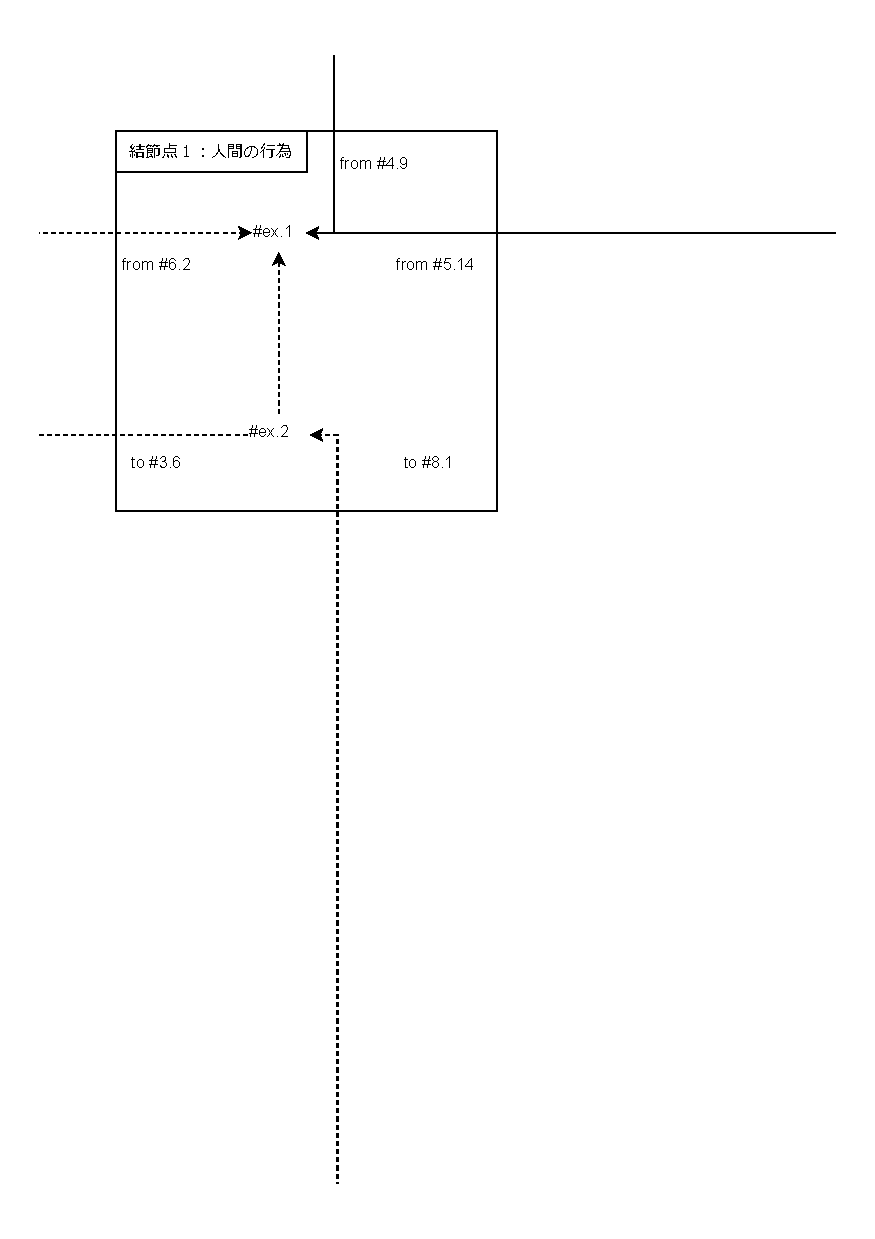
\includepdf[pages=-, scale=0.90, pagecommand={\thispagestyle{plain}}]{../figures/ex.pdf}

\section{神経症と精神病における葛藤の解消}\label{ux795eux7d4cux75c7ux3068ux7cbeux795eux75c5ux306bux304aux3051ux308bux845bux85e4ux306eux89e3ux6d88}

\subsection{心的構造の基本概念}\label{ux5fc3ux7684ux69cbux9020ux306eux57faux672cux6982ux5ff5}

自我とリアリティの体系(「心的構造」)は、各個人の幼児期にその大まかな形態が確定される。心的構造により、葛藤の解消の仕方には違いがある。心的構造は「神経症」と「精神病」に大別される。

\begin{note}{}
  \begin{itemize}
    \tightlist
    \item{\#6.1}自我とリアリティの体系(=「心的構造」)は、  各個人の幼児期にその大まかな形態が確定される。
    \item{\#6.2}心的構造により、  葛藤の解消の仕方には違いがある。
    \item{\#6.3}心的構造は「神経症」と「精神病」に大別される。
  \end{itemize}
\end{note}

\subsection{神経症における父性隠喩と防衛の方法}\label{ux795eux7d4cux75c7ux306bux304aux3051ux308bux7236ux6027ux96a0ux55a9ux3068ux9632ux885bux306eux65b9ux6cd5}

神経症者は、幼児期に対象\(a\)の顕現に対して防衛する機制としての「父性隠喩」を確立している(「分離」)。父性隠喩とは、「シニフィアンの体系の全体に対して固定的な意味を保証するシニフィアン(「象徴的ファルス」)を持つアクター(「現実的父」)が存在する」という形式の「幻想」を信じることで生じる、「シニフィアンの体系の全体に対して象徴的ファルスに影響を受けた意味が付与される仕組み」である。つまり、非一貫的なものである大他者が、現実的父により統御され、その任意の部分の意味は象徴的ファルスにより保証されるということである。父性隠喩を確立するとは、「父性の欺瞞を受け入れる」ことであり、「幻想を形成する」ことである(「分離」)。神経症者は、父性隠喩を用いて対象\(a\)を隠喩化(「抑圧」)することで、対象\(a\)の顕現に対して防衛する。

\begin{note}{}
  \begin{itemize}
    \tightlist
    \item{\#6.4}神経症者は、  幼児期に対象$a$の顕現に対して防衛する機制としての「父性隠喩」を確立している(=「分離」)。
    \item{\#6.5}父性隠喩とは、「シニフィアンの体系の全体に対して固定的な意味を保証するシニフィアン(=「象徴的ファルス」)を持つアクター(=「現実的父」)が存在する」(=非一貫的なものである大他者が、現実的父により統御され、その任意の部分の意味は象徴的ファルスにより保証される)という形式の「幻想」を信じることで生じる、「シニフィアンの体系の全体に対して象徴的ファルスに影響を受けた意味が付与される仕組み」である。
    \item{\#6.6}父性隠喩を確立するとは、「父性の欺瞞を受け入れる」ことであり、「幻想を形成する」ことである(=「分離」)。
    \item{\#6.7}神経症者は、父性隠喩を用いて対象$a$を隠喩化(=「抑圧」)することで、対象aの顕現に対して防衛する。
  \end{itemize}
\end{note}

\subsection{精神病者による防衛の方法}\label{ux7cbeux795eux75c5ux8005ux306bux3088ux308bux9632ux885bux306eux65b9ux6cd5}

精神病者は、幼児期に対象\(a\)の顕現に対して防衛しなければならない状況を経験しておらず、そのため父性隠喩を確立してもいない。精神病者は、対象\(a\)を意識から排除する(「否認」「知ろうとしない」)ことで、対象\(a\)の顕現に対して防衛する。

\begin{note}{}
  \begin{itemize}
    \tightlist
    \item{\#6.8}精神病者は、幼児期に対象$a$の顕現に対して防衛しなければならない状況を経験しておらず、そのため父性隠喩を確立してもいない。
    \item{\#6.9}精神病者は、対象$a$を意識から排除する
      \begin{itemize}
        \tightlist
        \item (=「否認」)
        \item (=「知ろうとしない」)
      \end{itemize}ことで、対象$a$の顕現に対して防衛する。
  \end{itemize}
\end{note}

\subsection{神経症と精神病における症状の違い}\label{ux795eux7d4cux75c7ux3068ux7cbeux795eux75c5ux306bux304aux3051ux308bux75c7ux72b6ux306eux9055ux3044}

修正の結果構築される自我とリアリティが、他の人間個体のそれからは整合性を保てない場合、そのような修正を行った人間個体は「病的」であるとされる。神経症者の「症状」は、反復強迫する対象\(a\)となった出来事(\(\textrm{S}_1\))を、「隠喩」的もしくは「文字」的あるいは「音素」的につながりのある「言葉」を経由する(\(\textrm{S}_1\rightarrow\textrm{S}_2\))ことで、間接的に解消して満足するものである(「象徴的加工」)。一方、精神病者の「症状」は、反復強迫する対象\(a\)となった出来事(\(\textrm{S}_1\))を、直接的・無媒介的に呼び起して解決することによって、解消して満足するものである。直接的・無媒介的に呼び起された出来事は、「パラノイア」の場合では、「妄想形成(\(\textrm{S}_1\rightarrow\textrm{S}_2\))」によって解決され、「スキゾフレニー」の場合では、シニフィアンの体系を用いずにそのまま身体で享楽を受け止める(「\(\textrm{S}_1\)の散乱状態」)。

\begin{note}{}
  \begin{itemize}
    \tightlist
    \item{\#6.10}修正の結果構築される自我とリアリティが、他の人間個体のそれからは整合性を保てない場合、そのような修正を行った人間個体は「病的」であるとされる。
    \item{\#6.11}神経症者の「症状」は、反復強迫する対象$a$となった出来事($\textrm{S}_1$)を、「隠喩」的もしくは「文字」的あるいは「音素」的につながりのある「言葉」を経由する($\textrm{S}_1\rightarrow\textrm{S}_2$)ことで、間接的に解消して満足するものである(=「象徴的加工」)。
    \item{\#6.12}精神病者の「症状」は、反復強迫する対象$a$となった出来事($\textrm{S}_1$)を、直接的・無媒介的に呼び起して解決することによって、解消して満足するものである。
    \item{\#6.13}直接的・無媒介的に呼び起された出来事は、「パラノイア」の場合では、「妄想形成($\textrm{S}_1\rightarrow\textrm{S}_2$)」によって解決される。
    \item{\#6.14}直接的・無媒介的に呼び起された出来事は、「スキゾフレニー」の場合では、シニフィアンの体系を用いずにそのまま身体で享楽を受け止める(=「$\textrm{S}_1$の散乱状態」)。
  \end{itemize}
\end{note}

\subsection{この章のまとめ}\label{ux3053ux306eux7ae0ux306eux307eux3068ux3081}

あ

\newpage
\includepdf[pages=-, scale=0.90, pagecommand={\thispagestyle{plain}}]{../figures/図6.pdf}

\section{エディプス・コンプレックスの諸段階}\label{ux30a8ux30c7ux30a3ux30d7ux30b9ux30b3ux30f3ux30d7ux30ecux30c3ux30afux30b9ux306eux8af8ux6bb5ux968e}

\subsection{幻想の形成過程}\label{ux5e7bux60f3ux306eux5f62ux6210ux904eux7a0b}

幻想の形成は、下記のように行われる。まず、幼児期において予期されない体験としての対象\(a\)が顕現した際に、養育者がそれを繰り返し解決するという前段階がある。その段階において、養育者は対象\(a\)の解消と結びつけて認識される。養育者は様々な感覚的特徴を持ち、また様々な働きかけを幼児に対して繰り返し行う。養育者の現前と養育者の様々な働きかけは、幼児の脳の中で対象\(a\)の解消(=満足)と結びついたシニフィアンとして蓄積されていく。そうして形成されるシニフィアンの体系が「大他者(=A)(=『(精神分析的)母』)」として前象徴界を形成する(=「前エディプス期」)。

\begin{note}{}
  \begin{itemize}
    \tightlist
    \item{\#7.1}
      幻想の形成は、下記のように行われる。
    \item{\#7.2}
      まず、幼児期において予期されない体験としての対象$a$が顕現した際に、養育者がそれを繰り返し解決するという前段階がある。
    \item{\#7.3}
      その段階において、養育者は対象$a$の解消と結びつけて認識される。
    \item{\#7.4}
      養育者は様々な感覚的特徴を持ち、また様々な働きかけを幼児に対して繰り返し行う。
    \item{\#7.5}
      養育者の現前と養育者の様々な働きかけは、幼児の脳の中で対象aの解消(=満足)と結びついたシニフィアンとして蓄積されていく。
    \item{\#7.6}
      そうして形成されるシニフィアンの体系が「大他者(=A)(=『(精神分析的)母』)」として前象徴界を形成する(=「前エディプス期」)。
  \end{itemize}
\end{note}

\subsection{エディプス第一の時}\label{ux30a8ux30c7ux30a3ux30d7ux30b9ux7b2cux4e00ux306eux6642}

しかし、大他者は以下の二点で対象\(a\)を十全に解消することはない: -
シニフィアンは体験との予測誤差をゼロにすることはない -
養育者は現前と不在を繰り返し、幼児を不安にさせる

上記二点が「大他者の非一貫性(=\(\cancel{\textrm{A}}\))」を形成する(=「不満」)。そこで、幼児は「大他者を一貫したものにする要素(=「ファルス」)」を探し求める。このとき、幼児に取ってファルスは「自分が『それ』になることができるかもしれないもの」としての「想像的ファルス」として現れている。

\begin{note}{}
  \begin{itemize}
    \tightlist
    \item{\#7.7}
      しかし、大他者は以下の二点で対象aを十全に解消することはない。
      \begin{itemize}
          \tightlist
          \item
          シニフィアンは体験との予測誤差をゼロにすることはない
          \item
          養育者は現前と不在を繰り返し、幼児を不安にさせる
        \end{itemize}
      上記二点が「大他者の非一貫性(=$\cancel{\textrm{A}}$)」を形成する(=「不満」)。
    \item{\#7.8}
      そこで、幼児は「大他者を一貫したものにする要素(=「ファルス」)」を探し求める。
    \item{\#7.9}
      このとき、幼児に取ってファルスは「自分が『それ』になることができるかもしれないもの」としての「想像的ファルス」として現れている。
  \end{itemize}
\end{note}

\subsection{エディプス第二の時における想像的父による剥奪}\label{ux30a8ux30c7ux30a3ux30d7ux30b9ux7b2cux4e8cux306eux6642ux306bux304aux3051ux308bux60f3ux50cfux7684ux7236ux306bux3088ux308bux5265ux596a}

エディプス第一の時において、養育者が「養育者の現前と不在を司る対象(=「(精神分析的)父」)」をシニフィアンとして幼児に示すとき、幼児は「父」を用いた幻想の構築を開始する。父が父として幼児に作用するためには、父は幼児の前に現前するものから超越していなければならないため、父は幼児の前に現前してはならない。この段階では、幼児は父を「大他者からファルスを『剥奪』した『想像的父』」として解釈するようになる。

\begin{note}{}
  \begin{itemize}
    \tightlist
    \item{\#7.10}
      エディプス第一の時において、養育者が「養育者の現前と不在を司る対象(=「(精神分析的)父」)」をシニフィアンとして幼児に示すとき、幼児は「父」を用いた幻想の構築を開始する。
    \item{\#7.11}
      父が父として幼児に作用するためには、父は幼児の前に現前するものから超越していなければならないため、父は幼児の前に現前してはならない。
    \item{\#7.12}
      まず、幼児は父を「大他者からファルスを『剥奪』した『想像的父』」として解釈するようになる。
  \end{itemize}
\end{note}

\subsection{エディプス第三の時における現実的父による去勢}\label{ux30a8ux30c7ux30a3ux30d7ux30b9ux7b2cux4e09ux306eux6642ux306bux304aux3051ux308bux73feux5b9fux7684ux7236ux306bux3088ux308bux53bbux52e2}

しかし、このとき父は「ファルスを持つ者」としても現れている。その側面を受容するとき、幼児はファルスの存在をファルスが現前しない状況のまま信じられるようになるので、幼児は大他者の非一貫性を大他者の本質として認められるようになる(=大他者の「去勢」を受け入れる)(=S(\(\cancel{\textrm{A}}\)))。幼児に大他者の去勢を認めさせる者としての父を「現実的父」と呼ぶ。

\begin{note}{}
  \begin{itemize}
    \tightlist
    \item{\#7.13}
      しかし、このとき父は「ファルスを持つ者」としても現れている。その側面を受容するとき、幼児はファルスの存在をファルスが現前しない状況のまま信じられるようになるので、幼児は大他者の非一貫性を大他者の本質として認められるようになる(=大他者の「去勢」を受け入れる)(=S($\cancel{\textrm{A}}$))。
    \item{\#7.14}
      幼児に大他者の去勢を認めさせる者としての父を「現実的父」と呼ぶ。
  \end{itemize}
\end{note}

\subsection{象徴的父・象徴的ファルス・欲望の主体}\label{ux8c61ux5fb4ux7684ux7236ux8c61ux5fb4ux7684ux30d5ux30a1ux30ebux30b9ux6b32ux671bux306eux4e3bux4f53}

父がファルスを持つと解釈されるとき、父は超越的な「法」によって大他者を統御する者と解釈されるようになる。このような父を「象徴的父(=『父の名』)」と呼ぶ。父が持つ法の根拠としてのファルスは「象徴的ファルス」と呼ばれる。これは、幼児が自身の対象\(a\)について「父および父の持つファルスを用いることで究極的には解決可能なものである」と解釈できるようになることと等価である。そこから、主体は対象\(a\)を解消するために自身もファルスを持つことを「欲望」するようになる(=「欲望の主体」の誕生)。

\begin{note}{}
  \begin{itemize}
    \tightlist
    \item{\#7.15}
      父がファルスを持つと解釈されるとき、父は超越的な「法」によって大他者を統御する者と解釈されるようになる。
    \item{\#7.16}
      このような父を「象徴的父(=『父の名』)」と呼ぶ。
    \item{\#7.17}
      父が持つ法の根拠としてのファルスは「象徴的ファルス」と呼ばれる。
    \item{\#7.18}
      これは、幼児が自身の対象aについて「父および父の持つファルスを用いることで究極的には解決可能なものである」と解釈できるようになることと等価である。
    \item{\#7.19}
      そこから、主体は対象aを解消するために自身もファルスを持つことを「欲望」するようになる(=「欲望の主体」の誕生)。
  \end{itemize}
\end{note}

\subsection{精神分析的な男と女}\label{ux7cbeux795eux5206ux6790ux7684ux306aux7537ux3068ux5973}

現実的父に同一化し、自身も象徴的ファルスを父のように持とうとする主体を「(精神分析的)男」という。

象徴的ファルスに同一化し、ファルスを持つ現実的父に欲望されることでファルスを間接的に持とうとする主体を「(精神分析的)女」という。

\begin{note}{}
  \begin{itemize}
    \tightlist
    \item{\#7.20}
      現実的父に同一化し、自身も象徴的ファルスを父のように持とうとする主体を「(精神分析的)男」という。
    \item{\#7.21}
      象徴的ファルスに同一化し、ファルスを持つ現実的父に欲望されることでファルスを間接的に持とうとする主体を「(精神分析的)女」という。
  \end{itemize}
\end{note}

\subsection{この章のまとめ}\label{ux3053ux306eux7ae0ux306eux307eux3068ux3081}

あ

\newpage
\includepdf[pages=-, scale=0.90, pagecommand={\thispagestyle{plain}}]{../figures/図7.pdf}

\section{神経症的主体における四つのディスクールと自然についての理解}\label{ux795eux7d4cux75c7ux7684ux4e3bux4f53ux306bux304aux3051ux308bux56dbux3064ux306eux30c7ux30a3ux30b9ux30afux30fcux30ebux3068ux81eaux7136ux306bux3064ux3044ux3066ux306eux7406ux89e3}

\subsection{ディスクールの要素}\label{ux30c7ux30a3ux30b9ux30afux30fcux30ebux306eux8981ux7d20}

神経症的な欲望の主体が対象\(a\)を「(〈父〉により解決される)問題」とするとき、主体はその問題に対して「(〈父〉という)根拠」と「(問題が解決された結果である)結論」が存在すると信じている(\#8.1)。このように解釈をするとき、神経症者の思考や行動を表現する四つの要素を用いて、この章で説明する「四つのディスクール」を描くことができる(\#8.2)。この四つの要素は、

\[a \rightarrow \cancel{\textrm{S}} \rightarrow \textrm{S}_1 \rightarrow \textrm{S}_2 \rightarrow a \rightarrow ...\]

という順に並べられる。つまり、「予測誤差が思考としての主体を作動させ、新しいシニフィアンの秩序を形成するが、そうして形成された秩序からも予測誤差が必ず発生する」という思考の\mbox{弁証法}\index{べんしょうほう@弁証法}がここにもみられるのだ。

\begin{note}{}
  \begin{itemize}
    \tightlist
    \item{\#8.1}
      神経症的な欲望の主体が対象aを「(〈父〉により解決される)問題」とするとき、主体はその問題に対して「(〈父〉という)根拠」と「(問題が解決された結果である)結論」が存在すると信じている。
    \item{\#8.2}
      このように解釈をするとき、
      \begin{itemize}
          \tightlist
          \item{$a$}
          対象あるいは残余$a$。転じて、予測誤差としての不確実性、加えて、そこにファルスが与えられるべきとされるもの
          \item{$\cancel{\textrm{S}}$}
          欲望の主体。対象$a$の解消を試みてシニフィアンを操作する
          \item{$\textrm{S}_1$}
          象徴的父。転じて、シニフィアンを連鎖させて構築する「言説」の根拠であり、根拠の選択の仕方により規定される「問いの枠組み(プロブレマティク)」
          \item{$\textrm{S}_2$}
          象徴的父がもたらす法。転じて、言説の結論であり、問いの枠組みにおいて根拠に従属する諸命題
        \end{itemize}
    の四つの要素を用いて、神経症者の思考や行動を表現する「四つのディスクール」を描くことができる。
  \end{itemize}
\end{note}

ここで付言しておくべきことは、「問いの枠組み(プロブレマティク)」は問いだけでなく、答えをも方向づけてしまうということだ(註1)。なぜならば、答えというものは常に「問いに対する答え」だからである。このことを理解するために、西洋近代哲学における「経験論(外界についての経験を積み上げることで、世界の真理に辿り着けるとする考え方)」と「合理論(疑うことができない思考の原理原則を分析することで、世界の真理に辿り着けるとする)」という伝統的な二つの潮流を取り上げる。この両者の違いは、経験論が真理を客体の側に、合理論が真理を主体の側に位置づけている点にある。しかし、それは逆に言えば、どちらの考え方も主体/客体/真理という共通した語彙(および、そこに付随する関係性)を持っているということでもある。経験論と合理論という対立は、共通した一つの「問いの枠組み」から生じた二つの答えにすぎないのだ。経験論と合理論の例についていえば、それらは確かに様々な説明を生み出す基盤となる\(\textrm{S}_1\)ではあるのだが、それらが派生的な知\(\textrm{S}_2\)としての位置におかれるような、より根源的な枠組み\(\textrm{S}_1\)としての「主体/客体/真理」という語彙が存在しているわけだ(こうした、ある世界観が持つ階層性については第三章第二節で詳しく扱う)。

そして、このプロブレマティクが西洋近代のものであるように、「問いの枠組み」は歴史的なシニフィアンの体系の変遷に伴って形成されるものだ。実際、近代以前のスコラ学では普遍的なものをめぐる「実念論」と「唯名論」の対立が普遍論争という論争を引き起こしていたし、西洋以外では西洋近代ともスコラ学とも異なる問いの枠組みがそれに起因する学問的探求を支えていた。「問いの枠組み(=\(\textrm{S}_1\))」は、その時代、その場所、その集団ごとに採用される「世界を秩序立てて説明する座標軸の取り方」であり、その座標軸の取り方によって、世界の様々なもの(=\(\textrm{S}_2\))の説明のされ方も定まり、その限界(=\(a\))も自ずと定まるのだ。

\begin{itemize}
\tightlist
\item
  (註1) 今村(2007:355-357)\cite{Imamura1}参照。
\end{itemize}

\subsection{ディスクールの構造}\label{ux30c7ux30a3ux30b9ux30afux30fcux30ebux306eux69cbux9020}

四つのディスクールを構成する各位置には、それぞれの役割がある(\#8.3)。この四つの位置は、思考の\mbox{弁証法}\index{べんしょうほう@弁証法}において「動因が他者を新たな位置に据える際に、そのような仕方で動因が動かなければならない原因が真理にあり、動因が他者を新たな位置に据えた結果として生産物が発生してしまうという」ということを意味している。

\begin{note}{}
  \begin{itemize}
    \tightlist
    \item{\#8.3}
      四つのディスクールを構成する各位置には、下記のような役割がある。
      \begin{itemize}
          \tightlist
          \item
          主体が当初同一化しているものが真理である。
          \item
          真理には十全でないところがあり、それが動因を発生させる。
          \item
          動因は他者に働きかけ、他者は生産物を算出する。
          \item
          生産物は真理を十全にすべく生じたものだが、それは実現しない。
        \end{itemize}

$$
\uparrow\frac{\mathrm{動因}}{\mathrm{真理}}\genfrac{}{}{0pt}{}{\longrightarrow}{//}\frac{\mathrm{他者}}{生産物}\downarrow
$$
  \end{itemize}
\end{note}

ここからはエディプス・コンプレックスの流れに即して四つのディスクールをみていくが、この四つのディスクールは、主体が世界を理解するプロセスに対応しているとも言える。そこで、本章では具体例として人間が自然を理解する場合ではどのように四つのディスクールが働いているのかも見ていくことにする。

\subsection{分析家のディスクール}\label{ux5206ux6790ux5bb6ux306eux30c7ux30a3ux30b9ux30afux30fcux30eb}

分離が始まる瞬間(=エディプス第二の時)に対応するのが、右の「\mbox{分析家のディスクール}\index{ぶんせきかのでぃすくーる@分析家のディスクール}」である(\#8.4)。このようなディスクールの具体例としては、新しい世界観の提唱を挙げることができるだろう。天体運動論は、その中でも特にスッキリとした数学的解決が得られた例として参照することができる。そこでは、まず所与の感覚としての夜闇と光点の動き
\(\textrm{S}_2\) がある。その乱雑な所与の感覚は不安 \(a\)
を催し、それを理解しようとする主体 \(\cancel{\textrm{S}}\)
を作動させる。そうして、地球の周りを天体が回るという「天動説」のアイデアが\(\textrm{S}_1\)として設定される。この設定によって、天空を巡る光点の群れという混沌を秩序付けられるようになる。

\begin{note}{}
  \begin{itemize}
    \tightlist
    \item{\#8.4}
      分離が始まる瞬間(=エディプス第二の時)に対応するのが、「\mbox{分析家のディスクール}\index{ぶんせきかのでぃすくーる@分析家のディスクール}」である。
      \begin{itemize}
          \tightlist
          \item
          主体は既存のシニフィアンの体系(=$\textrm{S}_2$)に同一化している。
          \item
          シニフィアンの体系には非一貫性があり、予測誤差としての残余$a$が生じる。
          \item
          残余$a$は主体(=$\cancel{\textrm{S}}$)を作動させ、主体は革新的な視点(=$\textrm{S}_1$)を得る
          \item
          新たな視点は既存のシニフィアンの体系と調和せず(=$\textrm{S}_2//\textrm{S}_1$)、シニフィアンの体系を組みかえはじめる
        \end{itemize}このディスクールは不安定であり、速やかに下記の「\mbox{主人のディスクール}\index{しゅじんのでぃすくーる@主人のディスクール}」へと移行する。

$$
\uparrow\frac{a}{\mathrm{S_2}}\genfrac{}{}{0pt}{}{\longrightarrow}{//}\frac{\cancel{\textrm{S}}}{\mathrm{S_1}}\downarrow
$$
  \end{itemize}
\end{note}

\subsection{主人のディスクール}\label{ux4e3bux4ebaux306eux30c7ux30a3ux30b9ux30afux30fcux30eb}

父性隠喩を確立する段階(=「エディプス第三の時」)に対応するのが、\mbox{主人のディスクール}\index{しゅじんのでぃすくーる@主人のディスクール}である(\#8.5)。天体運動論の例でいえば、天動説というアイデアに基づいて所与の感覚を天体の動きとして秩序付ける動きが始まることで、主体が抱える不安は解消に向かうことになる(=\(\uparrow\frac{\textrm{S}_1}{\cancel{\textrm{S}}}\))。そうして、そのアイデアに沿って、個々の天体がどれくらいの周期で天球上を巡るかという具体的な説明がされるようになる(=\(\textrm{S}_1\rightarrow\textrm{S}_2\))。だが、天体の軌道は地球を中心とした単純な円によってはうまく説明しきれない。惑星は天球上を逆行することもあるからだ。こうして、理論との誤差(=\(a\))が生まれる(=\(\frac{\textrm{S}_2}{a}\downarrow\))。この誤差は、素朴な天動説によっては解消することができない(\(\cancel{\textrm{S}}//a\))。

\begin{note}{}
  \begin{itemize}
    \tightlist
    \item{\#8.5}
      父性隠喩を確立する段階(=「エディプス第三の時」)に対応するのが、\mbox{主人のディスクール}\index{しゅじんのでぃすくーる@主人のディスクール}である。
      \begin{itemize}
          \tightlist
          \item
          主体(=$\cancel{\textrm{S}}$)は新たな根拠となるシニフィアン(=$\textrm{S}_1$)に依拠する。
          \item
          新たな根拠に基づいて様々な命題が生み出されていく(=$\textrm{S}_1\rightarrow\textrm{S}_2$)。
          \item
          しかし、そうして構築された新たなシニフィアンの体系にも非一貫性(=$a$)がある。
          \item
          この非一貫性は、このディスクールで最初に欲望の主体が解消しようとしたものとは異なる新たな残余$a$である。
          \item
          生み出された残余$a$と主体との間には断絶があるが(=$\cancel{\textrm{S}}//a$)、主体はこの断絶が克服されうるものなのだという幻想を信じている(=$\cancel{\textrm{S}}$◇a)。
        \end{itemize}

$$
\uparrow\frac{\mathrm{S_1}}{\cancel{\textrm{S}}}\genfrac{}{}{0pt}{}{\longrightarrow}{//}\frac{\mathrm{S_2}}{a}\downarrow
$$
  \end{itemize}
\end{note}

惑星の動きほどスッキリとした解決が得られる場合は少ないが、自然の動きについても本章でみるのと同じプロセスを経て理解が進むことになる。まずは混沌とした所与の中に、秩序の源泉となる点が打ち立てられる(=\mbox{分析家のディスクール}\index{ぶんせきかのでぃすくーる@分析家のディスクール})。そして、そこを根拠として物事が体系的に説明されるようになり、それに合わせて人は制度や仕組みを作るようになるのだ(=\mbox{主人のディスクール}\index{しゅじんのでぃすくーる@主人のディスクール})。

なお、ある対象の範囲について物事を説明するアイデア(=\(\textrm{S}_1\))が打ち立てられるとき、そのアイデアはより根源的に社会を支える別のアイデア(=\(\textrm{S}_1\))との整合性も問われることになる(繰り返しになるが、こうした世界観の階層性については第三章第二節で詳しく扱う)。近代以前の西洋において、天動説というアイデア(=\(\textrm{S}_1\))は、より社会を根源的に支えていたキリスト教的世界観(=\(\textrm{S}_1\))とも整合的なものだった。たとえば、地球を宇宙の中心に据える世界解釈は、「神の天地創造により生まれた特別な存在としての地」という地球についての解釈と整合的であった。また、旧約聖書内の記述(『ヨシュア記』10章13節など)も地球が不動の天体である根拠とされた(註1)。

\begin{itemize}
\tightlist
\item
  (註1) 船越(1885)\cite{Funakoshi}参照。
\end{itemize}

\subsection{大学のディスクール}\label{ux5927ux5b66ux306eux30c7ux30a3ux30b9ux30afux30fcux30eb}

確立した父性隠喩について、現実的父に同一化し象徴的ファルスを持っていると思いたい者は「\mbox{大学のディスクール}\index{だいがくのでぃすくーる@大学のディスクール}」を好むようになる(\#8.6)。\mbox{大学のディスクール}\index{だいがくのでぃすくーる@大学のディスクール}は、\mbox{分析家のディスクール}\index{ぶんせきかのでぃすくーる@分析家のディスクール}や\mbox{主人のディスクール}\index{しゅじんのでぃすくーる@主人のディスクール}とは異なり、新たな枠組みの創始を望まない官僚主義的なディスクールだ(註1)。例えば、天動説という世界観(=\(\textrm{S}_1\))に基づいた説明(=\(\uparrow\frac{\textrm{S}_2}{\textrm{S}_1}\))では、説明できないままに留まっていた惑星の軌道(=\(a\))に対して、歴史上いくつかの概念が追加された。そうすることによって、理論は精緻化され、予測誤差を縮小することができたからだ(註2)。実際、それらの概念を追加することによって惑星の逆行もかなり精度よく計算できるようになる。だが、予測誤差がゼロになることはなく、したがって認識を発展させる\mbox{弁証法}\index{べんしょうほう@弁証法}的作用としての主体(=\(\cancel{\textrm{S}}\))も燻り続ける(=\(\frac{a}{\cancel{\textrm{S}}}\downarrow\))。とはいえ、追加された概念によって天体の軌道予測は精緻にし続けていくことができるのだから、\mbox{大学のディスクール}\index{だいがくのでぃすくーる@大学のディスクール}に立つ主体は、あえて天動説を放棄して混沌を再び解き放とうとは思わないだろう(=\(\textrm{S}_1//\cancel{\textrm{S}}\))。

\begin{note}{}
  \begin{itemize}
    \tightlist
    \item{\#8.6}
      確立した父性隠喩について、現実的父に同一化し象徴的ファルスを持っていると思いたい者は「\mbox{大学のディスクール}\index{だいがくのでぃすくーる@大学のディスクール}」を好むようになる。
      \begin{itemize}
          \tightlist
          \item
          主体(=$\cancel{\textrm{S}}$)は言説の根拠(=$\textrm{S}_1$)を所持する者に同一化している。
          \item
          言説の根拠はそれ単独ではシニフィアンの体系を形成できず、自身に基づいた様々な命題を持っている(=$\uparrow\frac{\textrm{S}_2}{\textrm{S}_1}$)。
          \item
          様々な命題は、新たな残余$a$を既存の問いの枠組みを保持したまま解決しようとする(=$\textrm{S}_2\rightarrow a$)。
          \item
          だが、その試みは不徹底に終わり、新たな欲望の主体(=$\cancel{\textrm{S}}$)を発生させる。
          \item
          しかし、新たな欲望の主体に従って再びシニフィアンの体系を組みかえることは、現在の主体の同一化を放棄させることを意味するので、この新たな欲望の主体は抑圧される。
        \end{itemize}

$$
\uparrow\frac{\mathrm{S_2}}{\mathrm{S_1}}\genfrac{}{}{0pt}{}{\longrightarrow}{//}\frac{a}{\cancel{\textrm{S}}}\downarrow
$$
  \end{itemize}
\end{note}

\begin{itemize}
\tightlist
\item
  (註1) 向井(2016: 381)\cite{Mukai}を参照。
\item
  (註2)
  精緻化された天動説ではは「離心円(地球の中心とは違う点に中心を持つ円)」と「従円(周転円に比べて大きな円。この従円が離心円になっている)・周転円(従円の円周上に中心を持つ点)・エカント(地球の中心とも従円の中心とも違う場所に、エカント点を打ち、周転円の中心をエカントから見て一定の角速度で動くようにする)」の概念が必要となる。詳しい説明はホイル(1973=1974)\cite{Hoyle}を参照。今日の私たちは、惑星は太陽を焦点とする楕円軌道を回るということ、その際に惑星は面積速度が一定になるように運動することなどを知っている。そのことを知っているからこそ、そこから計算して天体の軌道を計算することなど簡単だと思い込んでいる。だが、地上から見える光点の不可解な動きのみを出発点としてこの科学的知見に至ることは大変難しい。
\end{itemize}

\subsection{ヒステリー者のディスクール}\label{ux30d2ux30b9ux30c6ux30eaux30fcux8005ux306eux30c7ux30a3ux30b9ux30afux30fcux30eb}

確立した父性隠喩について、象徴的ファルスに同一化し現実的父に欲望されることを欲望する者は、「\mbox{ヒステリー者のディスクール}\index{ひすてりーしゃのでぃすくーる@ヒステリー者のディスクール}」を好むようになる(\#8.7)。\(\textrm{S}_1\)は超越的な対象についてのシニフィアンであるが、それ自体が超越的であるわけではないため、その権威を失墜させることができるという点がポイントだ。

\begin{note}{}
  \begin{itemize}
    \tightlist
    \item{\#8.7}
      確立した父性隠喩について、象徴的ファルスに同一化し現実的父に欲望されることを欲望する者は右の「\mbox{ヒステリー者のディスクール}\index{ひすてりーしゃのでぃすくーる@ヒステリー者のディスクール}」を好むようになる。
      \begin{itemize}
          \tightlist
          \item
          主体は、対象$a$の位置に来るべき象徴的ファルスに同一化するために、ファルスに仮装する(=$\uparrow\frac{\cancel{\textrm{S}}}{a}$)。
          \item
          仮装した主体は自身では対象$a$を解消できない。
          \item
          仮装した主体は対象$a$を解消すべく、現実的父になりえそうな他者に働きかけて(=$\cancel{\textrm{S}}\rightarrow\textrm{S}_1$)様々な命題を吐き出させる(=$\frac{\textrm{S}_1}{\textrm{S}_2}\downarrow$)。
          \item
          しかし、いかなる命題も対象$a$そのものを根絶することはない(=$a//\textrm{S}_2$)。
          \item
          そのため、それらの命題の根拠(=$\textrm{S}_1$)も失墜する。
        \end{itemize}

$$
\uparrow\frac{\cancel{\textrm{S}}}{a}\genfrac{}{}{0pt}{}{\longrightarrow}{//}\frac{\mathrm{S_1}}{\mathrm{S_2}}\downarrow
$$
  \end{itemize}
\end{note}

このような\mbox{ヒステリー者のディスクール}\index{ひすてりーしゃのでぃすくーる@ヒステリー者のディスクール}は、世界を理解するプロセスにおいては「予測誤差を常に前面に掲げ続け、既存の世界観の限界を明らかにし、その正当性や信頼を失墜させる」という革新的な動きをもたらす。そこでは、まず予測誤差あるいは不確実性(=\(a\))の解決(=\(\uparrow\frac{\cancel{\textrm{S}}}{a}\))を、既に確立された視点/問題の枠組み/権威(=\(\textrm{S}_1\))によって達成しようとする。だが、\(\textrm{S}_1\)は有限の知(=\(\textrm{S}_2\))しか生みだせず(=\(\frac{\textrm{S}_1}{\textrm{S}_2}\downarrow\))、それが予測誤差や不確実性を解決することはない(=\(a//\textrm{S}_2\))。こうして、\mbox{ヒステリー者のディスクール}\index{ひすてりーしゃのでぃすくーる@ヒステリー者のディスクール}は既存の世界観を頼ることで、かえって逆にその無能力を露呈させてしまう。その結果は\(\textrm{S}_1\)に対する失望に終わり、\(\textrm{S}_1\)は手段としての信頼を失墜させる。この\(\textrm{S}_1\)の失墜の結果、ヒステリー者は混乱の中に投げ出されてしまう。

周転円をいくら追加しても予測誤差がゼロにできない中でも、背後ではブラーエ(1546-1601)らによってそれまでよりも精密な計測データ
\(\textrm{S}_2\)
が溜まっていっていた。これらの計測データもまた、既存の世界観の中で用いられていた既存の計測機器を使用して貯められてきたきたものだ(=\(\frac{\textrm{S}_1}{\textrm{S}_2}\downarrow\))。こうして貯められたデータが、新しい天体モデルの誕生を準備することになった。

\subsection{分析家のディスクール、再び}\label{ux5206ux6790ux5bb6ux306eux30c7ux30a3ux30b9ux30afux30fcux30ebux518dux3073}

このような蓄積された知と混乱の中で、\mbox{分析家のディスクール}\index{ぶんせきかのでぃすくーる@分析家のディスクール}を通じて、人は新しい問題の枠組みを生み出す。天動説の例でいえば、天動説を唱えていたプトレマイオス(83頃-163頃)の著作についての批判的研究からコペルニクス(1473-1543)が太陽中心説(=地動説)を唱えた。しかし、この時点の地動説ではエカントが除去されたのみで、周転円の数が減ったわけでもなく、精度面でもそれまでの天動説より優位に立てたわけではなかった。つまり、コペルニクスの時点では地動説は完成していなかったのだ。地動説の完成は、ブラーエのデータをもとに天体の軌道を計算し、その軌道上で面積速度一定の法則などを発見したケプラー(1571-1630)の登場や、慣性の法則や金星の満ち欠けを発見したガリレイ(1564-1642)の登場、そして微積分法・古典力学・万有引力の法則を発見したニュートン(1642-1727)らの登場を待たねばならない。ニュートン力学というより根源的な枠組み\(\textrm{S}_1\)の成立によって、物体の運動が万有引力と運動方程式によって基礎付けられることとなり、そこから楕円軌道が説明されて、地動説が遂にその優位を確立するからである。

ただし、それらの発見によって地動説が完成し、天体の運動がより簡潔に説明できるようになったとしても、それは天動説が「論破」されたということを意味するわけではない。世界に起こる現象を説明するやり方は一通りではないからだ。例えば、「すべての物事は完全に自分中心で動いているのであって、そうでなうように思う他人はすべて錯覚に陥っているのだ。単純なモデルでは表せないことかもしれないが、実はそうなのだ」と矛盾なく言い張ることはできる。ただ、そうした不必要に複雑なモデルは、有用さの観点で劣っているため、世界を説明する手段として採用する者がいなくなりがちだというだけだ。こうして、人々が採用する世界観において、支持者の喪失と獲得を通じた「パラダイム転換(註1)」が起こることになる。

\begin{itemize}
\tightlist
\item
  (註1) クーン(1970=1971)\cite{Khun}を参照。
\end{itemize}

\subsection{この章のまとめ}\label{ux3053ux306eux7ae0ux306eux307eux3068ux3081}

本章では、神経症的主体における四つのディスクールについて、自然科学(特に天体運動論)を例に取りながら説明した。四つのディスクールは、主体が世界を理解していく過程で以下のように循環的に現れる:

\begin{enumerate}
\def\labelenumi{\arabic{enumi}.}
\tightlist
\item
  \mbox{分析家のディスクール}\index{ぶんせきかのでぃすくーる@分析家のディスクール}:

  \begin{itemize}
  \tightlist
  \item
    既存の理解(\(\textrm{S}_2\))に起因して予測誤差(\(a\))が生じることで、主体(\(\cancel{\textrm{S}}\))が作動し、新たな視点(\(\textrm{S}_1\))を見出す段階
  \item
    例:天体の動きという混沌から天動説という新しい世界観の誕生
  \end{itemize}
\item
  \mbox{主人のディスクール}\index{しゅじんのでぃすくーる@主人のディスクール}:

  \begin{itemize}
  \tightlist
  \item
    新たな視点(\(\textrm{S}_1\))に基づいて体系的な説明(\(\textrm{S}_2\))を構築する段階
  \item
    しかし、新たな予測誤差(\(a\))も生まれる
  \item
    例:天動説に基づく天体運動の体系的説明の確立
  \end{itemize}
\item
  \mbox{大学のディスクール}\index{だいがくのでぃすくーる@大学のディスクール}:

  \begin{itemize}
  \tightlist
  \item
    既存の枠組み(\(\textrm{S}_1\))を維持したまま、その中で説明(\(\textrm{S}_2\))を精緻化していく段階
  \item
    予測誤差(\(a\))は完全には解消されないが、枠組みは保持される
  \item
    例:周転円などの概念追加による天動説の精緻化
  \end{itemize}
\item
  \mbox{ヒステリー者のディスクール}\index{ひすてりーしゃのでぃすくーる@ヒステリー者のディスクール}:

  \begin{itemize}
  \tightlist
  \item
    予測誤差(\(a\))を前面に掲げ、既存の権威(\(\textrm{S}_1\))の限界を明らかにする段階
  \item
    既存の説明体系(\(\textrm{S}_2\))の不十分さが露呈する
  \item
    例:精密な観測データの蓄積による天動説の限界の顕在化
  \end{itemize}
\end{enumerate}

この循環を経て、再び\mbox{分析家のディスクール}\index{ぶんせきかのでぃすくーる@分析家のディスクール}が現れ、新たなパラダイムが生まれる(例:地動説の確立)。ただし、これは旧来の説明の「論破」を意味するわけではなく、より簡潔で有用な説明の採用という形でパラダイム転換が起こるのである。

\newpage
\includepdf[pages=-, scale=0.90, pagecommand={\thispagestyle{plain}}]{../figures/図8.pdf}

\chapter{四つのディスクールが形成する人間社会のダイナミズム}

\section{自然への抵抗としてのエンジニアリングと芸術}\label{ux81eaux7136ux3078ux306eux62b5ux6297ux3068ux3057ux3066ux306eux30a8ux30f3ux30b8ux30cbux30a2ux30eaux30f3ux30b0ux3068ux82b8ux8853}

\subsection{横溢する自然への抵抗としてのエンジニアリング}\label{ux6a2aux6ea2ux3059ux308bux81eaux7136ux3078ux306eux62b5ux6297ux3068ux3057ux3066ux306eux30a8ux30f3ux30b8ux30cbux30a2ux30eaux30f3ux30b0}

自由エネルギーの最小化としての葛藤の解消の帰結として、人間は自然を予測可能なものとするために、自然についての理解を体系化した上で、その知識に基づいて自然を制御する制度や仕組みを構築する。このような行為を第一部では「エンジニアリング」と呼ぼう(\#9.1)。このとき、エンジニアリングが持つダイナミズムを四つのディスクールを用いて表現することができる(\#9.2)。そのダイナミズムは、エンジニアリングによる捕獲を逃れる不確実性としての対象\(a\)により駆動される(\#9.3)。

\begin{note}{}
  \begin{itemize}
    \tightlist
    \item{\#9.1}自由エネルギーの最小化としての葛藤の解消の帰結として、人間は自然を予測可能なものとするために、
      \begin{itemize}
        \tightlist
        \item 自然についての知識を体系化し、
        \item その知識に基づいて自然を制御する制度や仕組みを構築する
      \end{itemize}(=「エンジニアリング」)。
    \item{\#9.2}エンジニアリングが持つダイナミズムは、四つのディスクールを用いて表現することができる。
    \item{\#9.3}このダイナミズムは、エンジニアリングによる捕獲を逃れる不確実性としての対象$a$により駆動される。
  \end{itemize}
\end{note}

この章では、四つのディスクールに沿ってエンジニアリングが持つダイナミズムを説明していく。だがその前に、第一部が述べるエンジニアリングと労働との関係について軽く触れておくことにしよう。それは、エンジニアリングや労働という言葉について、第十章や第十一章で扱うような、その二次的なあり方のイメージが広く染みつきすぎているからだ。この章で扱うエンジニアリングや労働をそうしたイメージに沿って理解してはならないということを、最初に説明しておきたいのである。

\subsection{労働のオリジナル(=本源的)なあり方としてのエンジニアリングとカイゼン、そしてアジャイルな組織}\label{ux52b4ux50cdux306eux30aaux30eaux30b8ux30caux30ebux672cux6e90ux7684ux306aux3042ux308aux65b9ux3068ux3057ux3066ux306eux30a8ux30f3ux30b8ux30cbux30a2ux30eaux30f3ux30b0ux3068ux30abux30a4ux30bcux30f3ux305dux3057ux3066ux30a2ux30b8ux30e3ux30a4ux30ebux306aux7d44ux7e54}

まず、生命が世界を生きる過程において、およそ何の予想外の出来事にも出会わないような時間は存在しないという事実について改めて確認するところから始めよう。この事実は、具体的なシニフィアンがあれば必ずその傍らに取りこぼされた純粋差異としての〈物〉があるがゆえに、その顕現が予想外の出来事となるという事情に起因する(\#9.4)。そこでは、私たちの無知の証である自然の横溢が、克服し征服すべきスリリングな知的興味の対象として表れている。

\begin{note}{}
  \begin{itemize}
    \tightlist
    \item{\#9.4}自然界において未来を厳密に予測しきることは不可能である。
  \end{itemize}
\end{note}

この事実は、エンジニアリングがどれほど発達しようとも、不確実性としての対象\(a\)が根絶されることはないということを意味している(\#9.5)。自然の横溢を前にして、エンジニアリングを行う人間は自身の認識を弁証法的に更新し、その成果を制度や仕組みに反映させ続けることになる。この意味で、生に満ちている予想外の出来事のすべてが、エンジニアリングの入り口になっている。

\begin{note}{}
  \begin{itemize}
    \tightlist
    \item{\#9.5}エンジニアリングがどれほど発達しようとも、不確実性としての対象$a$が根絶されることはない。
  \end{itemize}
\end{note}

この「生命にとって、予想外の出来事に出会わないような時間は存在しない」という命題は、生活の糧を得るための行動としての「労働」の場でも成り立つ。労働とは、まず第一に欲望の対象を生産する行為だといえる(ここでいう「生産」には、対象を市場の中に晒すことなどの社会的な行動も含まれる)。この欲望の対象は無から勝手に生じるのではなく、認識されるまでは謎でしかない自然の中から現れてくる。初めのうちは、欲望の対象は偶発的な事象に依存して発生するに留まることもありうる(例えば、「火の発生を落雷に頼る」や「獲物の兎が勝手に切り株に衝突して死ぬ」や「自分の所持品を高価な物と交換してくれる人に遭遇する」など)。この段階では、予測誤差は自然の恵みとしての偶発性自体と共にある。だが、そこから欲望の対象を人間が計画的に自然から取り出させるようになれば、その段階で自然から欲望の対象を取り出す生産方法についての認識が確立できたと言える(「火起こしの手法を確立する」や「獲物を捕まえる罠の作成法を確立する」や「所持品を交換したい人が集まる場を作る」など)。この段階では、予想外の出来事は認識に伴う取りこぼされた純粋差異としてその場に付随する(「たまたま、火起こしに使う棒が予想よりも少し湿っている」や「たまたま、その日は兎が通りがからなかった」や「たまたま、自分の所持品を欲望する人が現れなかった」など)。いずれにせよ、労働は予想外の出来事と共にあることになる。

そして、労働の場に予想外の出来事があるということは、労働を支える認識と行為にもそれが揺るがされる余地があるということだから、その克服は労働の「カイゼン」に繋がる。ここでいうカイゼンとは、私たちの認識と外界との間で発生する予測誤差の縮小に根本的な起源を持つものだ。その帰結は、単純な生産量の増加とは限らない。労働に伴う苦痛の削減や、生産する対象の変更、労働の目的の更新など、様々な帰結がありうる(例えば、「火おこしに使う棒を徹底的に乾かす方法を確立」できれば「火起こしの際の労力が減る」だろうし、「兎の生態に詳しくなる」ことができれば「罠の効率的な設置ができる」だろうし、「自分の所持品を欲する人を探り当てる方法が確立」できれば「所持品を交換しそびれるリスクが減る」あろう)。だが、そのどの場合でも、労働を支える認識は外界の実情により近づこうとすることになる(もちろん、認識はその際に変分ベイズ推論的に変わるので、一時的に外界の実情から遠のくこともありうる)。

カイゼンにおいて、認識とその産物は過去のそれらに強固に拘束されることはない。過去に作られた認識・制度・仕組みなどは必要とあれば撤廃されることになる。このような労働のあり方は、人間が原初の頃より自然と格闘しながら繰り広げてきた労働のオリジナル(=本源的)なあり方だといえるだろう。

このように、エンジニアリングの観点からみれば、労働は驚きの連続と共にある知的創造だと言える。このような「いきいき」とした労働は、社会の中で実現可能であり、それは多くの場所で実践されている(註1)。その典型が、「アジャイル」が全体に浸透しているような組織だ。アジャイルとは、不確実性と直面する機会を積極的に織り込むことでエンジニアリングのダイナミズムを活性化させて、より良い満足を生みだしていうとする思想のことだ(\#9.6)(註2)。そこでは、組織のあらゆる場所での発見が、組織の他の部分へと対話を通じて伝播していく。アジャイルな組織においては、階層的な秩序は存在しうるが、決して硬直的にはなっていない。予想外の出来事としての現実に向き合い、その不確実性を弁証法的に克服しようとる不断の運動が、アジャイルな組織を「いきいき」とした活動的なものにしている。

\begin{note}{}
  \begin{itemize}
    \tightlist
    \item{\#9.6}不確実性と直面する機会を積極的に織り込むことでエンジニアリングのダイナミズムを活性化させて、より良い満足を生みだしていこうとする思想を「アジャイル」という。
  \end{itemize}
\end{note}

そこには、労働についての批判的な議論で出てくるような「有無を言わさず従うしかない強制的な労働力の搾取」としての労働の面影はほとんどない(註3)。そうした労働は、エンジニアリングの産物が「疎外」を生むことによって生じた、労働の二次的な形態でしかないからだ。エンジニアリングの産物は認識を外化したものとしての仕組みや所持品に他ならないが、そうした認識を外化したものは自己自身ではない。そのため、それらは身体に対して予測誤差を生む結果へと必然的に帰結してしまう(註4)。このとき、その予測誤差を解決するために外化したものをカイゼンするのでなければ、その外化したものはやがて人間を疎外するようになるのだ。

そうした疎外が四つのディスクールをどのようなものに変えるかについては、次章で見ていくことになる。そこでは、四つのディスクールが、構造はそのままに、より抑圧的、あるいは搾取的な性格を持つようになる。だが、この章ではエンジニアリングと四つのディスクールとの関係に焦点を当てることにしよう。

\begin{itemize}
\tightlist
\item
  (註1)
  ここでの「いきいき」という副詞は、小田中によるものを用いた。その意味については小田中(2023)\cite{Odanaka}を参照。
\item
  (註2) 市谷/新井/小田中(2020)\cite{IchitaniEtAl}を参照。
\item
  (註3)
  今村(2024)\cite{Imamura2}には、労働がそのようなものとして捉えられてきた様子が記されている。
\item
  (註4) ==ヘーゲル『精神現象学』==
\end{itemize}

\subsection{エンジニアリングにおける主人のディスクール}\label{ux30a8ux30f3ux30b8ux30cbux30a2ux30eaux30f3ux30b0ux306bux304aux3051ux308bux4e3bux4ebaux306eux30c7ux30a3ux30b9ux30afux30fcux30eb}

エンジニアリングにおける主人のディスクール(\#9.7)とは、新しい思想(=\(\textrm{S}_1\))に基づいて法律/制度/仕組み(=\(\textrm{S}_2\))が策定される段階である。これらの策定により、社会は未規定なものから規定されたものとなる。しかし、それらの策定によってすべてが規定されつくすことはなく、必ず未規定な部分が残る(=\(\frac{\textrm{S}_2}{a}\downarrow\))。

\begin{note}{}
  \begin{itemize}
    \tightlist
    \item{\#9.7}エンジニアリングにおける主人のディスクールとは、
      \begin{itemize}
        \tightlist
        \item 新しく確立された視点や問題の枠組み(=$\textrm{S}_1$)から、
        \item さまざまな物事(=$\textrm{S}_2$)が規定され位置づけなおされていく(=$\textrm{S}_1\rightarrow\textrm{S}_2$)過程である。
        \item 主体(=$\cancel{\textrm{S}}$)は$\textrm{S}_1$を確立すること(=$\uparrow\frac{\mathrm{S_1}}{\cancel{\textrm{S}}}$)で不確実性を解消しようとするが、その他方で新たな不確実性が生まれる(=$\frac{\mathrm{S_2}}{a}\downarrow$)。
        \item この新たな不確実性には、その視点に立つ限り解消できない部分が含まれる(=$\cancel{\textrm{S}}//a$)。
      \end{itemize}

$$
\uparrow\frac{\mathrm{S_1}}{\cancel{\textrm{S}}}\genfrac{}{}{0pt}{}{\longrightarrow}{//}\frac{\mathrm{S_2}}{a}\downarrow
$$
  \end{itemize}
\end{note}

この未規定な部分は、例えば法律や制度についてであれば、その抜け穴であったり、時代の変化によって現実にそぐわなくなった部分であったりする。その具体的な事例としては、2024年4月1日施行の「再婚禁止期間廃止」が挙げられる。2024年4月1日までは、離婚した女性は法令が定める一定の期間の間は再婚できなかった。この法令の背景には、「女性の離婚後に再婚禁止期間を設けておけば、その女性が仮に離婚した時点で妊娠していたとしても、そこから生まれた子供の父親が特定しやすくなる」という発想があった。しかし、DNA鑑定ができるようになったことで、(貞操義務など全く守られていない場合ですら)子の親を特定することがより容易になった。そのため、再婚禁止期間はもはや正当化困難となったのだ。ここで重要なポイントは、DNA鑑定は「太古の昔から、それ自体としては可能であった(例えば、高度に技術力を発達させた宇宙人なら、DNA鑑定は人類がそれを実用化させる前から利用できただろう)」にもかかわらず、人間社会から見れば「最近新たに発見された抜け穴」だったということだ。人類が持つ技術の進歩によって、その抜け穴が「通り抜けられる」ようになったがゆえに、かつて社会が策定したその法律はもはや存立できなくなり、消失したわけである。

このように、人が作った仕組みに不備が見つかれば、その不備を解消できるように仕組みを人が作りかえることもできる。ここに、仕組みが(多くの場合、部分的に)解体される道が開けるのだが、そうした解体が行われるのは主人のディスクールにおいてではない。また、不備の存在が必ずしも常にそのような動きに発展するわけでもない(→大学のディスクール)。

\subsection{エンジニアリングにおける大学のディスクール}\label{ux30a8ux30f3ux30b8ux30cbux30a2ux30eaux30f3ux30b0ux306bux304aux3051ux308bux5927ux5b66ux306eux30c7ux30a3ux30b9ux30afux30fcux30eb}

エンジニアリングにおける大学のディスクール(\#9.8)とは、「既存の枠組みの正当性を出発点として、生じている問題の側を合理化する」試みである。その具体例としては、工場における品質管理の現場が典型的な例として挙げられる。まず、ある製造工程に通底した設計思想(=\(\textrm{S}_1\))があるとする。ここで少なくない現場では、製品の品質にばらつきや不具合(=\(a\))が発生したとき、既存の作業手順を根本から見直すのではなく、中間検査を増やしたり、作業手順書に詳細な注意事項を追記したり、あるいは作業者の教育プログラムを追加したりといったように、補足的な仕組み(=\(\textrm{S}_2\))を追加することで対応しようとする。その場合、その現場は大学のディスクールに従っているということができる。

こうした補足的な仕組みは、その工程に通底した設計思想に基づいている(=\(\uparrow\frac{\textrm{S}_2}{\textrm{S}_1}\))ため、受け入れやすいものだ。特に、その設計思想が権威を帯びている場合、その設計思想に基づいていることは追加される補足的な枠組みが「正しい」ことの根拠として扱われることもある。そして実際、大学のディスクールに従うことで、ある程度の品質改善が実際に期待できる。

だが、大学のディスクールによって追加される補足的な仕組みによっては、根本的な設計思想に起因する問題(=\(a\))を解消することはできない。しかも、その現場で働く人々がその設計思想に象徴的に同一化している場合(つまり、その設計思想が教えるようにしか物事を考えなくなってしまっている場合)、そうした問題は人々にとって気付きようのない盲点にすらなる。

盲点になってもそれで問題がなくなるわけではないのだから、そこには問題が解決されないことに起因する主体性(=\(\cancel{\textrm{S}}\))の燻りが生じる。それでもその「燻り」は「燻り」のままであり続けるだろう。なぜなら、既存の設計思想に基づいた仕組みが一定程度機能している限り、その設計思想の放棄を正当化できる根拠はないからだ(=\(\textrm{S}_1//\cancel{\textrm{S}}\))。こうして、その現場にはさらなる細かい改善や規則が――当面の間は――際限なく追加され続けることになるだろう。

このように、大学のディスクールに従うことには、既存のやり方が持っていた安定性を保ちながら漸進的な改善を進めることができるというメリットがある一方で、過剰な作業負荷や複雑化を招くことがあるというデメリットもある。こうしたデメリットがあるにもかかわらず、特に大規模な現場/組織では、急激な変更によるリスクを避けるため、このような漸進的なアプローチが好まれることがある。

\begin{note}{}
  \begin{itemize}
    \tightlist
    \item{\#9.8}エンジニアリングにおける大学のディスクールとは、
      \begin{itemize}
        \tightlist
        \item 既に確立された視点や問題の枠組み(=$\textrm{S}_1$)に根拠を持つ様々な命題/仕組み/制度など(=$\uparrow\frac{\textrm{S}_2}{\textrm{S}_1}$)を、
        \item $\textrm{S}_1$に変更を加えないまま拡張していくことで不確実性を解消していこうとする(=$\textrm{S}_2\rightarrow a$)過程である。
        \item その過程は不徹底に終わるため、残存する予測誤差が主体(=$\cancel{\textrm{S}}$)を発生させる(=$\frac{a}{\cancel{\textrm{S}}}\downarrow$)が、
        \item このディスクールに立つ限り不確実性の解消は一応作動し続けているため、主体はS1に変更を敢えて加えようとはしなくなる(=$\textrm{S}_1//\cancel{\textrm{S}}$)。
      \end{itemize}

$$
\uparrow\frac{\mathrm{S_2}}{\mathrm{S_1}}\genfrac{}{}{0pt}{}{\longrightarrow}{//}\frac{a}{\cancel{\textrm{S}}}\downarrow
$$
  \end{itemize}
\end{note}

\subsection{エンジニアリングにおけるヒステリー者のディスクール}\label{ux30a8ux30f3ux30b8ux30cbux30a2ux30eaux30f3ux30b0ux306bux304aux3051ux308bux30d2ux30b9ux30c6ux30eaux30fcux8005ux306eux30c7ux30a3ux30b9ux30afux30fcux30eb}

エンジニアリングにおけるヒステリー者のディスクール(\#9.9)は、それが「予測誤差として生じている問題を解消するための試み」であるという点では大学のディスクールと同じだが、大学のディスクールとは違って、「生じている問題を出発点として、その問題が『既存の枠組みから生み出される補足的な命題/仕組み/制度』によって解消されるかを確認する(そして、その完遂が不可能であることを確認する)」試みである。その事例も、生産現場で見ることができる。

そこでは、生産現場が抱える様々な問題(=\(a\))に対して、現場の人々(=\(\cancel{\textrm{S}}\))は「もっと徹底的に現在の枠組み(=\(\textrm{S}_1\))に基づいて工夫すれば、解決できるはずだ」という期待を抱き、その権威に依存しようとする(=\(\uparrow\frac{\cancel{\textrm{S}}}{a}\genfrac{}{}{0pt}{}{\longrightarrow}{}\frac{\textrm{S}_1}{}\))。そうした試みからは確かに様々な改善案や新しい手法(=\(\textrm{S}_2\))が得られる(=\(\frac{\textrm{S}_1}{\textrm{S}_2}\downarrow\))。しかし、本質的に予測誤差はゼロにはならないので、究極的には、それらの改善策や新しい手法は問題を解決しきることができない(=\(a//\textrm{S}_2\))。その結果、現場の人々は既存の枠組みへの信頼を失い、その権威自体を否定するようにすらなる。

\begin{note}{}
  \begin{itemize}
    \tightlist
    \item{\#9.9}エンジニアリングにおけるヒステリー者のディスクールとは、
      \begin{itemize}
        \tightlist
        \item 自身が抱える予測誤差あるいは不確実性(=$a$)の解決(=$\uparrow\frac{\cancel{\textrm{S}}}{a}$)を、
        \item 既に確立された視点/問題の枠組み/権威を持つ他者(=$\textrm{S}_1$)により達成しようとする過程である。
        \item しかし、そこでの$\textrm{S}_1$は有限の知(=$\textrm{S}_2$)しか生みだせず(=$\frac{\textrm{S}_1}{\textrm{S}_2}\downarrow$)、それが自身の不確実性を解決することはない(=$a//\textrm{S}_2$)。
        \item そのため、$\textrm{S}_1$は手段としての信頼を失墜させる。
      \end{itemize}

$$
\uparrow\frac{\cancel{\textrm{S}}}{a}\genfrac{}{}{0pt}{}{\longrightarrow}{//}\frac{\mathrm{S_1}}{\mathrm{S_2}}\downarrow
$$
  \end{itemize}
\end{note}

このプロセスは一見すると失敗のように見えるが、実は重要な機能を果たしている。なぜなら、この経験を通じて現場の人々は、既存の枠組みの可能性を網羅的に探究し尽くし、その限界に突き当たることができるようになるからだ。これは、次の分析家のディスクールへと移行する契機となりうる。

\subsection{エンジニアリングにおける分析家のディスクール}\label{ux30a8ux30f3ux30b8ux30cbux30a2ux30eaux30f3ux30b0ux306bux304aux3051ux308bux5206ux6790ux5bb6ux306eux30c7ux30a3ux30b9ux30afux30fcux30eb}

エンジニアリングにおける分析家のディスクール(\#9.10)は、既存の法律/制度/仕組みが機能不全を起こし、その限界が明確になる場面で典型的に現れる。分析家のディスクールでは既存の枠組み(=\(\textrm{S}_1\))の放棄と新しい枠組み(=\(\textrm{S}_1\))の採用が行われるが、既存の枠組みが廃棄される際には、それと共にそれに基づいた多くの既存の知(=\(\textrm{S}_2\))も放棄されることになるため、その知に従って行われていた日々の行動も変革を余儀なくされる。これは往々にして苦痛を伴うことであり、しかも新しい枠組みを採用することで事態が好転するとは限らないので、分析家のディスクールは好まれないことも多い。

それでも分析家のディスクールが現れるような事例として、工場で長年使われてきた品質管理の手法(=\(\textrm{S}_2\))が発生させる問題(=\(a\))が、もはや大学のディスクールによってもヒステリー者のディスクールによっても解決できず、しかも看過できないような状況を挙げることができる。そのとき現場の人々は、これまでの品質管理の考え方自体を疑い始め、問題の本質的な解決を目指して新しい視点や枠組み(=\(\textrm{S}_1\))を模索するように追い込まれる(=\(\frac{\cancel{\textrm{S}}}{\textrm{S}_1}\downarrow\))。

そうした状況から、例えば「検査工程による品質保証」から「製作工程での品質作り込み」へといった具合に、新しい枠組み(=\(\textrm{S}_1\))が提案されると、それまで現場での具体的な行動を規定していた具体的な手法(=\(\textrm{S}_2\))は、大幅な変更を求められるようになる(=\(\textrm{S}_2//\textrm{S}_1\))。そこでは現場での具体的な行動を規定する新しい具体的な手法が新たに規定されなおされなければならない。したがって、分析家のディスクールは速やかに主人のディスクールへと移行し、新しい考え方に基づいた制度や仕組みの再構築が始まることになる。

このような変革の例は、トヨタ生産方式の確立過程などにも見ることができる。そこでは、従来の大量生産方式の限界に直面する中で、「ジャストインタイム」や「自働化」といった新しい考え方が生み出され、それに基づいて生産システム全体が再構築されていった(註1)。このプロセスは、まさに分析家のディスクールから主人のディスクールへの移行を示す典型的な事例といえるだろう。

\begin{note}{}{この小節で扱う命題}
  \begin{itemize}
    \tightlist
    \item{\#9.10}エンジニアリングにおける分析家のディスクールとは、
      \begin{itemize}
        \tightlist
        \item 自身がそれまで依拠していた認識/仕組み/制度など(=$\textrm{S}_2$)に起因するうまくいかなさ(=$\frac{a}{\textrm{S}_2}$)が眼前に現れる(=$a\rightarrow\cancel{\textrm{S}}$)ことで、
        \item 主体がそのうまくいかなさの解消を目的とした新たな視点や問題の枠組み(=$\textrm{S}_1$)を生みだすように思考を強いられる(=$\frac{\cancel{\textrm{S}}}{\textrm{S}_1}\downarrow$)過程である。
        \item そこで新しく生み出された$\textrm{S}_1$は、それまで依拠されていた$\textrm{S}_2$とは整合性を持たない(=$\textrm{S}_2//\textrm{S}_1$)ため、速やかに主体は主人のディスクールへと移って世界の再構築が行われる。
      \end{itemize}

$$
\uparrow\frac{a}{\mathrm{S_2}}\genfrac{}{}{0pt}{}{\longrightarrow}{//}\frac{\cancel{\textrm{S}}}{\mathrm{S_1}}\downarrow
$$
  \end{itemize}
\end{note}

今日のアジャイル開発は、トヨタ生産方式から発展した「リーン生産方式」の影響を強く受けている(註2)。今日のアジャイル開発では「小規模な問題に早期に直面し、それに応じた適切な変革を頻繁に行う」という方法がよく採用されるが、これは分析家のディスクールを意図的に小規模かつ頻繁に発生させる試みとして解釈できる。

このアプローチには重要なメリットがある。もし今日のアジャイル開発におけるのとは反対に、長期間にわたってある不適切な枠組み(=\(\textrm{S}_1\))に依拠し続けると、その枠組みに基づいた大規模な知識体系(=\(\textrm{S}_2\))が構築されることになる。すると、後に新しい枠組み(=\(\textrm{S}_1\))への移行が必要になった際、その大規模な知の体系全体を放棄せざるを得なくなるだろう。この場合、分析家のディスクールによって引き起こされる変革(=\(\textrm{S}_2//\textrm{S}_1\))の規模も必然的に大きくなってしまう。変革の規模が大きくなると、それだけ変革は困難になる。アジャイル開発における頻繁な分析家のディスクールの出現は、このような知の体系の巨大化に対して継続的に警戒できるようにするという効果があるのだ。

ここで、知の体系の巨大化に対して継続的に「警戒できる」と書いたのは、分析家のディスクールにおいて知は最終的には放棄される(=\(\textrm{S}_2//\textrm{S}_1\))ものであるにもかかわらず、その始点であり前提でもあるからだ。分析家のディスクールは、知の蓄積(=\(\textrm{S}_2\))からしか現れない。知の蓄積が機能不全を起こし、その基盤となった枠組みの権威(=\(\textrm{S}_1\))が揺らぐとき、蓄積された知は体系としての有意味さを失い、無意味なガラクタの山の相貌を帯び始める。この段階になって初めて、それまで蓄積された知見(=\(\textrm{S}_2\))とそれに起因する未解決の問題(=\(a\))との双方を同時に綜合できる新たな枠組み(=\(\textrm{S}_1\))が新たに求められるようになるのだ。

\begin{itemize}
\tightlist
\item
  (註1) 三谷(2013)\cite{Mitani}参照。
\item
  (註2) Foresgren/Humble/Kim(2018=2018)\cite{ForesgrenEtAl}参照。
\end{itemize}

\subsection{布石1:エンジニアリングが安楽をもたらすわけではない}\label{ux5e03ux77f3uxff11ux30a8ux30f3ux30b8ux30cbux30a2ux30eaux30f3ux30b0ux304cux5b89ux697dux3092ux3082ux305fux3089ux3059ux308fux3051ux3067ux306fux306aux3044}

さて、こうして四つのディスクールとエンジニアリングとの関係を説明することができた。しかし、この章でも次章に進む前に打っておかなければおかない布石がある。この章の布石は多く、四つもある。それらの布石を打つことで、エンジニアリングについての理解を深めることができるだろう。

まずはじめに、エンジニアリングは「それに従えば安楽が得られる」ような行為ではないという点について見ていく。それは、エンジニアリングは、自らの置かれた境遇をあくまで「より良く」し続けるための方途でしかないからだ。この点をみていくことで、エンジニアリングについての理解を深めることができるだろう。

そもそも、「それに従えば安楽が得られる」ようなユートピアは不可能だ。このことを理解するためには、疎外を避ける方法について考えてみればよい。まず、外化したものを耐えず無化し続けることで「未開」の状態に留まる場合を考えよう。外化したものを無化するためには、外化したもののエントロピーを増大させればよい。したがって、そのためには外化したものを自然の荒ぶる風化作用によって滅びるに任せたり、あるいは外化したものを蕩尽の場で享楽的に破壊し尽くすだけで十分だ(註1)。それでは、外化したものを蓄積し、組み立てて文明を成立させ、その上で生きる場合はどうだろうか。この場合では、外化したものを安易に無化することは許されない。それでも疎外を避けたければ、外化したものの手綱を握り続け、繰り返しそれを修正し続けるほかない。この議論から分かる通り、生物は「未開か、文明か」の二者択一を強いられており、そこで文明を選んだ生物には「疎外か、勤勉か」の二者択一が押し付けられているわけだ。

ここで述べる勤勉なあり方が、まさしくエンジニアリングに他ならない。これらを実践するためは、「自身が体験した予測誤差に向き合い、それを解消する」というプロセスが欠かせない。そこでは、予測誤差が生じた原因とその解消方法についての文脈に沿った正確な分析が必要不可欠だ。つまり、先達が発見した既知のノウハウを没文脈的に適用するだけでは事態のカイゼンは望むべくもないわけだ(註2)。この意味で、エンジニアリングは日々の生活の場に密着した具体的な弁証法的運動に他ならない。これらの実践は、「それに従う」ような構えの生き方とは両立しないのだ(註3)。

疎外にも第十章と第十一章で検討する二つの現れ方があるという論点を先取りして補足すれば、エンジニアリングを柄谷行人がいう「交換様式」になぞらえて考えることもできる。エンジニアリングは、未開社会に見られるような原初的な生活様式(=交換様式A)とも文明社会に見られるような帝国主義(=交換様式B)や資本主義(=交換様式C)とも異なる、交換様式Aを部分的に取り戻しつつもそれを文明社会に適合させた「交換様式D」だと言えるからだ(註4)。だが、エンジニアリングは、たしかに疎外を退けうるものの、決して未来のユートピア的な在り方ではないという点には留意しなければならない。なぜならば、先に述べた通り、それらは「それに従う」というような知的怠惰を退ける限りで、ここまで見てきたように、既に、そして幅広い場所で手に届く生き方だからだ。

\begin{itemize}
\tightlist
\item
  (註1)
  ここでは「未開」という言葉をレヴィ=ストロースのいう定常的な「冷たい社会」に対応している。冷たい社会では社会が築いた財が蓄積されず、祝祭などの機会に浪費される結果、社会が一定の状態に保たれる。詳しくはレヴィ=ストロース(1962=1976)\cite{LeviStrauss}を参照。
\item
  (註2)
  この章の布石2の部分で出している観点は、生産力の最大化よりも最適化を志向する点だけでなく、そこで「何を、どのように、どれだけ生産するかの決定に、労働者たちが能動的に参与する」(同、p.364)ことを重視する点などでも斎藤(2023)\cite{Saito}にも通じるところがある。ただし、斎藤は同書で「脱成長コミュニズムは無限の経済成長を目指すのを止め、贅沢な消費を促すような部門の生産を減少させるための社会計画と規制を導入する」(同、p.352)と論じた上で乱暴にも「資本の価値増殖のための大量生産は、広告、マーケティング、金融、コンサルティングなどの非エッセンシャルな仕事を増やす。マルクスは、資本主義の発展とともに必然的に増加する、無駄な仕事について、次のように書いている」(同、p.359)や「『ブルシット・ジョブ』(Graeber
  2018)、つまり労働者自身さえも社会にとって無意味だと自覚しているような仕事が蔓延している」と述べている。ここで斎藤は、何らかの仕事を「贅沢」や「無駄」と判断することをあまりにも簡単に捉えすぎていると言わざるを得ない。どの仕事が不要で無駄なのかは、部外者が簡単に判断できるようなものではない。そのような思い込みの元に労働に介入するのは、それこそ悪い意味での「コンサルティング」であり、破壊的な「コストカット」だと言わざるを得ない。
\item
  (註3)
  カイゼンをどのように組織に根付かせていけばよいかについては、市谷(2018)\cite{Ichitani}を参照。
\item
  (註4) 柄谷行人『世界史の構造』(2015)を参照。
\end{itemize}

\subsection{布石2:エンジニアリングは搾取に結びついているとは限らない}\label{ux5e03ux77f3uxff12ux30a8ux30f3ux30b8ux30cbux30a2ux30eaux30f3ux30b0ux306fux643eux53d6ux306bux7d50ux3073ux3064ux3044ux3066ux3044ux308bux3068ux306fux9650ux3089ux306aux3044}

第一部におけるエンジニアリングは、各々の生が抱える予測誤差としての〈物〉に注目し、各々が持つシニフィアンの秩序を変化させるところにその本質があるがゆえに、幅広い場所で実践できるのだった。これは、エンジニアリング(=交換様式D)が未開社会・帝国主義・資本主義(=交換様式A~C)と両立しないわけではないことを意味している。エンジニアリングは、未開社会の中でも帝国主義の中でも資本主義の中でも行われうる。

ここに先の、「エンジニアリングは、世界についての認識を深め、世界への関わり方をカイゼンする」という点を鑑みれば、エンジニアリングは、帝国主義や資本主義が行ってきた自然環境からの持続不可能な搾取について「それらの体制が持つモメントを利用して、それらを解消する」という脱構築の方途を開くものだということが見えてくる。ここでは、文明社会の持続可能性という論点についてカイゼンがどのような役割を果たしうるかをみることにしよう。

文明社会を持続可能なものとするためには、宇宙規模の視点から地球が受け取るエネルギー量を計算し、その中で均衡を保てるような文明を構築する必要がある。それを実現するためには、そして、そこで可能な限り多くの生命を、苦痛を避けつつも崩壊も避けるような仕方で育んでいくためには、コストパフォーマンスに優れた技術の利用が避けられない。コストパフォーマンスという観点は、帝国主義的・資本主義的な搾取を加速させうるという理由で批判の対象となることも多いが、「浪費を避け、資源を大切に丁寧に扱う」という意味では持続可能な社会を構想する上で無視すべからざる観点だという点は認める必要があるだろう。

コストパフォーマンスの観点に立つことで、エネルギー消費量の増加ばかりに依存しない形での満足の追及が可能になる。私たちは、より多様で多くの生命の繁栄を目指すのならば、常に顕現し続ける予想外の出来事へと知的関心を開き、世界の隅々に至るまで勤勉にその場の文脈を読み解きながら、自らの認識をカイゼンし、社会をカイゼンし続ける必要がある。これは、避けられない私たちに課された所与の制約だと言える。

\subsection{布石3:特異性の探求としてのエンジニアリング}\label{ux5e03ux77f3uxff13ux7279ux7570ux6027ux306eux63a2ux6c42ux3068ux3057ux3066ux306eux30a8ux30f3ux30b8ux30cbux30a2ux30eaux30f3ux30b0}

ところで、そのような「終わりなきカイゼン」としてのエンジニアリングを生きたところで、それが私たちの満足に(疎外を解消し生活を便利にするという点以外で)どう寄与するというのだろうか。三つ目の布石としてこの点についても考えてみよう。この三つ目の布石は、後に論じる資本主義社会に対して私たちがどのように関わるべきかを示すものとなる。

終わりなきカイゼンは、予測誤差の最小化を動力として駆動するのであった。予測誤差の最小化が帰結としてもたらすものは、外界につてのより正確な認識だけではない。予測誤差の最小化は、様々な試行錯誤を通じて身体を多様な環境下に置くことを通じて、脳自身が抱える限界についての認識も増やすことになる。これは、特別なことや神秘的なことを論じているのではない。例えば、友人に誘われて試しに流行りのファッションをしてみたとして、そのファッションが(たとえ他人からは「似あっている」と言われようとも)「なんか、自分らしく感じられない」「なんか、しっくりこない」と思われるとき、それは脳が脳自身の持つ限界に遭遇しているのだ。つまり、様々な場に身を置いてみると脳が何らかの反応を起こすわけだが、その反応はその経験をする以前に脳が予測したものとは多かれ少なかれ異なるのだ。

そして、そのようにして遭遇する限界には何らかの規則性がある。これも、特別な話ではない。タイミングによって多少の変動幅はあるにしろ、人には固有の好き嫌いがあるということだ。ファッションの例でいえば、ある人は清潔感のあるシンプルな服装を着こなすことに「馴染む感じ(=予測誤差の少なさ)」を抱くだろうし、ある人は装飾の多い服装を着こなすことに馴染む感じを抱くだろう。他にも、アウトロー的なラフさのある服装に馴染む人もいれば、そもそも人間の服を着るということがなんともしっくりこないという人だっているかもしれない。ファッションだけでもこれほど多彩な馴染み方があるわけだが、こうした好き嫌いの傾向性というのは生活上のかなり多くのものに存在する。

このように、様々な経験を通じて脳自身が持つ限界をその傾向性とともに浮き上がらせることで、人は好き嫌いという自分自身の輪郭に出会えるようになる。ただし、ただやみくもに様々な環境に身を置くことが特異性への道を開くと思ってはならない。第三章で述べた通り、予測誤差が最小化されるためには、そこにある誤差を最小化の対象として捉えるための精度が必要になるからだ。様々な環境を意識的に引き受けることでその細部に注意し続け、高い精度で自分がどのような感情をそこに感じるのかを追い続けるのでなければ、人は自分自身の輪郭に出会えるようにはならないのだ。

このような自分自身の輪郭に出会いに行く旅を能動的にするのであれば、それは自分自身の満足についての終わりなきカイゼンだと言うことができる。このようにして、終わりなきカイゼンは特異性の探求を通じて人の満足に寄与することができるのだ。これは、自身に固有の欲動に気付いていく過程が、日常生活において遂行されているのだと見ることができるだろう(註1)。

さらに付け加えるべきことは、外界についての認識を洗練させて外界としての自然を御するための仕組みや制度を作ること(外界についてのカイゼン)と、好き嫌いのような内面についての認識を洗練させて内面としての自然を御するための仕組みや制度を作ること(内面についてのカイゼン)は、同時に達成されうるということだ。今日では「満足の追及は労働外の時間である余暇に行われる」と考える習慣が広まっているため、労働という外界についてのカイゼンと満足についてのカイゼンは同時に達成されえないと思われるかもしれないが、そうではない。それは、労働における動機付けや労働環境の改善といった分野も、内面のカイゼンと並走して行われるからだ。まず第一に、同じ目標を達成することが求められている場面でも、その目標を達成することのどこに意欲を感じるかは人によって異なる。意欲を感じるポイントの違いは、その人が注意をもって高い精度で認識できる場所の違いにもつながるのだから、どこに意欲を感じて取り組むかは労働の成果を左右する一大論点だ。続いて第二に、労働の中で自分が苦痛を感じる部分について敏感になり、その状況をカイゼンすることも重要だ。それは、労働に含まれる苦痛を取り除くことができれば、より集中して労働ができるようになり、労働の成果をもより良くすることができるからだ。勤勉さは必ずしも苦痛ではなく、むしろ苦痛を解消し、世界と自己自身についての認識を深め、富と幸福をもたらすのだ。

\begin{itemize}
\tightlist
\item
  (註1)
  自身に固有の欲動に気付く過程としての精神分析については、赤坂(2011)\cite{Akasaka}およびフルリー(2010=2020:
  183-93)\cite{Floury}を参照。
\end{itemize}

\subsection{布石4:運動による昇華と芸術による美的昇華}\label{ux5e03ux77f3uxff14ux904bux52d5ux306bux3088ux308bux6607ux83efux3068ux82b8ux8853ux306bux3088ux308bux7f8eux7684ux6607ux83ef}

このような特異性の探求による内面としての自然を制御するための仕組みや制度を作ることは、よき趣味としての「運動」と「芸術」の習得を可能にする(註1)。最後の布石として、この点をみていくことにしよう。それらは対象\(a\)についての「解決なき解消」だと言えるが、それらは珍しいものではなく、日々の生活に満ちている。だから、生活とそこで追い求められる飢餓と満足とを総体的に捉えるならば、この両者について論じるのは不可欠なことだ。

まず、動物は身体を動かすことで「スッキリ」することができる。散歩をしたり、お喋りをしたり、スポーツに取り組んだり、あるいは食事をしたり雑用をしたりすることで、気が紛れて不快を解消することができるのだ。運動によって気が紛れる原理は、第三章で論じた通り、それがシャノンサプライズを下げる効果を持つからだと考えられる。この時、運動が何かを解決する必要性はない。極端な場合では、自分に押し付けられた困難な状況を何ら改善しなくとも、身体を動かすことで苦痛を和らげて心身の健康に資することができるのだ。

また、トラウマ的な体験として反復強迫する対象\(a\)を「美的」に解消する試みが「芸術」である(\#9.11)。第一部における「美的」とは、「将来における対象\(a\)の発生を防ぐためのエンジニアリング的機能を持たない」という意味である(\#9.12)。この意味での芸術を理解する際に、作家が制作した一点物の作品を鑑賞することなどを想定する必要はない。例えば、現代社会における「パンとサーカス」に該当するようなスポーツ観戦や、(ポルノグラフィなども含む)ポップカルチャー鑑賞がその典型だと考えられる。それらの行為において、主体は目にする対象が持つ特定の特徴を通じて対象\(a\)との関係を確立し、運動と同じく再認の効果によってシャノンサプライズを下げることで、欲動の解消を行っていると考えられる(註2)。

\begin{note}{}
  \begin{itemize}
    \tightlist
    \item{\#9.11}残留する対象$a$はトラウマ的な体験として反復強迫するが、それを「美的」に解消する試みが「芸術」である。
    \item{\#9.12}美的とは「将来における対象$a$の発生を防ぐためのエンジニアリング的機能を持たない」という意味である。
  \end{itemize}
\end{note}

実際のところ、身の回りの予測誤差に対して常にエンジニアリング的な解決を試みることができるわけでもないのだから、こうした運動や芸術による昇華は生活を「平穏」に保つ上で、かなり重要なものであると考えられる。というのも、そうした昇華による欲動の解消が封じられた場合には、主体は自身が抱える行き場のない「むかつき」を(文字通りの意味で)致死的な破壊活動によって解消することにもなりかねないからだ(註3)。
そこでは、行き場をなくした過大な欲動が、(芸術において、対象\(a\)が持つ特徴が作品の形態を規定したのと同様に)眼中に入った対象が持つ特徴を通じて、破壊の対象を選ぶことになるだろう。

\begin{itemize}
\tightlist
\item
  (註1)
  ここでいう「よき趣味」という言葉は、ニーチェが人間の健康について言及するときの用法を念頭に置いている。そこでは、個々人の流儀で個々人の欲動を発散するために、趣味が無意味的に営まれる。例えば、ニーチェ(1921=1993)\cite{Nietzsche3}を参照。
\item
  (註2)
  芸術の創造と鑑賞が、社会を超えた自然の横溢と、そこで横溢した〈物〉が持つ特徴の反復によって特徴付けられているという点については、パーリア(1990=1998)\cite{Paglia}を参照。
\item
  (註3)
  過大な欲動がいかにして「平穏」な生活を破壊するかについては、作田(2003)\cite{Sakuta}を参照。
\end{itemize}

\subsection{この章のまとめ}\label{ux3053ux306eux7ae0ux306eux307eux3068ux3081}

本節では、エンジニアリングの本質とそのダイナミズムについて、四つのディスクールの観点から説明し、さらに重要な四つの布石を提示した。

\begin{enumerate}
\def\labelenumi{\arabic{enumi}.}
\tightlist
\item
  エンジニアリングの定義と特徴:

  \begin{itemize}
  \tightlist
  \item
    自然を予測可能なものとするために、知識を体系化し、自然を制御する制度や仕組みを構築する営み
  \item
    不確実性としての対象\(a\)により駆動され、四つのディスクールを通じて発展する
  \item
    労働のオリジナル(=本源的)なあり方として、予想外の出来事と共にある知的創造活動
  \item
    不確実性との直面を積極的に織り込む「アジャイル」な活動
  \end{itemize}
\item
  エンジニアリングにおける四つのディスクール:

  \begin{itemize}
  \tightlist
  \item
    主人のディスクール:主人のディスクール:新しい思想(=\(\textrm{S}_1\))に基づいて法律/制度/仕組み(=\(\textrm{S}_2\))を策定し、未規定なものを規定していく過程
  \item
    大学のディスクール:既存の枠組み(=\(\textrm{S}_1\))を維持したまま、補足的な仕組み(=\(\textrm{S}_2\))を追加することで問題(=\(a\))に対応する過程
  \item
    ヒステリー者のディスクール:既存の枠組み(=\(\textrm{S}_1\))への期待と失望を通じて、その限界を明らかにしていく過程
  \item
    分析家のディスクール:既存の枠組みの機能不全を契機として、新たな視点や枠組み(=\(\textrm{S}_1\))を創出する過程
  \end{itemize}
\item
  重要な四つの布石:

  \begin{enumerate}
  \def\labelenumii{\alph{enumii}.}
  \tightlist
  \item
    エンジニアリングと安楽:

    \begin{itemize}
    \tightlist
    \item
      エンジニアリングは安楽をもたらすものではなく、より良い状態を目指す継続的な営み
    \item
      「未開か文明か」「(文明を選ぶ場合)疎外か勤勉か」という二者択一の中で、勤勉な改善の道を選択する際に、エンジニアリングは避けられない行為となる
    \end{itemize}
  \item
    エンジニアリングと搾取:

    \begin{itemize}
    \tightlist
    \item
      エンジニアリングは、搾取に必ずしも結びつくわけではない
    \item
      むしろ、エンジニアリングは持続可能な社会の構築を目指すうえでも必要
    \end{itemize}
  \item
    特異性の探求:

    \begin{itemize}
    \tightlist
    \item
      予測誤差の最小化を通じて、自己理解の深化を試みることができる(外界と内面の同時的なカイゼン)
    \end{itemize}
  \item
    運動と芸術による昇華:

    \begin{itemize}
    \tightlist
    \item
      対象\(a\)の「解決なき解消」としての運動と芸術
    \item
      生活の「平穏」を保つための重要な要素
    \end{itemize}
  \end{enumerate}
\end{enumerate}

このように、エンジニアリングは単なる技術的な営みを超えて、人間の認識、社会の発展、個人の成長、そして生活の質に深く関わる包括的な活動であることが示された。それは終わりなき改善の過程であり、同時に個人と社会の持続可能な発展を可能にする実践である。

\newpage
\includepdf[pages=-, scale=0.90, pagecommand={\thispagestyle{plain}}]{../figures/図9.pdf}

\section{エンジニアリングが持つダイナミズムからの疎外の結果1(抑圧と反抗)}\label{ux30a8ux30f3ux30b8ux30cbux30a2ux30eaux30f3ux30b0ux304cux6301ux3064ux30c0ux30a4ux30caux30dfux30baux30e0ux304bux3089ux306eux758eux5916ux306eux7d50ux679cuxff11ux6291ux5727ux3068ux53cdux6297}

\subsection{複雑化・硬直・プレモダン}\label{ux8907ux96d1ux5316ux786cux76f4ux30d7ux30ecux30e2ux30c0ux30f3}

人間が構築する自然を制御するための仕組みや制度は、より単純なものを組み合わせることでより複雑なものとなっていく(\#10.1)。この複雑化の過程は、人間社会の発展に必然的に伴うものだ。なぜなら、人間は自身が生み出した仕組みや制度を通じて相互に協働しながら生きる(=「社会生活」)からである(\#10.2)。

\begin{note}{}
  \begin{itemize}
    \tightlist
    \item{\#10.1}人間が構築した自然を制御する仕組みや制度は、より単純なものを組み合わせることでより複雑なものとなる。
    \item{\#10.2}人間は、自身が生み出した仕組みや制度を通じて相互に協働しながら生きる(=「社会生活」)。
  \end{itemize}
\end{note}

しかし、この社会の複雑化には重要な帰結が伴う。社会が複雑化すると、特に上位の仕組みや制度に変更を加えることは次第に困難になっていく(\#10.3)。これは、そのレベルにおいて社会を支える基本的な考え方や枠組み(\(\textrm{S}_1\))を失墜させることができなくなるということを意味している(\#10.4)。

\begin{note}{}
  \begin{itemize}
    \tightlist
    \item{\#10.3}社会が複雑化すると、より上位の仕組みや制度に変更を加えるのは容易ではなくなっていく。
    \item{\#10.4}これは、そのレベルにおいて$\textrm{S}_1$を失墜させることができないということと等価である。
  \end{itemize}
\end{note}

社会を支える基本的な考え方や枠組み(\(\textrm{S}_1\))を失墜させることができない状況下では、エンジニアリングの際に見られたような四つのディスクール間の柔軟な移行が阻害される。その結果、各ディスクールはそれぞれの局面に固定されやすくなる。これは、本来であれば相互に移行し合うことで問題解決を可能にしていた四つのディスクールの機能が硬直化することを意味している(\#10.5)。このような硬直化した状態によって、近代以前の社会(プレモダン)に特徴的に見られた状態を説明できる。

\begin{note}{}
  \begin{itemize}
    \tightlist
    \item{\#10.5} $\textrm{S}_1$を失墜させることができない状況下では、エンジニアリングの際とは異なり、四つのディスクールの各局面はそのディスクールのまま固定されやすくなる。
  \end{itemize}
\end{note}

\subsection{硬直した状況下での大学のディスクール}\label{ux786cux76f4ux3057ux305fux72b6ux6cc1ux4e0bux3067ux306eux5927ux5b66ux306eux30c7ux30a3ux30b9ux30afux30fcux30eb}

社会や組織を支える基本的な考え方や枠組み(=\(\textrm{S}_1\))を失墜させることができない状況において、大学のディスクールは支配的な位置を占める。大学のディスクールは本来的にそれらの考え方や枠組み(\(\textrm{S}_1\))の失墜を試みないため、この状況下において最も適合的なスタンスとなるからだ。既存の枠組みを維持しながら、その中で可能な改善や調整を行っていくという姿勢は、社会の安定性を保つ上で重要な役割を果たす。その具体的な例としては、古臭い校則で雁字搦めになった学校の中で、時代の変化に伴う様々な校内の出来事を、専ら「どの校則を敷衍させればぞの是非を判断できるか」という観点からのみ考える教員の振る舞いなどが挙げられるだろう。たしかに、それはその学校を生きていく上では適合的な態度ではある。

ただし、このような社会や組織への適合性は、必ずしも個々の主体が抱える不満(=\(a\))の解消を意味するわけではない。むしろ、既存の枠組みを維持したまま問題に対処しようとすることで、根本的な解決が先送りにされる可能性すらある。そうした解決の先送りは、不満に燻る主体(=\(\cancel{\textrm{S}}\))を生じさせることになる。

それだけならまだしも、さらに深刻な問題として、他のディスクールへの移行を十分に学ばないまま、大学のディスクールの中で評価されない周縁(=\(a\))に追いやられるケースがある。このような場合、大学のディスクールにおける自己滅却的な主体(=\(\frac{a}{\cancel{\textrm{S}}}\downarrow\))は、破滅的な選択肢を取る可能性がある。これは、既存の枠組みの中で自己の価値を見出せなくなった主体が、その枠組みの中で自らを否定的に位置づけてしまう(=\(\textrm{S}_1//\cancel{\textrm{S}}\))危険性を示している。先の校則に縛られた学校の場合、校則至上主義的な価値観を内面化した生徒が、自身の校則への不適合に自責の念を感じて、心身の健康を害してしまう事例などを、そうした危険性の例として挙げることができる。

\begin{note}{}
  \begin{itemize}
    \tightlist
    \item{\#10.6} $\textrm{S}_1$を失墜させることができない状況における大学のディスクール:
      \begin{itemize}
        \tightlist
        \item 大学のディスクールは基本的な考え方や枠組み(=$\textrm{S}_1$)の失墜を試みないため、この状況下において大学のディスクールは最も適合的なスタンスとなる。
        \item ただし、社会に適合的であることと不満(=$a$)が解消されることとは別である。
        \item 他のディスクールに移ることを十分に学ばないまま身を持ち崩して大学のディスクールの中で評価されない周縁(=$a$)に追いやられた場合、大学のディスクールにおける自己滅却的な主体(=$\frac{a}{\cancel{\textrm{S}}}\downarrow$)(=$\textrm{S}_1//\cancel{\textrm{S}}$)は破滅的な選択肢を取るかもしれない。
      \end{itemize}

$$
\uparrow\frac{\mathrm{S_2}}{\mathrm{S_1}}\genfrac{}{}{0pt}{}{\longrightarrow}{//}\frac{a}{\cancel{\textrm{S}}}\downarrow
$$
  \end{itemize}
\end{note}

\subsection{硬直した状況下でのヒステリー者のディスクール}\label{ux786cux76f4ux3057ux305fux72b6ux6cc1ux4e0bux3067ux306eux30d2ux30b9ux30c6ux30eaux30fcux8005ux306eux30c7ux30a3ux30b9ux30afux30fcux30eb}

ヒステリー者のディスクールに立つ者は「こんな世の中は、あるべき状態だとは言えない。間違っている」という感覚を抱く。それは、ヒステリー者のディスクールが、既存の枠組み(=\(\textrm{S}_1\))によって提供される解決策(=\(\textrm{S}_2\))が、主体の不満(=\(\uparrow\frac{\cancel{\textrm{S}}}{a}\))を十分に満足させられないことを明らかにするものだからだ。このディスクールは、人間の知が本質的に予測誤差から逃れられないことに依拠して成立している。

しかし、ヒステリー者が間違った世の中を成り立たせている原因であり根拠を失墜させることができない状況(=社会を支える基本的な考え方や枠組み(=\(\textrm{S}_1\))を失墜させることができない状況)がある。このような状況では、ヒステリー者のディスクールに基づいて表明される不満は建設的な変化につながらなくなってしまう。ヒステリー者のディスクールの建設的な作用は、既存の考え方や枠組み(\(\textrm{S}_1\))を失墜させて、新たな考え方や枠組み(\(\textrm{S}_1\))が台頭する余地を作ることにあるからだ。そうすると、主体は不満を抱えたままの状態に置かれ続けることになる。制度や規則の問題点を指摘しても、その根本的な変更は望めず、結果として不満は慢性化していく。

ところで、ヒステリー者のディスクールは新たな枠組み(\(\textrm{S}_1\))を打ち立てるものではないため、ヒステリー者のディスクールに立つ者が集まって集団を形成しても、そこから新たな秩序が生まれることはない。むしろ、不満の共有と増幅が繰り返されるだけに終わってしまう。例えば、職場の不満をSNSで共有し合う集団が形成されても、それは単なる愚痴の言い合いに終始し、実際の職場環境などの改善にはつながらないといった状況が、その典型例として挙げられる。

\begin{note}{}
  \begin{itemize}
    \tightlist
    \item{\#10.7} $\textrm{S}_1$を失墜させることができない状況におけるヒステリー者のディスクール:
      \begin{itemize}
        \tightlist
        \item ヒステリー者のディスクールは、基本的な考え方や枠組み(=$\textrm{S}_1$)により提供される知や仕組みなど(=$\textrm{S}_2$)が主体の不満(=$\uparrow\frac{\cancel{\textrm{S}}}{a}$)を解消しないことを明らかにするが、
        \item それにもかかわわらず基本的な考え方や枠組み($\textrm{S}_1$)を失墜させることができないため、不満を抱えたままの状態に置かれる。
        \item 不満を持っている者同士が集まることもあるが、ヒステリー者のディスクールは新たなS1を打ち立てるものでもないため、不満を持つ者の集団から秩序が生まれることもない。
      \end{itemize}

$$
\uparrow\frac{\cancel{\textrm{S}}}{a}\genfrac{}{}{0pt}{}{\longrightarrow}{//}\frac{\mathrm{S_1}}{\mathrm{S_2}}\downarrow
$$
  \end{itemize}
\end{note}

\subsection{硬直した状況下での分析家のディスクール}\label{ux786cux76f4ux3057ux305fux72b6ux6cc1ux4e0bux3067ux306eux5206ux6790ux5bb6ux306eux30c7ux30a3ux30b9ux30afux30fcux30eb}

分析家のディスクールは、うまくいかなさ(=\(a\))を抱えた当人に対して、そのうまくいかなさを解消するような新たな視点(=\(\textrm{S}_1\))を生み出させる(=\(\frac{\cancel{\textrm{S}}}{\textrm{S}_1}\downarrow\))ものだ。エンジニアリングのプロセスが稼働している場合は、そうした新たな視点は社会の新しい基礎になることがあった。しかし、社会を支える基本的な考え方や枠組み(\(\textrm{S}_1\))を失墜させることができない状況においては、そうした展開が起こることは期待できない。

そのような状況下において、分析家のディスクールを通じて、当人なりの新しい世界解釈を生み出す結果につながる場合がある。こうした「当人なりの新しい世界解釈」の事例として、常に根拠のない不安感に苛まれ続けてきた人が、その辛さ(=\(a\))について「どういう時にその感覚は強くなるのか、その感覚はどうしたら癒されるか」といったことを具体的(=\(\textrm{S}_2\))にああでもない、こうでもないと考え続けた(=\(\cancel{\textrm{S}}\))場合について考えてみよう。そこで、その人が「自分の苦しみは幼少期に受けた虐待的な家庭環境に起因するのだ、その時の辛さが反復しているのだ」と思い至った場合、その人の人生は幼少期の家庭環境を新たな座標軸として(=\(\textrm{S}_1\))再構築されることになる。第一部の序論で引用した言葉だが「人間は欲し\bou{ない}よりは、まだしも\bou{無}を欲する」(註1)のであるから、少なくともこうして苦しみには「意味」が与えられ、その人が自分を苛む苦しさに困惑することも減るだろう。

しかし、このようにして得られる新たな視点には、危険な側面もある。個人の内面における「新しい世界解釈」には、妄想的な世界解釈への入口となってしまう危険性があるからだ(これは主人のディスクールの項で述べた妄想的解釈の問題につながっていく)。

\begin{note}{}
  \begin{itemize}
    \tightlist
    \item{\#10.8} $\textrm{S}_1$を失墜させることができない状況における分析家のディスクール:
      \begin{itemize}
        \tightlist
        \item ・分析家のディスクールでは、うまくいかなさ(=$a$)を抱えた当人にそのうまくいかなさを解消する$\textrm{S}_1$を生み出させる(=$\frac{\cancel{\textrm{S}}}{\textrm{S}_1}\downarrow$)ことで、当人なりの新しい世界解釈を生み出す結果につながる場合がありうる。しかし、社会の$\textrm{S}_1$を失墜させることができない状況下では、社会のあり方を変えること自体は困難なままであるし、この「新しい世界解釈」は妄想への入口である場合がある(→主人のディスクール)。
      \end{itemize}

$$
\uparrow\frac{a}{\mathrm{S_2}}\genfrac{}{}{0pt}{}{\longrightarrow}{//}\frac{\cancel{\textrm{S}}}{\mathrm{S_1}}\downarrow
$$
  \end{itemize}
\end{note}

\begin{itemize}
\tightlist
\item
  (註1) ニーチェ(1887=1940:271)\cite{Nietzsche2}参照。
\end{itemize}

\subsection{硬直した状況下での主人のディスクール}\label{ux786cux76f4ux3057ux305fux72b6ux6cc1ux4e0bux3067ux306eux4e3bux4ebaux306eux30c7ux30a3ux30b9ux30afux30fcux30eb}

社会を支える基本的な考え方や枠組み(\(\textrm{S}_1\))を失墜させることができないプレモダン的な状況において、主人のディスクールはその場の前提であり、新たに発生させることは困難になる。それは、確立された視点(\(\textrm{S}_1\))から一通りすべてのものが規定され尽くした後では、新たに規定される知(\(\textrm{S}_2\))すらも枯渇してしまっているからだ(\#10.9)。主人の名において語るべきことなどもはやなく、一見したところ目新しい出来事が起きたとしても、それは大学のディスクールにしたがって処理されることになるだろう。

ただし、そのようなプレモダン的な状況においても主人のディスクールが生じる場合がある。それは、(先に分析家のディスクールを経て)主体が新たな視点(=\(\textrm{S}_1\))に基づく世界解釈の可能性を発見した場合だ(\#10.9)。そのような場合では、その視点(\(\textrm{S}_1\))に基づいた世界の再解釈(\(\textrm{S}_1\rightarrow\textrm{S}_2\))が行われるようになる。このような再解釈は新しい社会の礎となることもありうるが、「実際の社会のあり方にそぐわない妄想的な解釈」としてそうした再解釈が現れることもある。なお、往々にしてそうした妄想的な解釈は、既存の常識的な知(\(\textrm{S}_2\))を退け、自身が発見した妄想的な知(\(\textrm{S}_2\))の中に主体を閉じ込めてしまう。陰謀論に「目覚めた」人が陥っているのは、典型的にはそのような状態であると考えることができる。

\begin{note}{}
  \begin{itemize}
    \tightlist
    \item{\#10.9} $\textrm{S}_1$を失墜させることができない状況における主人のディスクール:
      \begin{itemize}
        \tightlist
        \item 確立された$\textrm{S}_1$から新たに規定される$\textrm{S}_2$が枯渇してしまっているため、主人のディスクールの発生は困難になる。
        \item ただし、分析家のディスクールを経て、新たな視点(=$\textrm{S}_1$)に基づく世界解釈の可能性を発見した場合、その視点($\textrm{S}_1$)に基づいた世界の再解釈が行われるようになることがある(それが新しい社会の礎となることもありうるが、実際の社会のあり方にそぐわない妄想的な解釈に終わることもある)。
      \end{itemize}

$$
\uparrow\frac{\mathrm{S_1}}{\cancel{\textrm{S}}}\genfrac{}{}{0pt}{}{\longrightarrow}{//}\frac{\mathrm{S_2}}{a}\downarrow
$$
  \end{itemize}
\end{note}

\subsection{硬直したプレモダン的労働における疎外}\label{ux786cux76f4ux3057ux305fux30d7ux30ecux30e2ux30c0ux30f3ux7684ux52b4ux50cdux306bux304aux3051ux308bux758eux5916}

フォーディズム・設計主義
人間は機械の一部として量的に扱われる(リソース(=資材)としての労働力)
精神分析は帝国主義とフォーディズムの時代の産物かも

\subsection{この章のまとめ}\label{ux3053ux306eux7ae0ux306eux307eux3068ux3081}

あ

\newpage
\includepdf[pages=-, scale=0.90, pagecommand={\thispagestyle{plain}}]{../figures/図10.pdf}

\section{エンジニアリングが持つダイナミズムからの疎外の結果2(不安と暴力)}\label{ux30a8ux30f3ux30b8ux30cbux30a2ux30eaux30f3ux30b0ux304cux6301ux3064ux30c0ux30a4ux30caux30dfux30baux30e0ux304bux3089ux306eux758eux5916ux306eux7d50ux679cuxff12ux4e0dux5b89ux3068ux66b4ux529b}

\subsection{〈父の名〉の衰退}\label{ux7236ux306eux540dux306eux8870ux9000}

前節では、硬直化したシステムとそれを支える権威について見た。しかし、その権威が揺らぎ、社会における基本的な考え方や枠組み(\(\textrm{S}_1\))が効力を失っていくことがある(\#11.1)。この現象は、哲学の文脈ででは「神の死」として、ラカン派精神分析の文脈では「〈父の名〉の衰退」あるいは「象徴界の機能不全」として語られてきた状況だ。

\begin{note}{}
  \begin{itemize}
    \tightlist
    \item{\#11.1}社会において上位の$\textrm{S}_1$が効力を失う場合がある
      \begin{itemize}
        \tightlist
        \item (=「神の死」)
        \item (=「〈父の名〉の衰退」)
        \item (=「象徴界の機能不全」)
      \end{itemize}
  \end{itemize}
\end{note}

人々の行動や思考を方向づけ、社会を秩序づけてきた根拠(\(\textrm{S}_1\))が効力を失うことによって、権威の衰退以外にも様々な現象が起こる。例えば、かつての宗教的な価値観や伝統的な社会規範が持っていた拘束力が弱まり、それらが提供してきた意味や方向性が不確かなものとなっていく過程として理解できる。このような〈父の名〉の衰退は、一方では人々を既存の束縛から解放する可能性を持つが、他方では新たな問題を生み出す(註1)そうした問題について、これから見ていこう。

\begin{itemize}
\tightlist
\item
  (註1) 松本(2018b: 46-55)\cite{Matsumoto2}を参照。
\end{itemize}

\subsection{貨幣による秩序}\label{ux8ca8ux5e63ux306bux3088ux308bux79e9ux5e8f}

〈父の名〉が衰退した現代の資本主義社会において、社会を秩序付ける基本的な考え方や枠組み(\(\textrm{S}_1\))として機能しているのは「資本」である(\#11.2)(註1)。しかし、資本自体に本質的な力があるわけではない。資本が社会を秩序付ける力を持つのは、それが「労働(と、その成果)」と交換可能だからである(\#11.3)。人は、他者の\ruby{労働}{サービス}や、あるいは他者の\ruby{労働の成果}{プロダクト}を「商品」として購入するための手段として、貨幣(という代表的な資本)に価値を見出しているのだ。

\begin{note}{}
  \begin{itemize}
    \tightlist
    \item{\#11.2}資本主義社会において、社会を秩序付けるのは「資本(その代表格が貨幣)」($\textrm{S}_1$)だ。
    \item{\#11.3}資本が社会を秩序付ける力を持つのは、資本が「労働(と、その成果)」($\textrm{S}_2$)としての「商品」と交換されうるからだ。資本自体に力があるわけではない。
  \end{itemize}
\end{note}

ここでは、社会の問題や不満(=\(a\))を解決する(=\(\cancel{\textrm{S}}\))と市場において銘打たれたものであれば何でも商品となりうる(\#11.4)。つまり、貨幣は商品を介して人々の不満や欲望を媒介する役割を果たしているのである。

\begin{note}{}
  \begin{itemize}
    \tightlist
    \item{\#11.4}労働は、社会の問題(=$a$)を解決する(=$\cancel{\textrm{S}}$)と銘打たれて市場に登場する。
  \end{itemize}
\end{note}

ところで、資本主義社会において、人々は所有する資本を増大させる方向へと秩序付けられていく。そこで働いている力は、大別して二つある。まず一つは単に「より多くの資本を持つことが、社会的な権力の増大と選択可能な行動の増大に結びついている」という事情から生じる。貨幣を多く持っていればより多くの人間を動員できるし、多くの土地・材料・機械を所持していればそれだけ意図した通りの行動を取れるようになる。現時点で具体的にどのような権力や行動を行うか決めていなくても、資本を所持することは将来取りうる権力や行動の可能性を担保することになる。もう一つの力は「人類は学習することによって過去においては偉業だった行為を陳腐化させるため、同じ労働を繰り返しているだけでは社会の中で相対的に貧しくなる」という事情から生じる。絶えず効率化し続ける社会の中で落伍しないためには、絶えず自身の資本(それは、古典的なマルクス主義で注目を集めていたような工場の設備などだけではない。自身が持つ知識や健康状態もまた、それがなければ労働を危うくするという点で「資本」だと言えるのだ)を強化することを通じて、市場において過去より高い価値を他者に認めさせなければならない。

これら二つの力によって、人々は資本の増大へと方向づけられる。この過程で、人々は資本(ここでの代表例は、貨幣や時間)を「生産手段」と「生産力」の購入に再投下している。これが「資本の蓄積」と呼ばれるプロセスである。このプロセスを通じて、より高価な商品を作り出せるようになる(\#11.5)。経済的には、社会はこのような仕方でまとめられることになる(図11.2)。

\begin{note}{}
  \begin{itemize}
    \tightlist
    \item{\#11.5}資本主義社会において、人々は所有する資本を増大させる方向に秩序付けられ、資本を量的に増大させるために人々は資本を「生産手段」と「生産力」の増強に再投下し(=「資本の蓄積」)、さらに高価な商品を作ろうとする。
  \end{itemize}
\end{note}

\begin{itemize}
\tightlist
\item
  (註1) 上尾(2017:
  249-250)\cite{Ueo}を参照。上尾は資本主義のディスクールにおける\(\textrm{S}_1\)は「資本家」であるとしているが、本稿では「誰もが自身の持つ資本(例えば、自身の身体)」をマネージしているという点に着目し、\(\textrm{S}_1\)は「(すべての人間が持つことを期待されているものとしての)資本」であると捉えた。
\end{itemize}

\subsection{不安・排除・レイシズム}\label{ux4e0dux5b89ux6392ux9664ux30ecux30a4ux30b7ux30baux30e0}

このようにして作られる経済的なまとまりは、固定的な「これをしなさい」という承認の条件を与えない。こうして「ひとりひとりが自分の監督の役割を引き受ける(中略)周縁部のない」宇宙の中に人は放り出される(註1)。そこでは「父としての理想を体現する自我理想(=〈父の名〉)ではなく、母性的な超自我」が「主体の殲滅に至るまで命令や禁止を繰り返すだけであり、どこかの時点で主体に承認を与えることがない」のだ。これは父なる「『然り
oui』と告げる包摂的秩序」が失われ、母なる「『否
non』\bou{だけ}を告げる排除的秩序」が支配するようになった、ということである(註2)。神が死んでいては、「人生の詰み」は単に\bou{それだけのもの}にしかならず、そこに救済などを読み取ることも不可能になってしまう。

このような状況において、人々は新たな不安に直面することになる。それは、自分とは異なる行動パターンを取る他者(=\(a\))が、自分に危害を与えないよう社会的に統御されているという確信が揺らぐことから生じる不安(=\(\cancel{\textrm{A}}\))だ(\#11.6)。そこでは、民族的・性的など様々なマイノリティが他者として槍玉に挙げられる傾向が指摘されている。これらの他者は、「そうではない私たち」とは異なる生活様式を持っている。冠婚葬祭のやり方も違うし、日常生活でのマナーなども違う。それはつまり、これらの他者は「そうではない私たち」とは異なる仕方で感情を処理しているということでもある。このことを、他者が異なる「享楽のモード」を持つ、と言い表す(註3)。

\begin{note}{}
  \begin{itemize}
    \tightlist
    \item{\#11.6}人は上位の$\textrm{S}_1$が衰退すると、自身の理解を超えた行動パターンを取る異質な他者の行動(=$a$)が、自身に危害を与えずに社会的に統御されるとは信じられなくなり、不安(=$\cancel{\textrm{A}}$)になる。
  \end{itemize}
\end{note}

異なる享楽のモードを持つ他者は、一先ずは「社会を変えた原因」であると見なされる。そこで、「変わる前の社会」を理想化した場合、他者は「社会を本来あるべき姿から逸脱させた者」として見えてくる。そして、ここに「『(理想化された)変わる前の社会』においては、私たちは満足して暮らせていたのだ」という観念が合流すると、他者は「自分たちが本来得られたはずの享楽を妨害した上で、まんまと自分たちだけはしっかりと享楽を味わっている者ども」として現れてくる。こうして、「享楽の盗み
vol de la
jouissance」の論理が発生する(註4)。この論理に基づいて、古典的な「ヒトラーのような指導者に〈父〉のような一貫性を見出し、そこに同一化し、従う」ような「レイシズム1.0」とは異なる、現代的な「一貫性のある指導者を欠いた、異なる享楽のモードを前にしたパニックのもとで組織化されただけの、排除の運動」といえる「レイシズム2.0」が組織されることになる(註5)。異質な他者に対する「社会が本来あるべき状態になることを妨害している者」という理解が反転して生まれた「異質な他者を排除すれば社会の本来的な状態を回復させることができる」という幻想が「レイシズム」なのだ(\#11.7)。実際、レイシズム2.0の兆候が多分に認められるトランプ現象において、人々はトランプの発現内容の一貫性にではなく、彼が彼の支持者の持つ「怒り」や「恐怖」を代弁しているように見える点を評価しているのだと言われている(註6)。

\begin{note}{}
  \begin{itemize}
    \tightlist
    \item{\#11.7}この不安において、異質な他者は「社会が本来的な状態になることを妨害している者」として理解されるようになり、その理解から逆転して「異質な他者を排除すれば社会の本来的な状態を回復させることができる」という幻想が生じる(=「レイシズム」)。
  \end{itemize}
\end{note}

このレイシズム的な幻想が人々を強く惹きつける理由は、それが救いのない現実を隠蔽するからである。それは「『問題がある』と信じられるうちは『解決がある』と思える」というだけにすぎないのだが、強い満足感を与えることができる(\#11.8)。もちろん、これは単なる幻想に過ぎないのだが。このように、〈父の名〉の衰退は、経済的な秩序による置き換えだけでなく、レイシズムという新たな問題を引き起こす(図11.3)。

\begin{note}{}
  \begin{itemize}
    \tightlist
    \item{\#11.8}この幻想は、あたかも安寧な社会が実が可能であるかのように感じさせるものであるため、主体に強い満足感を与えることができる。
  \end{itemize}
\end{note}

\begin{itemize}
\tightlist
\item
  (註1) 浅田(1983: 212-3)\cite{Asada}参照。
\item
  (註2) 松本(2018a: 253)\cite{Matsumoto1}参照。
\item
  (註3) 松本(2018a: 233-4)\cite{Matsumoto1}参照。
\item
  (註4) 松本(2018a: 234-7)\cite{Matsumoto1}参照。
\item
  (註5) 松本(2018a: 219-32)\cite{Matsumoto1}参照。
\item
  (註6) Zito(2016)\cite{Zito}参照。
\end{itemize}

\subsection{資本主義のディスクール}\label{ux8cc7ux672cux4e3bux7fa9ux306eux30c7ux30a3ux30b9ux30afux30fcux30eb}

資本主義社会における人々の行動は「資本主義のディスクール」によって書き表わすことができる。このディスクールにおいて、人々は複数の役割を同時に担うことになる。まず、先に述べたようにあ、人々は「資本(\(\textrm{S}_1\))」を増やす「資本家」としての役割を持つ。資本は、攻撃されることのない隠れた「真理」の位置にあり、何の具体的な指示も出さないままで社会の成員を支配している。そして、資本を増大させるために人々は「労働(\(\textrm{S}_2\))」を行う「労働者」として市場に参加することになる。そこで人々は、自身の労働やその成果を商品として高く他者に売りつけようとする。資本主義社会において、労働は万人が強いられているものとして「他者」の位置にある。このような情景がある一方で、この市場で商品を売る当人が、まさに他方では「不満(\(a\))」を抱えた者として市場に現れ、「消費者(=\(\cancel{\textrm{S}}\))」として商品を購入する役割も担う。不満は、商品の集まりである市場が未だに満たすことのできていない空白の部分に生じる。新しい商品が世に出ることで、かえって「まだあれができない、まだこれができない」という仕方で意識にのぼってくるのが資本主義社会に置ける不満なのだ。その意味で、不満は「成果物」の位置にある。そして、消費者による購入という行為が資本の移動を引き起こす。消費者は「動因」の位置にあると言えるだろう(\#11.9)。

\begin{note}{}
  \begin{itemize}
    \tightlist
    \item{\#11.9}資本主義における人々の行動は、「資本主義のディスクール(図11.4)」によって記述できる。ここで人々は「資本家($\textrm{S}_1$)」として資本の増大を図り、資本の命令として「労働者($\textrm{S}_2$)」になる一方で、自身が抱える「不満(=$a$)」を、商品を購入する「消費者(=$\cancel{\textrm{S}}$)」として解消する。
  \end{itemize}
\end{note}

このような資本主義社会の市場には、目まぐるしく新商品が出てきて、新たな不満が解消されてはいくが、決して世界観が変わることはない。見た目上は新しいものが次々と生まれて世界を変えていくが、資本主義のディスクール自体は全く微動だにしない。不満がない状態が夢想されたまま、そこにひたすら近づいていくように見えながらも、永遠に「まだあれができない、まだこれができない」と苦しみ続けるのだ。そしてそこに、また新商品が現れて、人々を魅惑し、購入へと走らせる\ldots\ldots(註1)。

ところで、手持ちの資本は、労働の結果として手に入れたものなのだから、使わなければもったいない。その上、早めに使えば早く使う分だけ、早いうちから長時間に渡って効力を得ることができる。資本の効果を最大化したければ、資本を手元で死蔵させてはならないのだ。このような理由で、資本主義社会に生きる人々には「資本で早く何かの商品を購入せよ」というプレッシャーがかけられている。その結果、少なくない人々が「自分が本当に欲しいものなのは何か?」という点について熟慮することなく、商品を販売する側の言い分を鵜呑みにして、商品をまんまと購入させられてしまうのだ。そして、それはそれで大抵の場合、退屈しのぎにはなる。ここで失われているのは、「自分が本当に欲しいものについての洞察」と「本来ならば他のものに使えたかもしれない資本」と「人生の残り時間」である。効力と時間を惜しんで、自己理解と資本と時間を失うのだ。資本主義のディスクールの中で、自身に固有の特異性について理解を深めていくのは容易ではないわけだ(\#11.10)。

\begin{note}{}
  \begin{itemize}
    \tightlist
    \item{\#11.10}資本主義において、消費者は外部から不満を解決する手段を提供されるため、自身に固有の特異性について思考する契機を奪われることになる。
  \end{itemize}
\end{note}

\begin{itemize}
\tightlist
\item
  (註1) 松本(2018a: 49)\cite{Matsumoto1}・松本(2018b:
  67)\cite{Matsumoto2}・上尾(2017: 249-250)\cite{Ueo}を参照。
\end{itemize}

\subsection{柔軟性のあるモダンな労働における疎外}\label{ux67d4ux8edfux6027ux306eux3042ux308bux30e2ux30c0ux30f3ux306aux52b4ux50cdux306bux304aux3051ux308bux758eux5916}

モダンな労働における疎外は、欲動の外から与えられた欲望にすり替えられることで起こる
プレモダンな労働と同じく、モダンな労働でも人は生産・消費の両面で量的なリソース(資材)として扱われる

コモンが搾取や疎外を避けるわけではない。株主からかかる利潤第一主義への圧力に従属しないことがコモンズの利点だと斉藤は主張するが、それは株式会社でも可能だ。アマゾンを見ろ。株主を説得できるだけのビジョンがない知的怠惰がダメなのであって、株式会社がダメなわけではない。コモンの中でも疎外と搾取は発生しうる。改善のプロセスから逃げてはならない。

資本主義をマルクス・ガブリエルが言う「倫理資本主義」に近いものに変えると考えられる。

\subsection{大義の条件}\label{ux5927ux7fa9ux306eux6761ux4ef6}

何かに対する敵対は、原理としての大義にはならない
大義は問いであり、顕現しない(顕現した原理は専制である)

\subsection{この章のまとめ}\label{ux3053ux306eux7ae0ux306eux307eux3068ux3081}

てst

\newpage
\includepdf[pages=-, scale=0.90, pagecommand={\thispagestyle{plain}}]{../figures/図11_1.pdf}
\newpage
\includepdf[pages=-, scale=0.90, pagecommand={\thispagestyle{plain}}]{../figures/図11_2.pdf}

\chapter{人間の限界とその先}

\section{人間の不満と満足が現れるダイナミズムのモデル化}\label{ux4ebaux9593ux306eux4e0dux6e80ux3068ux6e80ux8db3ux304cux73feux308cux308bux30c0ux30a4ux30caux30dfux30baux30e0ux306eux30e2ux30c7ux30ebux5316}

\subsection{目標1:四つのあり方と特異性}\label{ux76eeux6a19uxff11ux56dbux3064ux306eux3042ux308aux65b9ux3068ux7279ux7570ux6027}

第一部のここまでの議論から、人間の満足には四つのあり方があることが分かった。ここでは、その四つのあり方を総括していく。四つのあり方のそれぞれでどのように欲動が解消されるかが、それぞれにおける満足のあり方を規定する。そこで特異性の観点を忘れないようにすることが、後の考察を実りあるものにする上で決定的に重要となる。

\subsection{根源的な欲動の解消}\label{ux6839ux6e90ux7684ux306aux6b32ux52d5ux306eux89e3ux6d88}

第一のあり方は、\textbf{根源的な欲動}のレベルでの満足である。欲動の解消はあらゆる満足の条件である。その意味では、欲動の満足は第二から第四までのあり方の背後を通底している。欲動の満足は、第二から第四までのあり方は社会的な意味の場で得られるものであるから、非社会的で非意味的な満足だと言うことができる。欲動の満足の具体例としては、「身体を動かすことが(社会的な意味を伴う場合であっても)単にそれ自体で楽しい」とか「声を聞くことが(同じく)単にそれ自体で楽しい」などといったケースが挙げられる。これらは即ち、運動や芸術などによる欲動の解消である。

ここで、\textbf{各人の欲動に備わった特異性}(以下、単に「\textbf{特異性}」と表記)についてて指摘しておくべきことがある。それは、欲動のあり方には人による違いがあり、そして解消困難な欲動を軸に欲望は構築されるということとだ。後に詳しく考察するが、この点を忘れて「新しい物語の『推奨ボーダーライン』」について考察すると、実践的な生き方は導き出せなくなってしまう。

\subsection{神経症的な欲望の場の展開}\label{ux795eux7d4cux75c7ux7684ux306aux6b32ux671bux306eux5834ux306eux5c55ux958b}

第二のあり方は、神経症的な欲望の場を展開させることで生じる満足である。これは第三と第四のあり方を可能にする\textbf{基本的な力}を行使する満足である。ここでは「その場を秩序付ける根拠となる項が制定され、その根拠に基づいた秩序が形成された後に、その秩序の不完全さが露呈させられ、また新たな根拠となる項が制定される」といった秩序の構築と放棄の繰り返しが行われる。この繰り返しが持つ意味の変動がもたらす満足が、満足の第二のあり方だ。

この第二のあり方は、秩序が持つ不完全性と密接な関係を保ちながら作用するため、その時々に人が抱える欲動とも近しい関係を維持できる「健康的」なあり方だと言うことができる。その具体例には「それまで解けなかったパズルが解けた(非意味的に現れていた対象を意味の体系へと統合できた)」であるとか「広く正しいと思われていた説明のおかしな点を発見できた(意味の体系が孕む非意味的な対象を露呈させることができた)」などのケースが挙げられる。

ここで、第一のあり方の最後に触れた\textbf{特異性}について、第二のあり方がどのように関わるかの関係を付記しておこう。第二のあり方において、人は秩序の構築と放棄の繰り返しを経験する。すると、この繰り返し通じて、人は自身の欲望が様々に姿を変えることと、そこで欲望が見せる振れ幅の中に「核」になって維持されているような部分がある(「〈一〉部分あり(Y'a
d'l'Un)」)ことに気付くことがある。これが「その人が求めずにはいられないもの」であり、その核の中にその人に特有の現実的な欲動があるのだ。こうして「それを知り、それを裏切らないようにする」という境涯が開かれることになる。そして、人はこの境涯において正直になり、自身に嘘を付くことをやめ、罪責感との縁を絶つことができるようになるのだ。

\subsection{神経症的な欲望の場における承認}\label{ux795eux7d4cux75c7ux7684ux306aux6b32ux671bux306eux5834ux306bux304aux3051ux308bux627fux8a8d}

第三のあり方は、神経症的な欲望の場が形成するヒエラルキーの中で充足することによる満足である。そこでは超越的な存在(=象徴的父)が措定され(=父性隠喩)、その存在を根拠としてこの世界のあらゆるものが固定された意味を持つようになる(=ファリックな意味作用)。これは世界の全体に効果をもたらす\textbf{権威主義的な世界観}に依拠した満足だと言える。こうした権威主義的な世界観の、最も強力な形態が絶対的な価値秩序を持つ宗教によって提供される世界観であり、世俗的な形態の一つが自明な文化的価値秩序があるとする世界観であり、もう一つが客観的な真理の存在を前提とする(科学的な態度の前提となるような)世界観である。これらは\mbox{プレモダン}\index{ぷれもだん@プレモダン}な世界観だと言うことができる。そこでは固定された意味それ自体にアクセスできるのは超越的な存在に限られており、人々はその断片を知ることしかできないのだが、それでも「固定された意味が存在する」と信じることは人に安心をもたらす。そして、その安心の中で特定の物事を達成すると、その達成にも意味が与えられることになり、満足も得られる。これは、象徴的な〈父〉なる存在により「承認」される満足だということもできる。

こうした満足の具体例としては、宗教的な場合では「特定の人物に対する信仰を持つことを公言した。これは死後の救済に必要な行為である。なので私は死後の救いに近づいた。喜ばしい」であるとか「子孫を残すことで先祖は救われる。私は子孫を残すことができたので、先祖に対する孝行を果たした。喜ばしい」などといったケースが挙げられ、また世俗的な場合では「(社会的に『一人前の大人ならば結婚して子供を作るべきだ』と言われている状況下で)それを達成できた。喜ばしい」であるとか「事件の真相が分からず社会が不安であった状況で、真犯人を見つけ出した。これで社会に安心を取り戻すことができた。そこに貢献できて喜ばしい」などといったケースが挙げられる。

この権威主義的な世界観において、構築された秩序は硬直しており、その基礎となる部分に据えられた根拠を放棄するのが難しくなっている。そうした状況の中では、第二のあり方と\textbf{特異性}との関係について論じた際に触れたような「自身の欲望の振れ幅」を知る機会も抑圧されてしまう。こうして第三のあり方は、人を安心させることによって、人を無知の中に置き去りにしてしまう危険性を持つことになる。

\subsection{資本主義的な場における不満の排除}\label{ux8cc7ux672cux4e3bux7fa9ux7684ux306aux5834ux306bux304aux3051ux308bux4e0dux6e80ux306eux6392ux9664}

第四のあり方は、権威主義的な世界観において物事の意味や価値を定義していた存在(その最たるものが超越的な存在)が、価値を媒介する項に代替されて不要になることで現れる\textbf{資本主義的な体制}の下で可能となる満足である。このモダンで資本主義的な体制下では、人は自らが持つ価値の媒介を増やすべく、他者に対してその他者持つ欲動を解消する手段を提示し、他者に「その手段が欲しい!」という欲望を抱かせることで、他者が持つ媒介と手段との交換を成立させる。

より資本主義経済の文脈に引きつけた具体例を挙げると、このプロセスは「資本家や労働者は自らが持つ貨幣を増やすべく、他者に対してその他者が持つ不満を解消する商品を提示し、他者に『その商品が欲しい!』という欲望を抱かせることで、他者が持つ貨幣との交換を成立させる」という話においても成立しているといえる(このとき、他者は自身の欲動を欲望にすり替えられることで、消費者へと変化させられている)。こうして人々は、一方では価値の媒介をより多く持とうとすることで他者の不満を発見し解消する運動へと秩序付けられ、他方では自身の不満を解消すべく自身が持つ価値の媒介を他者に差し出し続けることになる。

この資本主義的なプロセスにおいて消費者の位置に置かれた者が晒されている危険は、自身がより深く満足するか否かの熟慮をせずに他者が提示する手段に飛びついてそれを欲望の対象とすることで、欲動を浅いレベルで解消し続けてしまうことにある。もし、そのように振る舞うのであれば、消費者の位置に置かれた者は、第二のあり方のところで述べたような自己理解に至る道を辿ることが困難になってしまう。この意味で、資本主義的なプロセスは人を\textbf{特異性}に向かわせない傾向を持つ。

その場合、象徴的な承認も現実的な満足も得られない状況において、人間は「もっと消費活動を送って享楽しなければ、他者や自分の他の可能性に比べて損をしてしまう」といったように(創造的な他者との)双数的な競争に駆り立てられるようになる。その競争には際限がなく、それゆえに飢餓感を募らせる結果に終わる危険性がある。

ただし、資本主義的な体制下での人間の行為には\textbf{特異性}について付け加えておくべき論点がある。それは、資本主義的な体制は、権威主義的な世界観よりも広い範囲の行為を許容しているという点だ。理念的に言えば、権威主義的な世界観の下ではあらゆる行為の意味や価値が固定されており、多くの行動が禁止されている(まさしく、そうした禁止によって\mbox{プレモダン}\index{ぷれもだん@プレモダン}の秩序は保たれているのだ)。これに対して、理念的には、資本主義的な体制下ではあらゆる行為の意味や価値は貨幣と商品との交換を妨げない限りで許容されている。したがって、自分自身が持ちうる欲望の振れ幅を探究するという行為もまた、資本主義的な体制下では許容されうるのだ。

\newpage

\section{新しい物語の推奨ボーダーライン}\label{ux65b0ux3057ux3044ux7269ux8a9eux306eux63a8ux5968ux30dcux30fcux30c0ux30fcux30e9ux30a4ux30f3}

\subsection{目標2-1:論点の整理}\label{ux76eeux6a19uxff12uxff11ux8ad6ux70b9ux306eux6574ux7406}

こうして、満足の四つのあり方を整理することができた。この整理をもとに、ここからは「新しい物語の『推奨ボーダーライン』」について考察していく。そのためには、新しい物語の要件を再確認する必要がある。その要件は、まず第一に物語が解決すべき問題を確認した上で、続いて第二に現代社会における人間と物語との関係を確認することで確認できる。

まず第一に、物語が解決すべき問題について確認する。その問題とは、そこに意味が存在しないことに耐えられないような謎が存在することだ。人が持つ知はシニフィアンの体系に依存しており、そしてシニフィアンの体系は常に不完全なものである以上、人の知も常に不完全であり、それゆえ人は常に謎(対象\(a\))と共にある。そして、謎のうちには、悲惨や苦痛に満ちた、人を途方に暮れさせるものがある。そうした耐えがたい謎を前にして、人は物語を求めるようになるのだ。

続いて第二に、現代社会における人間と物語の関係を確認する。その関係は、冒頭の「問題意識あるいは問いの設定」において「過去より存在する物語を信仰し続けるのには筋金入りの信心が必要であり、ナイーブに未来を信じるのには事態は差し迫りすぎ」ていると記述した通りだ。第一部のここまでの議論とこの記述を踏まえて新しい物語の要件を洗練化させると、それは「科学的知見と整合的であり、人類の未来はナイーブに楽観できるわけではないことを認めた上で、人の生に意味を与える物語」だということになる。そのような新しい物語があれば、それに救われる人もいるだろう。

\subsection{目標2-2:考察と方法(1:物語を求める前に)}\label{ux76eeux6a19uxff12uxff12ux8003ux5bdfux3068ux65b9ux6cd5uxff11ux7269ux8a9eux3092ux6c42ux3081ux308bux524dux306b}

それでは、そうした新しい物語は、具体的にどのような科学的知見や未来観に束縛されているのだろうか。その問いに答える前に、\textbf{根源的な欲動}のレベルでの満足に触れておこう。

まず指摘しなければならないのは、「人が常に謎と共に在る」からといって、「人が常に物語を求める」わけではないということだ。実際、意味を求めることなしに欲動が解消され、満足が得られる場合がある。それは第九章で述べたように、運動や芸術などによって人が充実する場合があるからだ。例えば、人は忙しく身体を動かしているとき、意味を求めようとすることを忘れてしまう。また、友人とおしゃべりをしているときや気晴らしにやるゲームに熱中しているときなどには、少なくない人が人生の謎について考えることを忘れている。他にも、芸術作品の制作に熱中したり、あるいは芸術作品をのめり込むように鑑賞している時に、人は自身が抱える謎から距離を取ることができる。そして、いずれの場合でも、人はそれらの行為によって「スッキリ」することができる。この論点から分かることは、人は運動や芸術を通じて欲動を解消することで、向き合うべき謎を軽減し、抱える問題を軽くできるということだ。

身も蓋もない話ではあるが、抱える問題をなるべく軽くすることを軽視してはいけないと筆者は考えている。なぜなら、抱える問題を軽減することを怠れば、その分だけ、その問題を意味を用いて合理化しなければならなくなるからだ。物語を信仰することは、結局のところ合理化であり、現実に対する防衛にすぎない。そして、防衛というのは、情動を消すことができるわけではなく、情動に上書きされる思考を曲げるものにすぎないのだった。だから、合理化すればするだけ、自分自身から目を背けることが増えていく。そうすると、ますます自身を苦境に追い込んでいき、本来ならば抱えずに済んだ問題まで抱えることにもなりかねないわけである。

しかし一方で、運動や芸術によって欲動を解消することについて、哲学は無条件な称揚を避けてきたように見える。この点については、どう考えるべきか。筆者が考えるところによれば、それは、運動や芸術といった手段によってのみ欲動を解消し続けた場合、運動や芸術以外の対象についての知識や思考を発達させることが難しくなるからだ。もしそこで人生についての知識や思考の発達が阻害されれば、いざ自身の生に謎が現れた際になす術がなくなってしまう。

こうした知識や思考の発達が阻害される状況は、運動や芸術への一面的な耽溺のみによって起こるわけではない。実際、\textbf{権威主義的な世界観}の下では「世界の多くの物事に対して固定的な意味が規定され、様々な行動が禁止されていることで、人は知識や思考を発達させる契機を奪われている」のであり、\textbf{資本主義的な体制}の下では「お仕着せの欲望をあてがうことによって欲動を解消させてしまうことで、人は自分自身の欲望の核を探求する必要がなくなり、\textbf{特異性}について知識や思考を発達させる契機を失うよう仕向けられている」のだった。

\subsection{「欲動の解消」・「知識と思考の発達」・「特異性の探求」の三面を並立させる方法}\label{ux6b32ux52d5ux306eux89e3ux6d88ux77e5ux8b58ux3068ux601dux8003ux306eux767aux9054ux7279ux7570ux6027ux306eux63a2ux6c42ux306eux4e09ux9762ux3092ux4e26ux7acbux3055ux305bux308bux65b9ux6cd5}

この困難を突破するためには、どうすれば良いのか。言い換えれば、運動や芸術による欲動の解消を活用しつつも、知識や思考を発達させ、その過程で自分自身の\textbf{特異性}を見つけ出していくには、どうすれば良いのか。

そこで注目できるのが、\textbf{資本主義的な体制}の下での\textbf{基本的な力}の行使による秩序の構築と放棄の繰り返しだ。具体的に言えば、労働の場の中で自身の知識や思考を「ああでもない、こうでもない」と試行錯誤を繰り返すということだ。この繰り返しを通じて、人は自身の知識や思考を自然や社会に適応させるために洗練させ続けることができる。特に、\textbf{資本主義的な体制}が労働者に対して発揮する労働への圧力ゆえに、人は自分の限界がどのあたりにあるのかを比較的容易に知ることができる。それは、自分の身体の限界であり、自分の欲望の限界だろう。自分自身に担えるものの重さの上限であり、自分自身が「まだやりたい!」と思える範囲と深さの輪郭だ。それらの限界を知ることで、自分自身の振れ幅を知ることに繋がり、そこから自分自身の「求めずにはいられないもの」が浮かび上がってくる。労働は、自身の核となる部分にある愛を探し求めるプロセスにもなりうるのだ。

とはいえ、もちろんこれは相当に器用な生き方だと言わざるを得ない。何故ならば、そのような生き方を実践するためには、第一に自分が「やりたい」と感じた労働に身を投じるための能力と、第二に自身の限界を速やかに感じ取る能力と、第三に自身の限界を感じ取った際に禍根を残さず速やかに撤収する能力が必要だからだ。それらの能力を身に着けるためにはそれだけで多大な才能と境遇と努力が必要になるだろう。これを万人に可能な生き方だと主張するのには無理がある。

先に述べた隘路を突破するための方法について次点として挙げられるのは、ワーク・ライフ・バランスを保つという月並みなものになるだろう。これは先の方法と比べれば(効率は劣るものの)より人を選ばない方法だと言うことができる。とはいえ、これも万人が選び取れる方法だとは言えないだろう。ワーク・ライフ・バランスを重視するだけの恵まれた労働にありつけない者もいるからだ。これも、この状況をどう改善すれば良いかというテーマだけで長大な考察が必要になってしまう。

そして、この二つの方法を実現できなかった人々だけれでなく、この二つの方法を実現できた人々であっても、人生において途方に暮れてしまう謎に突き当たってしまう場合がある(ヤスパースが述べるところの「限界状況」)。そのような謎に遭遇せずに、あるいはそうした謎に遭遇しても囚われずに上手く生きて死ぬ者は幸福だ。しかし、実際問題として、少なくない人が謎に突き当たって途方に暮れてしまうことになる。そこで初めて、物語が避け難く求められるようになるのだ。

\subsection{目標2-2:考察と方法(2:これからの物語)}\label{ux76eeux6a19uxff12uxff12ux8003ux5bdfux3068ux65b9ux6cd5uxff12ux3053ux308cux304bux3089ux306eux7269ux8a9e}

人はそうした限界状況においてどのような物語を求めれば良いのかについて早速考えていきたいところだが、その前に、第一部のそうした問いの立て方に対して当然あって然るべき次の問いに答えておこう。それは、「自分が信じる物語を自分で考えて作るのはナンセンスではないのか」という問いだ。この問いに対して第一部は、「『自分で考えて作り、それを自分で信じる』という行為に矛盾が起こらないような意味内容の物語は存在しうる。そして、そうした物語についてであれば、『自分で考えて作り、それを自分で信じる』を取ることには問題がない」と考えている。確かに、「神の啓示を受ける」ことから創始される啓示宗教などにおいては、「自分で考えて作り、それを自分で信じる」という行為に無理が生じる。しかし、それはあくまでその物語の持つ意味内容がそうした創始に矛盾するからにすぎない。「自分が考えた」という創始の経緯は、「それゆえにその物語は誤っている」という結論を帰結するわけではないのだ。例えば、クトゥルフ神話は創作神話であるが、このことが「クトゥルフ神話は世界の真理を表していない」という命題を証明するわけではない。

それでは改めて、限界状況においてどのような物語を求めれば良いかについて考えていこう。まず第一部が考える\textbf{これからの物語}に対して事実上課せられている制限は、冒頭に述べた通り、「この宇宙の中で起こる出来事について、物語が科学的知見と争わない」というものだ。もちろん、科学的知見と争うこと自由だが、そうした場合には「部外者も認める広い再現性を確認することができない主張」をすることになる。それでも(例えば、「この宇宙の歴史上、ただ一度きりしかその奇跡は起こらないのだ」などといったように)補助理論を追加することで誤りを認めないことは無際限に可能だが、これも冒頭に述べた通りの理由で、第一部はそうした態度を積極的には推奨しない。このように、第一部は「\textbf{これからの物語}は、超越的な領域についてのみ語るべきだ」という推奨ボーダーラインを提案する。

この推奨ボーダーラインに従った場合、物語の側が科学的知見に対して要求できる制限はほとんどないのだが、逆に科学的知見の側が物語に要求する制限はある。即ち、残酷な過去や現在についてだけでなく、科学的知見にしたがって導出される未来予測の範囲についても、\textbf{これからの物語}は遍く「何かしら救いのある」意味を与えられるようになっていなければならないのだ。例えば、現代の科学的知見と宇宙論は、相当高い確度で「この宇宙が永遠に生命の生存を許す場所であり続けることはない」ということを示している。その場合、あらゆる命の系譜は最終的に死と共に終わることになる。まずもって、その絶滅の過程に、\textbf{これからの物語}は意味を与えることができなければならない。他にも、科学的知見が\textbf{これからの物語}に対して要求する制限には様々なものがある(例えば、「他の諸物と同じく、生命現象も物理学の法則に従う」とか、あるいは「自由意志は錯覚である」とか\ldots\ldots)。その個別的な制限についてはここまでの議論を振り返って参照されたい。

こうした科学的知見が課す制限の多さにかかわわらず、\textbf{これからの物語}の具体的な実装は、無数にありうる。ここまで考えた上で、自分の考えと矛盾を来さない(あるいは、矛盾の少ない)既存の宗教を信じることにするのも可能だろう(そこで信じる宗教として啓示宗教を選ぶことも、論理的に可能だ)。あるいは、自分が信じることのできる物語をゼロから作り出すこともできる。

この選択の場面において、万人がその物語を進んで信じたいと思えるのか否かを考慮する必要性は必ずしもない。他の人がどう思うかは、その物語の真偽にも関わらないし、当人がそこに「救い」を見出だせるかにも関わらないからだ。したがって、世界を呪詛するのがその人にとって「救い」に感じられるのなら、そうした物語を選ぶことも可能だ。

\subsection{神が存在しないわけではない世界を生きる}\label{ux795eux304cux5b58ux5728ux3057ux306aux3044ux308fux3051ux3067ux306fux306aux3044ux4e16ux754cux3092ux751fux304dux308b}

理性が導けるのはここまでである以上、ここから先は「決めの問題」でしかない。このような結論に落ち着くと、「結局は理性からの(キルケゴールが述べるところの)『跳躍』に縋るしかないのなら、これまで行ってきた科学的知見や\textbf{特異性}についての探究は単なる遠回りだったのではないか?」と思われるかもしれないが、そうではない。

それは第一に、反社会的な嘘をそれと知っていてでっち上げる者は(歴史上これまでずっと)多く存在してきたが、地道な自己理解と科学的知見についての探究はそうした連中が弄する虚偽に騙されるリスクを少しは下げてくれるからだ(その上で、これもまた科学的知見がもたらす知識だが、自信過剰は虚偽に対する耐性を下げるがゆえに慎まねばならないことと、そしてどれほどの鍛錬を積んでも騙されるときは騙されるのだということを肝に銘じておくようにしよう)。

続いて第二に、自身の\textbf{特異性}をよりよく掴んでいれば、無数の物語の中から自身にとってより「しっくり」くる物語を選び取ることも、より容易になるだろうからだ。この意味でも、\textbf{特異性}の探究には効果があるわけだ。

そして第三に、科学的知見と自己理解に至るまでの仕組みについて知ることで、場合によっては物語を避け難く求めるしかない状況に陥りうるのだと理解できるからでもある。つまり、物語を避け難く求めることになるのは必ずしも不勉強や意志薄弱ゆえではないと理解できるからだ。そのように理解することで、どうしようもない状況を「これは本当に、自分にとってはどうしようもない状況なのだ」と自覚しなおすことができ、そこで「決然と」物語を信じるという決定を下せるようになるだろう。

それにしても、人類が生きている論理形式と世界構造が「自由な仕方で、超越的な存在を信じること」を許容するようにできているのは驚嘆すべきことであるように筆者には思われる。それらは何故か「端的にそうなっているから、そうなっているのだ」という仕方でそうなっているのであり、そうである必然性はないからだ。これは「世界が『その背面に神秘が存在する余地がある』という仕方で存在している」ことに対する驚愕である。人間は「神が存在しないわけではない」ような世界に住んでいるのだ。そのような世界に住んでいて、それを考え、求めてしまう時にそれを求めないでいるのは、強情でもあるように筆者には思われる。

\newpage

\section{満足を可能にする生態系の必要性}\label{ux6e80ux8db3ux3092ux53efux80fdux306bux3059ux308bux751fux614bux7cfbux306eux5fc5ux8981ux6027}

\subsection{「優れた生き方」の不在}\label{ux512aux308cux305fux751fux304dux65b9ux306eux4e0dux5728}

あ

\subsection{複数の生き方の並存可能性}\label{ux8907ux6570ux306eux751fux304dux65b9ux306eux4e26ux5b58ux53efux80fdux6027}

あ

\subsection{目標3:複数の世界観を共存させる一つの生態系の構想}\label{ux76eeux6a19uxff13ux8907ux6570ux306eux4e16ux754cux89b3ux3092ux5171ux5b58ux3055ux305bux308bux4e00ux3064ux306eux751fux614bux7cfbux306eux69cbux60f3}

善のイデア(プラトン)・コナトゥス(スピノザ)・力への意思(ニーチェ)の復権
唯一の普遍的思想としての「意思」の再発見

物質循環とエネルギー 生命が問いとしての大義となるべきだ

\newpage

\part{戯れ}

\chapter{異なる社会}

\chapter{異なる知性}

\chapter{異なる宇宙}

\backmatter

\printbibliography
\newpage

謝辞

\begin{itemize}
\tightlist
\item
  2024-07-27に記載(2024-07-28最終更新):

  \begin{itemize}
  \tightlist
  \item
    この研究は、『アレ
    vol.9』所収の市川遊佐「ラカニアン・アジャイル―『四つのディスクール』から考える中間集団論/組織論としての『スクラム』」を主要先行研究として、サークル〈アレ★Club〉の活動の中で作られた。
  \end{itemize}
\end{itemize}

\newpage

% 裏表紙
\begin{tikzpicture}[remember picture, overlay]
  \node at (current page.center) {\includegraphics[angle=90,width=\paperwidth,height=\paperheight]{background.jpg}};
\end{tikzpicture}


\backmatter
\printindex

\end{document}

